%%%%%%%%%%%%%%%%%%%%%%%%%%%%%%%%%%%%%%%%%
% Beamer Presentation
% LaTeX Template
% Version 1.0 (10/11/12)
%
% This template has been downloaded from:
% http://www.LaTeXTemplates.com
%
% License:
% CC BY-NC-SA 3.0 (http://creativecommons.org/licenses/by-nc-sa/3.0/)
%
%%%%%%%%%%%%%%%%%%%%%%%%%%%%%%%%%%%%%%%%%

%----------------------------------------------------------------------------------------
%    PACKAGES AND THEMES
%----------------------------------------------------------------------------------------

\documentclass[
    xcolor = table,         % allows the coloring of whole tabular by changing the color before the definition of the tabular
    usenames,               % allows the usage of the names of the 16 default colors
    dvipsnames,             % allows the usage of the names of 64 additional colors
    svgnames,               % allows the usage of the names of ca. 150 additional colors
    x11names                % allows the usage of the names of ca. 300 additional colors
    final
]{beamer}                   % setting of the document class


%%%%%%%%%%%%%%%%%%%%%%%%%%%%%%%%%%%%%%%%%%%%%%%
%%%%%%%%%%%%%%%%%%%%%%%%%%%%%%%%%%%%%%%%%%%%%%%
%%%%%%%%%%%%%%%%%%%%%%%%%%%%%%%%%%%%%%%%%%%%%%%
% Redefines \thefootnote to use numbering starting from 0:
%%%%%%%%%%%%%%%%%%%%%%%%%%%%%%%%%%%%%%%%%%%%%%% begindefinition
\newcounter{indianfoot}
\newcommand{\useindianfootnotes}{
	\renewcommand{\thefootnote}{%
		\setcounter{indianfoot}{0}%
		\addtocounter{indianfoot}{\value{footnote}}%
		\arabic{indianfoot}}%
}
%%%%%%%%%%%%%%%%%%%%%%%%%%%%%%%%%%%%%%%%%%%%%%% enddefinition

%%%%%%%%%%%%%%%%%%%%%%%%%%%%%%%%%%%%%%%%%%%%%%%
%%%%%%%%%%%%%%%%%%%%%%%%%%%%%%%%%%%%%%%%%%%%%%%
%%%%%%%%%%%%%%%%%%%%%%%%%%%%%%%%%%%%%%%%%%%%%%%
% Redefines \thempfootnote to use numbering starting from 1 (should be 0 but buggy):
%%%%%%%%%%%%%%%%%%%%%%%%%%%%%%%%%%%%%%%%%%%%%%% begindefinition
\newcounter{indianmpfoot}
\newcommand{\useindianmpfootnotes}{
	\renewcommand\thempfootnote{\arabic{mpfootnote}}
%	\renewcommand{\thempfootnote}{%
%		\setcounter{indianmpfoot}{0}%
%		\addtocounter{indianmpfoot}{\value{mpfootnote}}%
%		\arabic{indianmpfoot}}%
}
%%%%%%%%%%%%%%%%%%%%%%%%%%%%%%%%%%%%%%%%%%%%%%% enddefinition

%%%%%%%%%%%%%%%%%%%%%%%%%%%%%%%%%%%%%%%%%%%%%%%
%%%%%%%%%%%%%%%%%%%%%%%%%%%%%%%%%%%%%%%%%%%%%%%
%%%%%%%%%%%%%%%%%%%%%%%%%%%%%%%%%%%%%%%%%%%%%%%
% Defines a key=value switch for lstlistings with matchrangestart=<true/false> that allows
% the numbering following the linerange key=value settings:
%%%%%%%%%%%%%%%%%%%%%%%%%%%%%%%%%%%%%%%%%%%%%%% begindefinition
\usepackage{listings}

\makeatletter
\lst@Key{matchrangestart}{false}{\lstKV@SetIf{#1}\lst@ifmatchrangestart}
\def\lst@SkipToFirst{%
    \lst@ifmatchrangestart\c@lstnumber=\numexpr-1+\lst@firstline\fi
    \ifnum \lst@lineno<\lst@firstline
        \def\lst@next{\lst@BeginDropInput\lst@Pmode
        \lst@Let{13}\lst@MSkipToFirst
        \lst@Let{10}\lst@MSkipToFirst}%
        \expandafter\lst@next
    \else
        \expandafter\lst@BOLGobble
    \fi}
\makeatother
%%%%%%%%%%%%%%%%%%%%%%%%%%%%%%%%%%%%%%%%%%%%%%% enddefinition

%%%%%%%%%%%%%%%%%%%%%%%%%%%%%%%%%%%%%%%%%%%%%%%
%%%%%%%%%%%%%%%%%%%%%%%%%%%%%%%%%%%%%%%%%%%%%%%
%%%%%%%%%%%%%%%%%%%%%%%%%%%%%%%%%%%%%%%%%%%%%%%
% Allows the writing of dates specified as \specificdate{YYYY}{MM}{DD}:
%%%%%%%%%%%%%%%%%%%%%%%%%%%%%%%%%%%%%%%%%%%%%%% begindefinition
\newcommand{\specificdate}[3]{\setdate{#1}{#2}{#3} \datedate}
%%%%%%%%%%%%%%%%%%%%%%%%%%%%%%%%%%%%%%%%%%%%%%% enddefinition

%%%%%%%%%%%%%%%%%%%%%%%%%%%%%%%%%%%%%%%%%%%%%%%
%%%%%%%%%%%%%%%%%%%%%%%%%%%%%%%%%%%%%%%%%%%%%%%
%%%%%%%%%%%%%%%%%%%%%%%%%%%%%%%%%%%%%%%%%%%%%%%
% Allows inline comments using \ignore{comment text}:
%%%%%%%%%%%%%%%%%%%%%%%%%%%%%%%%%%%%%%%%%%%%%%% begindefinition
\newcommand{\ignore}[1]{}
%%%%%%%%%%%%%%%%%%%%%%%%%%%%%%%%%%%%%%%%%%%%%%% enddefinition


% Settings regarding the used fonts and typographical details:
\usepackage[utf8]{inputenc}                         % character encoding of this .tex-file
\usepackage[T1]{fontenc}                            % character encoding within the compiled document
\usepackage{libertine, \ignore{libertinust1math}}   % used font/fonts
\usepackage{microtype}                              % enables microtypography (can be further configured but the default mode is well)

% Settings regarding the text alignment:
\usepackage[
    newcommands,    % the commands \centering, \raggedleft, and \raggedright are redefined to work like \Centering, \RaggedLeft, and \RaggedRight
    newparameters   % the commands \Centering, \RaggedLeft, and \RaggedRight don't behave like vanilla \centering, \raggedleft, and \raggedright 
]{ragged2e}         % offers new environments for ragged ( and justified) text alignment with many parameters that can be changed using \setlength 

% Settings regarding the used languages:
\usepackage[main = english, ngerman]{babel}     % define the used languages (has influence on different things like hyphenation, date format and figure labels)
\babeltags{eng = english, de = ngerman}         % allows to switch between the loaded languages by using the tags like \begin{<tag>} ... \end{<tag>} or \text<tag>{ ... }
\usepackage[
    detect-all                                  % use the font settings of the surrounding text for numbers and units set with siunitx
]{siunitx}                                      % allows the easy typesetting of numbers, units and combinations including lists and ranges
\sisetup{
    range-phrase = \text{--},                   % select the phrase between upper and lower bounds of ranges (here: -)
    binary-units = true,                        % enable/disable loading of binary prefixes
    per-mode = fraction,                        % select how to display \per (symbol: uses exponents; fraction: uses fractions)
    fraction-function = \sfrac}                 % select the kind of fraction used in siunitx (e.g. frac, cfrac, rfrac, sfrac, ...)
\DeclareSIUnit{\euro}{\text{\texteuro}}         % define the unit \euro using the €-symbol
\DeclareSIUnit{\usdollar}{\text{US-\textdollar}}% define the unit \usdollar using the US-$-symbol
\DeclareSIUnit{\cy}{\text{Cyc.}}                % define the unit \cy used for Cycles using the abbreviation Cyc.
\DeclareSIUnit\century{\text{century}}          % define the unit \century
\DeclareSIUnit\year{\text{year}}                % define the unit \year
\DeclareSIUnit\queries{\text{queries}}          % define the unit \queries
\DeclareSIUnit\transactions{\text{transactions}}% define the unit \transactions
\DeclareSIUnit\operations{\text{operations}}    % define the unit \operations
\DeclareSIUnit\indexes{\text{indexes}}     		% define the unit \indexes
%\usepackage[hyphens]{url}

\usepackage{graphicx}                % allows including of graphics and the scaling and rotating of elements
\usepackage{adjustbox}
\usepackage{etoolbox}                % toolbox used by packages and classes
\usepackage{multimedia}
\usepackage{xpatch}                  % extends the patching facility of etoolbox
\usepackage{csquotes}                % context sensitive quotation environment e.g. used by biblatex
\usepackage{datenumber}              % allows to create a number from a date and especially it allows to create a specific date
\usepackage{tabularx}                % a tabular* environment that can control the width of columns
\usepackage{multirow}                % allows tabular cells spanning multiple rows
\usepackage{blindtext}               % allows to easily add some dummy text (similar to lipsum)
\usepackage{prelim2e}                % marks every page as being a preliminary version when this document is compiled as a draft
\usepackage{contour}
\contourlength{1pt}
\usepackage{hanging}

\usepackage[
    style = alphabetic,     % select the style of the citation and of the bibliography
    backend = biber         % select the backend that processes the .bib file (run the selected backend instead of BibTeX)
]{biblatex}                 % used to create the bibliography, more modern alternative to the standard BibTeX
\addbibresource[datatype = bibtex]{./tex/references.bib}    % loads the specified bibliography file (in BibTeX format) into BibLaTeX
\usepackage{breakcites}     % multiple citations within one \cite break at the end of the line

\usepackage{hyperref}       % allows hyperlinks within the output document (hyperfootnotes = false to make it compatible with package footmisc)
\hypersetup{
    hidelinks = true,
    linkcolor = false,
    citecolor = false,
    urlcolor = MidnightBlue,
    pdftitle = {Bottlenecks Uncovered: A Component-Wise Breakdown of the Runtime of an OLTP System},
    pdfauthor = {Max Gilbert}
}
\urlstyle{same}
\usepackage{nameref}        % allows the usage of the command \nameref which prints the title of the referenced label instead of its number

\usepackage{tikz}                           % extremely powerful facility to create diagrams
\usetikzlibrary{shapes.geometric, shapes.misc, shapes.callouts, shapes.multipart}  % provide several shapes besides the standard ones
\usetikzlibrary{decorations.pathreplacing}  % allows decorated paths without having the original (undecorated) line
\usetikzlibrary{patterns, patterns.meta}    % allows the usage of several patterns to fill shapes
\usetikzlibrary{fadings}
\tikzfading[name = outFading, bottom color = transparent!100, top color = transparent!0]
\tikzfading[name = inFading, bottom color = transparent!0, top color = transparent!100]
\usetikzlibrary{positioning}                % defines additional options for placing nodes conventionally
\usetikzlibrary{fit}
\usetikzlibrary{calc}                       % allows extended coordinate calculation
\usetikzlibrary{babel}
\usetikzlibrary{spy}                        % allows the magnification of parts of a tikz diagram
\usetikzlibrary{chains}                     % allows the creation of chains of nodes
\usetikzlibrary{backgrounds}
\usepackage{pgfplots}                       % allows the creation of plots to visualize data
\usepackage{pgfplotstable}                  % allows the loading of .csv-files for pgfplots
\usepgflibrary{plotmarks}                   % extends the available plot marks used e.g. for pgfplots
\usepgfplotslibrary{fillbetween}            % allows the filling of areas between curves of pgfplots using colors or patterns
\usepackage{ifthen}                         % allows the usage of the \ifthenelse control structure and some boolean operations with it

\pgfplotsset{compat = 1.14}

\usepackage{xfrac}         % adds the \sfrac fraction mode
\usepackage{rotating}      % allows different kinds of rotations for many kinds of elements
\usepackage{stackengine}   % allows the stacking of elements like symbols
\usepackage{bm}            % adds one way of bold math
\usepackage{ulem}          % allows many kinds of text decorations like underlines or strikes
\robustify\uline           % allows the usage of \uline together with typewriter fonts
\normalem                  % \emph uses italic fonts to emphasize text
\usepackage{makecell}      % eases creation of multilined cells in tabular environments

\usepackage{listings}      % allows the printing of source code
\usepackage{algpseudocode} % allows the creation of pseudocode listings
\lstset{%
    basicstyle = \small,
    frame = shadowbox,
    columns = fullflexible,
    backgroundcolor = \color{Cyan!20}
}

%%%%%%%%%%%%%%%%%%%%%%%%%%%%%%%%%%%%%%%%%%%%%%%%%%%%%%%%%%%%%%%%%%%%%%

\usepackage{enumerate, relsize, color, ulem}
\usepackage{anyfontsize}
\usepackage{adjustbox}
\usepackage{listings}
\usepackage{multicol}

\usepackage{geometry}
\usepackage{setspace}
\usepackage{wrapfig}
\usepackage[para]{footmisc}
\usepackage{environ}


\newcommand{\tabitem}{~~\llap{\textbullet}~~}

\defbibenvironment{bibliography}
  {\list{}
     {\settowidth{\labelwidth}{\usebeamertemplate{bibliography item}}%
      \setlength{\leftmargin}{\labelwidth}%
      \setlength{\labelsep}{\biblabelsep}%
      \addtolength{\leftmargin}{\labelsep}%
      \setlength{\itemsep}{\bibitemsep}%
      \setlength{\parsep}{\bibparsep}}}
  {\endlist}
  {\item}
  
\let\thempfootnote\thefootnote

\mode<presentation> {
    \usetheme{Dresden}
    \usecolortheme{default}
    
    \setcounter{tocdepth}{2}
    \setbeamerfont{section in toc}{size = \normalsize}
    \setbeamerfont{subsection in toc}{size = \footnotesize}
    

    \newcommand{\frameofframes}{/}
    \newcommand{\setframeofframes}[1]{\renewcommand{\frameofframes}{#1}}
    \setframeofframes{of}

    \setbeamertemplate{headline}{%
        \begin{beamercolorbox}[colsep = 1.5pt]{upper separation line head}
        \end{beamercolorbox}
        \begin{beamercolorbox}{section in head/foot}
            \vskip2pt\insertsectionnavigationhorizontal{\textwidth}{}{}\vskip2pt
        \end{beamercolorbox}%
        \begin{beamercolorbox}[colsep = 1.5pt]{middle separation line head}
        \end{beamercolorbox}
        \begin{beamercolorbox}[ht = 2.5ex, dp = 1.125ex, leftskip = .3cm, rightskip = .3cm plus1fil]{subsection in head/foot}
            \usebeamerfont{subsection in head/foot}\insertsubsectionhead
            \hfill%
            {\usebeamerfont{frame number}\usebeamercolor[fg]{frame number}\insertframenumber~\frameofframes~\inserttotalframenumber}
        \end{beamercolorbox}%
        \begin{beamercolorbox}[colsep = 1.5pt]{lower separation line head}
        \end{beamercolorbox}%
    }

%    \setbeamertemplate{footline} % To remove the footer line in all slides uncomment this line
%    \setbeamertemplate{footline}[page number] % To replace the footer line in all slides with a simple slide count uncomment this line

    \setbeamertemplate{navigation symbols}{} % To remove the navigation symbols from the bottom of all slides uncomment this line
    \setbeamercolor{block body}{parent = subsection in head/foot}
    \setbeamercolor{block title}{parent = section in head/foot}

    \setbeamerfont{subsubsection name}{size = \large}
    \setbeamerfont{subsubsection title}{size = \large, parent = title}

    \setbeamercolor{subsubsection name}{}
    \setbeamercolor{subsubsection title}{parent = titlelike}

    \defbeamertemplate*{subsubsection page}{default}[1][]{%
        \begingroup
            \centering
            {%
                \usebeamerfont{subsubsection name}%
                \usebeamercolor[fg]{subsubsection name}%
                Subsubsection~\insertsubsubsectionnumber%
            }
            \vskip1em\par
            \begin{beamercolorbox}[sep = 8pt, center, #1]{subsubsection title}
                \usebeamerfont{subsubsection title}\insertsubsubsection\par
            \end{beamercolorbox}
        \endgroup
    }

    \newcommand{\subsubsectionpage}{\usebeamertemplate*{subsubsection page}}

    \newcommand\Wider[2][4em]{%
        \makebox[\linewidth][c]{%
            \begin{minipage}{\dimexpr\textwidth+#1\relax}
                \raggedright#2
            \end{minipage}%
        }%
    }

%    \setbeamertemplate{footnote}{%
%        \hangpara{2em}{1}%
%        \makebox[2em][l]{\insertfootnotemark}\footnotesize\insertfootnotetext\par%
%    }
}

\usepackage{booktabs} % Allows the use of \toprule, \midrule and \bottomrule in tables

%----------------------------------------------------------------------------------------
%    TITLE PAGE
%----------------------------------------------------------------------------------------

\title{Bottlenecks Uncovered: A Component-Wise Breakdown of the Runtime of an OLTP System} % The short title appears at the bottom of every slide, the full title is only on the title page

\author{Max Gilbert} % Your name
\institute[Technische Universität Kaiserslautern] % Your institution as it will appear on the bottom of every slide, may be shorthand to save space
{
Technische Universität Kaiserslautern \\ % Your institution for the title page
\medskip
\textit{m\_gilbert13@cs.uni-kl.de} % Your email address
}
\date{\specificdate{2020}{09}{30}} % Date, can be changed to a custom date

\newcommand*{\ptsans}{\fontfamily{PTSans-TLF}\selectfont}    % toggle to change to the standard font of the University of Kaiserslautern: PT Sans
\DeclareTextFontCommand{\textptsans}{\ptsans}                % environment to change to the standard font of the University of Kaiserslautern: PT Sans

\definecolor{TUblue}{RGB}{0,96,142}     % The blue color used in the logo of the University of Kaiserslautern
\definecolor{TUred}{RGB}{188,38,26}     % The red color used in the logo of the University of Kaiserslautern

% The following new commands are tikzpicture-environments containing different logos of the University of Kaiserslautern. They are taken from logos published on their website.
% It defines the following commands: \TULogo, \TULogoWithText, \CSLogo

% The logo of the University of Kaiserslautern ():
% Taken from: http://www.uni-kl.de/fileadmin/prum/tupublic/TU_Logo_ohne_Feld/TUKL_LOGO_4C.svg on the 2016-12-14
% Manipulated using: Inkscape (https://inkscape.org/)
% Converted to TikZ using: svg2tikz (https://github.com/kjellmf/svg2tikz) as an Inkscape extension
\newcommand{\TULogo}[1][1]{
    \begin{tikzpicture}[
        y = 5pt,
        x = 5pt,
        opacity = #1
    ]
        % Top part:
        \path[fill = TUblue] (2.898, 23.855) -- (2.898, 20.561) -- (24.299, 20.561)  -- (24.299, 24.034) -- (13.541, 27.197) -- cycle;
        % Left part:
        \path[fill = TUblue] (5.679, 19.307) -- (9.993, 19.307) -- (4.3, 0)  -- (0, 0) -- cycle;
        % Top rectangle:
        \path[fill = TUblue] (17.481, 19.316) rectangle (22.247, 14.727);
        % Middle rectangle:
        \path[fill = TUred] (17.481, 11.953) rectangle (22.247, 7.363);
        % Bottom rectangle:
        \path[fill = TUblue] (17.481, 4.59) rectangle (22.247, 0);
    \end{tikzpicture}
}

% The logo with text of the University of Kaiserslautern:
% Taken from: http://www.uni-kl.de/fileadmin/prum/tupublic/TU_Logo_ohne_Feld/TUKL_LOGO_4C.svg on the 2016-12-14
% Converted to TikZ using: svg2tikz (https://github.com/kjellmf/svg2tikz) as an Inkscape (https://inkscape.org/) extension
\newcommand{\TULogoWithText}{
    \begin{tikzpicture}[
        y = 0.8pt,
        x = 0.8pt,
        yscale = -1,
        xscale = 1
    ]
        % KAISERSLAUTERN:
        \path[fill = TUblue] (164.0310,41.3410) -- (164.0310,36.5480) -- (163.8200,35.1050) -- (163.8890,35.1050) -- (164.6070,36.5480) -- (168.0610,41.4050) -- (169.3700,41.4050) -- (169.3700,32.1510) -- (167.6650,32.1510) -- (167.6650,36.9830) -- (167.8760,38.3870) -- (167.8120,38.3870) -- (167.1170,36.9810) -- (163.6440,32.0860) -- (162.3270,32.0860) -- (162.3270,41.3400) -- (164.0310,41.3400) -- cycle(155.4790,33.6880) .. controls (155.5790,33.6630) and (155.7170,33.6450) .. (155.8970,33.6370) .. controls (156.0780,33.6290) and (156.2590,33.6250) .. (156.4440,33.6250) .. controls (156.9200,33.6250) and (157.2800,33.7360) .. (157.5230,33.9570) .. controls (157.7670,34.1800) and (157.8890,34.4880) .. (157.8890,34.8810) .. controls (157.8890,35.4060) and (157.7410,35.7830) .. (157.4420,36.0120) .. controls (157.1450,36.2410) and (156.7460,36.3540) .. (156.2450,36.3540) -- (155.4790,36.3540) -- (155.4790,33.6880) -- cycle(155.4790,41.3410) -- (155.4790,37.5730) -- (156.4560,37.7820) -- (158.5240,41.3410) -- (160.5940,41.3410) -- (158.5110,37.8720) -- (157.8510,37.4330) .. controls (158.3790,37.2490) and (158.8020,36.9190) .. (159.1200,36.4470) .. controls (159.4350,35.9720) and (159.5950,35.3570) .. (159.5950,34.6050) .. controls (159.5950,34.1010) and (159.5020,33.6810) .. (159.3150,33.3430) .. controls (159.1290,33.0070) and (158.8800,32.7410) .. (158.5680,32.5480) .. controls (158.2570,32.3570) and (157.9040,32.2200) .. (157.5090,32.1420) .. controls (157.1140,32.0620) and (156.7140,32.0230) .. (156.3090,32.0230) .. controls (156.1320,32.0230) and (155.9380,32.0290) .. (155.7270,32.0370) .. controls (155.5160,32.0450) and (155.3000,32.0580) .. (155.0780,32.0760) .. controls (154.8540,32.0920) and (154.6310,32.1170) .. (154.4050,32.1480) .. controls (154.1790,32.1810) and (153.9700,32.2140) .. (153.7770,32.2480) -- (153.7770,41.3420) -- (155.4790,41.3420) -- cycle(151.9100,41.3410) -- (151.9100,39.7390) -- (148.1030,39.7390) -- (148.1030,37.4970) -- (151.5180,37.4970) -- (151.5180,35.8930) -- (148.1030,35.8930) -- (148.1030,33.7520) -- (151.8450,33.7520) -- (151.8450,32.1500) -- (146.3980,32.1500) -- (146.3980,41.3390) -- (151.9100,41.3390) -- cycle(140.2020,33.7530) -- (140.2020,41.3410) -- (141.9070,41.3410) -- (141.9070,33.7530) -- (144.6810,33.7530) -- (144.6810,32.1510) -- (137.4200,32.1510) -- (137.4200,33.7530) -- (140.2020,33.7530) -- cycle(132.7710,41.5010) .. controls (133.2500,41.5010) and (133.6930,41.4350) .. (134.0960,41.3040) .. controls (134.5000,41.1710) and (134.8420,40.9640) .. (135.1220,40.6850) .. controls (135.4020,40.4060) and (135.6200,40.0500) .. (135.7770,39.6210) .. controls (135.9320,39.1910) and (136.0100,38.6800) .. (136.0100,38.0860) -- (136.0100,32.1520) -- (134.3050,32.1520) -- (134.3050,37.9590) .. controls (134.3050,38.6390) and (134.1820,39.1310) .. (133.9360,39.4390) .. controls (133.6890,39.7460) and (133.2900,39.9000) .. (132.7390,39.9000) .. controls (132.4610,39.9000) and (132.2170,39.8670) .. (132.0070,39.8000) .. controls (131.7970,39.7330) and (131.6220,39.6240) .. (131.4800,39.4700) .. controls (131.3390,39.3160) and (131.2360,39.1160) .. (131.1690,38.8680) .. controls (131.1020,38.6200) and (131.0700,38.3150) .. (131.0700,37.9580) -- (131.0700,32.1510) -- (129.3650,32.1510) -- (129.3650,38.3090) .. controls (129.3660,40.4370) and (130.5010,41.5010) .. (132.7710,41.5010)(123.9030,35.8310) -- (124.1770,34.3760) -- (124.2410,34.3760) -- (124.5220,35.8170) -- (125.2030,37.8620) -- (123.2280,37.8620) -- (123.9030,35.8310) -- cycle(122.0790,41.3410) -- (122.7000,39.4640) -- (125.7220,39.4640) -- (126.3310,41.3410) -- (128.0350,41.3410) -- (124.7280,32.0870) -- (123.4420,32.0870) -- (120.2810,41.3410) -- (122.0790,41.3410) -- cycle(119.2220,41.3410) -- (119.2220,39.7390) -- (115.1150,39.7390) -- (115.1150,32.1510) -- (113.4100,32.1510) -- (113.4100,41.3400) -- (119.2220,41.3400) -- cycle(106.5570,41.3410) .. controls (107.0430,41.4640) and (107.6040,41.5290) .. (108.2410,41.5290) .. controls (108.7220,41.5290) and (109.1670,41.4700) .. (109.5720,41.3530) .. controls (109.9760,41.2380) and (110.3220,41.0600) .. (110.6060,40.8240) .. controls (110.8910,40.5880) and (111.1130,40.2910) .. (111.2700,39.9330) .. controls (111.4280,39.5760) and (111.5070,39.1480) .. (111.5070,38.6540) .. controls (111.5070,38.1770) and (111.4160,37.7790) .. (111.2330,37.4570) .. controls (111.0510,37.1350) and (110.8230,36.8650) .. (110.5450,36.6460) .. controls (110.2680,36.4290) and (109.9500,36.2380) .. (109.5900,36.0740) .. controls (109.2310,35.9080) and (108.8940,35.7540) .. (108.5810,35.6110) .. controls (108.2680,35.4680) and (107.9950,35.3080) .. (107.7620,35.1360) .. controls (107.5300,34.9620) and (107.4120,34.7470) .. (107.4120,34.4880) .. controls (107.4120,34.2090) and (107.5230,33.9880) .. (107.7470,33.8220) .. controls (107.9690,33.6580) and (108.2910,33.5760) .. (108.7110,33.5760) .. controls (109.1480,33.5760) and (109.5540,33.6250) .. (109.9300,33.7220) .. controls (110.3050,33.8240) and (110.5860,33.9330) .. (110.7740,34.0540) -- (111.3070,32.5250) .. controls (111.0130,32.3450) and (110.6360,32.2090) .. (110.1770,32.1150) .. controls (109.7170,32.0190) and (109.2280,31.9720) .. (108.7110,31.9720) .. controls (108.2630,31.9720) and (107.8570,32.0250) .. (107.4920,32.1300) .. controls (107.1270,32.2370) and (106.8100,32.4000) .. (106.5440,32.6200) .. controls (106.2780,32.8400) and (106.0700,33.1180) .. (105.9250,33.4500) .. controls (105.7800,33.7840) and (105.7080,34.1750) .. (105.7080,34.6240) .. controls (105.7080,35.1340) and (105.8100,35.5540) .. (106.0150,35.8840) .. controls (106.2200,36.2120) and (106.4790,36.4880) .. (106.7910,36.7060) .. controls (107.1030,36.9250) and (107.4380,37.1140) .. (107.7990,37.2740) .. controls (108.1600,37.4340) and (108.4950,37.5830) .. (108.8080,37.7210) .. controls (109.1210,37.8620) and (109.3660,38.0140) .. (109.5400,38.1840) .. controls (109.7140,38.3540) and (109.8030,38.5790) .. (109.8030,38.8540) .. controls (109.8030,39.2150) and (109.6600,39.4830) .. (109.3760,39.6610) .. controls (109.0910,39.8370) and (108.6810,39.9250) .. (108.1450,39.9250) .. controls (107.9260,39.9250) and (107.7140,39.9090) .. (107.5080,39.8740) .. controls (107.3010,39.8410) and (107.1050,39.7980) .. (106.9200,39.7450) .. controls (106.7330,39.6920) and (106.5660,39.6360) .. (106.4190,39.5750) .. controls (106.2700,39.5130) and (106.1480,39.4580) .. (106.0540,39.4070) -- (105.4770,40.9620) .. controls (105.7110,41.0890) and (106.0710,41.2160) .. (106.5570,41.3410)(99.0840,33.6880) .. controls (99.1830,33.6630) and (99.3220,33.6450) .. (99.5020,33.6370) .. controls (99.6820,33.6290) and (99.8640,33.6250) .. (100.0480,33.6250) .. controls (100.5230,33.6250) and (100.8830,33.7360) .. (101.1270,33.9570) .. controls (101.3720,34.1800) and (101.4940,34.4880) .. (101.4940,34.8810) .. controls (101.4940,35.4060) and (101.3450,35.7830) .. (101.0470,36.0120) .. controls (100.7490,36.2410) and (100.3500,36.3540) .. (99.8490,36.3540) -- (99.0840,36.3540) -- (99.0840,33.6880) -- cycle(99.0840,41.3410) -- (99.0840,37.5730) -- (100.0600,37.7820) -- (102.1280,41.3410) -- (104.1980,41.3410) -- (102.1160,37.8720) -- (101.4550,37.4330) .. controls (101.9840,37.2490) and (102.4070,36.9190) .. (102.7230,36.4470) .. controls (103.0400,35.9720) and (103.1990,35.3570) .. (103.1990,34.6050) .. controls (103.1990,34.1010) and (103.1050,33.6810) .. (102.9200,33.3430) .. controls (102.7330,33.0070) and (102.4850,32.7410) .. (102.1730,32.5480) .. controls (101.8610,32.3570) and (101.5080,32.2200) .. (101.1130,32.1420) .. controls (100.7180,32.0620) and (100.3190,32.0230) .. (99.9140,32.0230) .. controls (99.7360,32.0230) and (99.5420,32.0290) .. (99.3320,32.0370) .. controls (99.1210,32.0450) and (98.9040,32.0580) .. (98.6810,32.0760) .. controls (98.4580,32.0920) and (98.2340,32.1170) .. (98.0090,32.1480) .. controls (97.7840,32.1810) and (97.5740,32.2140) .. (97.3800,32.2480) -- (97.3800,41.3420) -- (99.0840,41.3420) -- cycle(95.2520,41.3410) -- (95.2520,39.7390) -- (91.4460,39.7390) -- (91.4460,37.4970) -- (94.8610,37.4970) -- (94.8610,35.8930) -- (91.4460,35.8930) -- (91.4460,33.7520) -- (95.1880,33.7520) -- (95.1880,32.1500) -- (89.7410,32.1500) -- (89.7410,41.3390) -- (95.2520,41.3390) -- cycle(82.6260,41.3410) .. controls (83.1120,41.4640) and (83.6730,41.5290) .. (84.3090,41.5290) .. controls (84.7910,41.5290) and (85.2350,41.4700) .. (85.6400,41.3530) .. controls (86.0450,41.2380) and (86.3900,41.0600) .. (86.6750,40.8240) .. controls (86.9590,40.5880) and (87.1810,40.2910) .. (87.3390,39.9330) .. controls (87.4970,39.5750) and (87.5760,39.1480) .. (87.5760,38.6540) .. controls (87.5760,38.1770) and (87.4840,37.7790) .. (87.3020,37.4570) .. controls (87.1200,37.1350) and (86.8900,36.8650) .. (86.6130,36.6460) .. controls (86.3360,36.4290) and (86.0180,36.2380) .. (85.6580,36.0740) .. controls (85.2990,35.9080) and (84.9620,35.7540) .. (84.6490,35.6110) .. controls (84.3360,35.4680) and (84.0630,35.3080) .. (83.8300,35.1360) .. controls (83.5970,34.9620) and (83.4800,34.7470) .. (83.4800,34.4880) .. controls (83.4800,34.2090) and (83.5920,33.9880) .. (83.8150,33.8220) .. controls (84.0370,33.6580) and (84.3590,33.5760) .. (84.7780,33.5760) .. controls (85.2160,33.5760) and (85.6220,33.6250) .. (85.9980,33.7220) .. controls (86.3730,33.8240) and (86.6540,33.9330) .. (86.8410,34.0540) -- (87.3750,32.5250) .. controls (87.0810,32.3450) and (86.7040,32.2090) .. (86.2450,32.1150) .. controls (85.7850,32.0190) and (85.2960,31.9720) .. (84.7780,31.9720) .. controls (84.3310,31.9720) and (83.9250,32.0250) .. (83.5600,32.1300) .. controls (83.1950,32.2370) and (82.8790,32.4000) .. (82.6120,32.6200) .. controls (82.3440,32.8410) and (82.1380,33.1180) .. (81.9930,33.4500) .. controls (81.8480,33.7840) and (81.7760,34.1750) .. (81.7760,34.6240) .. controls (81.7760,35.1340) and (81.8780,35.5540) .. (82.0830,35.8840) .. controls (82.2880,36.2120) and (82.5470,36.4880) .. (82.8590,36.7060) .. controls (83.1710,36.9240) and (83.5070,37.1140) .. (83.8670,37.2740) .. controls (84.2270,37.4340) and (84.5630,37.5830) .. (84.8760,37.7210) .. controls (85.1890,37.8620) and (85.4330,38.0140) .. (85.6080,38.1840) .. controls (85.7830,38.3540) and (85.8710,38.5790) .. (85.8710,38.8540) .. controls (85.8710,39.2150) and (85.7280,39.4830) .. (85.4430,39.6610) .. controls (85.1590,39.8370) and (84.7480,39.9250) .. (84.2130,39.9250) .. controls (83.9940,39.9250) and (83.7820,39.9090) .. (83.5760,39.8740) .. controls (83.3690,39.8410) and (83.1730,39.7980) .. (82.9880,39.7450) .. controls (82.8020,39.6920) and (82.6350,39.6360) .. (82.4870,39.5750) .. controls (82.3380,39.5130) and (82.2160,39.4580) .. (82.1210,39.4070) -- (81.5450,40.9620) .. controls (81.7800,41.0890) and (82.1400,41.2160) .. (82.6260,41.3410)(79.7610,32.1510) -- (78.0560,32.1510) -- (78.0560,41.3400) -- (79.7610,41.3400) -- (79.7610,32.1510) -- cycle(72.1060,35.8310) -- (72.3820,34.3760) -- (72.4460,34.3760) -- (72.7280,35.8170) -- (73.4070,37.8620) -- (71.4340,37.8620) -- (72.1060,35.8310) -- cycle(70.2820,41.3410) -- (70.9030,39.4640) -- (73.9260,39.4640) -- (74.5350,41.3410) -- (76.2400,41.3410) -- (72.9330,32.0870) -- (71.6470,32.0870) -- (68.4850,41.3410) -- (70.2820,41.3410) -- cycle(62.0580,41.3410) -- (62.0580,37.4560) -- (62.5690,37.4560) -- (65.2560,41.3410) -- (67.4730,41.3410) -- (64.4440,37.0620) -- (63.6760,36.5440) -- (64.3890,36.0480) -- (67.0700,32.1520) -- (65.0190,32.1520) -- (62.4820,36.0430) -- (62.0580,36.2210) -- (62.0580,32.1530) -- (60.3530,32.1530) -- (60.3530,41.3420) -- (62.0580,41.3420) -- cycle;
        % TECHNISCHE UNIVERSITÄT:
        \path[fill=TUred] (166.8350,23.1740) -- (166.8350,28.6690) -- (168.0690,28.6690) -- (168.0690,23.1740) -- (170.0790,23.1740) -- (170.0790,22.0140) -- (164.8210,22.0140) -- (164.8210,23.1740) -- (166.8350,23.1740) -- cycle(162.7020,21.4690) .. controls (162.8160,21.5720) and (162.9970,21.6240) .. (163.2450,21.6240) .. controls (163.4980,21.6240) and (163.6830,21.5720) .. (163.7950,21.4690) .. controls (163.9080,21.3650) and (163.9640,21.2260) .. (163.9640,21.0510) .. controls (163.9640,20.8740) and (163.9080,20.7310) .. (163.7950,20.6240) .. controls (163.6830,20.5170) and (163.4980,20.4640) .. (163.2450,20.4640) .. controls (162.9970,20.4640) and (162.8160,20.5180) .. (162.7020,20.6270) .. controls (162.5870,20.7350) and (162.5300,20.8770) .. (162.5300,21.0510) .. controls (162.5300,21.2260) and (162.5870,21.3650) .. (162.7020,21.4690)(160.6690,21.4690) .. controls (160.7840,21.5720) and (160.9680,21.6240) .. (161.2210,21.6240) .. controls (161.4660,21.6240) and (161.6460,21.5720) .. (161.7600,21.4690) .. controls (161.8740,21.3650) and (161.9320,21.2260) .. (161.9320,21.0510) .. controls (161.9320,20.8740) and (161.8750,20.7310) .. (161.7620,20.6240) .. controls (161.6500,20.5170) and (161.4690,20.4640) .. (161.2210,20.4640) .. controls (160.9680,20.4640) and (160.7840,20.5180) .. (160.6690,20.6270) .. controls (160.5560,20.7350) and (160.4970,20.8770) .. (160.4970,21.0510) .. controls (160.4970,21.2260) and (160.5560,21.3650) .. (160.6690,21.4690)(161.9410,24.6780) -- (162.1400,23.6240) -- (162.1870,23.6240) -- (162.3910,24.6680) -- (162.8820,26.1490) -- (161.4530,26.1490) -- (161.9410,24.6780) -- cycle(160.6200,28.6690) -- (161.0700,27.3090) -- (163.2580,27.3090) -- (163.6990,28.6690) -- (164.9330,28.6690) -- (162.5380,21.9670) -- (161.6060,21.9670) -- (159.3170,28.6690) -- (160.6200,28.6690) -- cycle(156.2580,23.1740) -- (156.2580,28.6690) -- (157.4920,28.6690) -- (157.4920,23.1740) -- (159.5020,23.1740) -- (159.5020,22.0140) -- (154.2440,22.0140) -- (154.2440,23.1740) -- (156.2580,23.1740) -- cycle(153.3940,22.0140) -- (152.1600,22.0140) -- (152.1600,28.6690) -- (153.3940,28.6690) -- (153.3940,22.0140) -- cycle(147.3960,28.6680) .. controls (147.7480,28.7580) and (148.1540,28.8030) .. (148.6150,28.8030) .. controls (148.9640,28.8030) and (149.2850,28.7610) .. (149.5790,28.6770) .. controls (149.8720,28.5930) and (150.1220,28.4650) .. (150.3280,28.2940) .. controls (150.5340,28.1220) and (150.6940,27.9070) .. (150.8080,27.6480) .. controls (150.9220,27.3900) and (150.9800,27.0810) .. (150.9800,26.7220) .. controls (150.9800,26.3770) and (150.9140,26.0880) .. (150.7820,25.8540) .. controls (150.6500,25.6210) and (150.4840,25.4260) .. (150.2830,25.2680) .. controls (150.0830,25.1110) and (149.8520,24.9720) .. (149.5920,24.8530) .. controls (149.3310,24.7340) and (149.0880,24.6220) .. (148.8620,24.5190) .. controls (148.6340,24.4150) and (148.4370,24.3000) .. (148.2690,24.1740) .. controls (148.1000,24.0490) and (148.0160,23.8930) .. (148.0160,23.7060) .. controls (148.0160,23.5040) and (148.0950,23.3430) .. (148.2570,23.2230) .. controls (148.4180,23.1040) and (148.6520,23.0440) .. (148.9550,23.0440) .. controls (149.2710,23.0440) and (149.5660,23.0800) .. (149.8370,23.1520) .. controls (150.1090,23.2240) and (150.3140,23.3040) .. (150.4480,23.3920) -- (150.8350,22.2850) .. controls (150.6220,22.1540) and (150.3500,22.0550) .. (150.0170,21.9870) .. controls (149.6840,21.9180) and (149.3290,21.8840) .. (148.9550,21.8840) .. controls (148.6300,21.8840) and (148.3360,21.9220) .. (148.0720,21.9990) .. controls (147.8080,22.0760) and (147.5790,22.1940) .. (147.3850,22.3530) .. controls (147.1920,22.5130) and (147.0420,22.7130) .. (146.9380,22.9550) .. controls (146.8330,23.1960) and (146.7800,23.4790) .. (146.7800,23.8040) .. controls (146.7800,24.1740) and (146.8540,24.4780) .. (147.0030,24.7160) .. controls (147.1510,24.9550) and (147.3390,25.1530) .. (147.5650,25.3120) .. controls (147.7910,25.4710) and (148.0350,25.6080) .. (148.2940,25.7240) .. controls (148.5560,25.8390) and (148.7990,25.9480) .. (149.0250,26.0480) .. controls (149.2520,26.1490) and (149.4280,26.2610) .. (149.5550,26.3840) .. controls (149.6820,26.5070) and (149.7450,26.6680) .. (149.7450,26.8690) .. controls (149.7450,27.1300) and (149.6410,27.3240) .. (149.4350,27.4520) .. controls (149.2290,27.5790) and (148.9320,27.6430) .. (148.5430,27.6430) .. controls (148.3850,27.6430) and (148.2310,27.6310) .. (148.0820,27.6060) .. controls (147.9330,27.5820) and (147.7900,27.5510) .. (147.6560,27.5130) .. controls (147.5210,27.4740) and (147.4000,27.4330) .. (147.2930,27.3890) .. controls (147.1860,27.3450) and (147.0980,27.3040) .. (147.0290,27.2670) -- (146.6110,28.3940) .. controls (146.7820,28.4860) and (147.0430,28.5770) .. (147.3960,28.6680)(142.4110,23.1280) .. controls (142.4820,23.1090) and (142.5830,23.0970) .. (142.7140,23.0900) .. controls (142.8440,23.0840) and (142.9770,23.0810) .. (143.1100,23.0810) .. controls (143.4540,23.0810) and (143.7140,23.1620) .. (143.8920,23.3220) .. controls (144.0690,23.4830) and (144.1570,23.7060) .. (144.1570,23.9910) .. controls (144.1570,24.3710) and (144.0490,24.6440) .. (143.8340,24.8100) .. controls (143.6180,24.9750) and (143.3290,25.0580) .. (142.9660,25.0580) -- (142.4120,25.0580) -- (142.4120,23.1280) -- cycle(142.4110,28.6690) -- (142.4110,25.9400) -- (143.1180,26.0910) -- (144.6150,28.6690) -- (146.1140,28.6690) -- (144.6060,26.1570) -- (144.1270,25.8380) .. controls (144.5100,25.7050) and (144.8160,25.4670) .. (145.0450,25.1230) .. controls (145.2750,24.7800) and (145.3900,24.3360) .. (145.3900,23.7910) .. controls (145.3900,23.4260) and (145.3230,23.1210) .. (145.1880,22.8770) .. controls (145.0520,22.6330) and (144.8730,22.4410) .. (144.6470,22.3020) .. controls (144.4200,22.1620) and (144.1660,22.0640) .. (143.8790,22.0070) .. controls (143.5920,21.9500) and (143.3040,21.9210) .. (143.0100,21.9210) .. controls (142.8820,21.9210) and (142.7410,21.9240) .. (142.5890,21.9300) .. controls (142.4370,21.9370) and (142.2790,21.9460) .. (142.1180,21.9580) .. controls (141.9560,21.9710) and (141.7940,21.9880) .. (141.6310,22.0110) .. controls (141.4680,22.0350) and (141.3170,22.0590) .. (141.1760,22.0830) -- (141.1760,28.6690) -- (142.4110,28.6690) -- cycle(140.1590,28.6690) -- (140.1590,27.5080) -- (137.4030,27.5080) -- (137.4030,25.8840) -- (139.8760,25.8840) -- (139.8760,24.7240) -- (137.4030,24.7240) -- (137.4030,23.1740) -- (140.1130,23.1740) -- (140.1130,22.0140) -- (136.1680,22.0140) -- (136.1680,28.6690) -- (140.1590,28.6690) -- cycle(132.1210,28.7150) -- (133.0490,28.7150) -- (135.5030,22.0140) -- (134.2700,22.0140) -- (132.9980,25.9120) -- (132.8090,27.0540) -- (132.7620,27.0540) -- (132.5900,25.9210) -- (131.2550,22.0140) -- (129.7500,22.0140) -- (132.1210,28.7150) -- cycle(129.0200,22.0140) -- (127.7860,22.0140) -- (127.7860,28.6690) -- (129.0200,28.6690) -- (129.0200,22.0140) -- cycle(122.5950,28.6690) -- (122.5950,25.1970) -- (122.4430,24.1530) -- (122.4940,24.1530) -- (123.0150,25.1970) -- (125.5160,28.7150) -- (126.4620,28.7150) -- (126.4620,22.0140) -- (125.2280,22.0140) -- (125.2280,25.5130) -- (125.3800,26.5290) -- (125.3340,26.5290) -- (124.8300,25.5120) -- (122.3160,21.9670) -- (121.3620,21.9670) -- (121.3620,28.6690) -- (122.5950,28.6690) -- cycle(117.7930,28.7860) .. controls (118.1410,28.7860) and (118.4600,28.7370) .. (118.7530,28.6410) .. controls (119.0450,28.5450) and (119.2930,28.3960) .. (119.4960,28.1930) .. controls (119.6990,27.9900) and (119.8570,27.7340) .. (119.9700,27.4230) .. controls (120.0830,27.1120) and (120.1400,26.7410) .. (120.1400,26.3110) -- (120.1400,22.0140) -- (118.9060,22.0140) -- (118.9060,26.2180) .. controls (118.9060,26.7100) and (118.8160,27.0680) .. (118.6370,27.2900) .. controls (118.4590,27.5130) and (118.1700,27.6250) .. (117.7710,27.6250) .. controls (117.5700,27.6250) and (117.3930,27.6010) .. (117.2410,27.5530) .. controls (117.0890,27.5050) and (116.9620,27.4250) .. (116.8600,27.3140) .. controls (116.7560,27.2020) and (116.6820,27.0570) .. (116.6330,26.8770) .. controls (116.5850,26.6980) and (116.5620,26.4780) .. (116.5620,26.2180) -- (116.5620,22.0140) -- (115.3280,22.0140) -- (115.3280,26.4740) .. controls (115.3270,28.0140) and (116.1490,28.7860) .. (117.7930,28.7860)(111.8860,28.6690) -- (111.8860,27.5080) -- (109.1290,27.5080) -- (109.1290,25.8840) -- (111.6030,25.8840) -- (111.6030,24.7240) -- (109.1290,24.7240) -- (109.1290,23.1740) -- (111.8390,23.1740) -- (111.8390,22.0140) -- (107.8960,22.0140) -- (107.8960,28.6690) -- (111.8860,28.6690) -- cycle(102.8960,28.6690) -- (102.8960,25.8840) -- (105.3360,25.8840) -- (105.3360,28.6690) -- (106.5710,28.6690) -- (106.5710,22.0140) -- (105.3360,22.0140) -- (105.3360,24.7240) -- (102.8960,24.7240) -- (102.8960,22.0140) -- (101.6620,22.0140) -- (101.6620,28.6690) -- (102.8960,28.6690) -- cycle(96.3130,26.9470) .. controls (96.4580,27.3870) and (96.6530,27.7450) .. (96.8990,28.0200) .. controls (97.1440,28.2950) and (97.4450,28.4940) .. (97.8020,28.6180) .. controls (98.1590,28.7420) and (98.5360,28.8030) .. (98.9360,28.8030) .. controls (99.2630,28.8030) and (99.5850,28.7720) .. (99.8990,28.7090) .. controls (100.2120,28.6460) and (100.4720,28.5420) .. (100.6750,28.3980) -- (100.4060,27.3360) .. controls (100.2600,27.4260) and (100.0890,27.5000) .. (99.8930,27.5570) .. controls (99.6960,27.6140) and (99.4560,27.6430) .. (99.1710,27.6430) .. controls (98.8680,27.6430) and (98.6000,27.5870) .. (98.3680,27.4760) .. controls (98.1360,27.3640) and (97.9430,27.2080) .. (97.7880,27.0080) .. controls (97.6340,26.8080) and (97.5180,26.5670) .. (97.4430,26.2850) .. controls (97.3670,26.0030) and (97.3290,25.6900) .. (97.3290,25.3460) .. controls (97.3290,24.5580) and (97.4890,23.9780) .. (97.8090,23.6040) .. controls (98.1290,23.2310) and (98.5520,23.0440) .. (99.0780,23.0440) .. controls (99.3630,23.0440) and (99.6050,23.0600) .. (99.8050,23.0910) .. controls (100.0040,23.1220) and (100.1770,23.1730) .. (100.3220,23.2440) -- (100.5770,22.1390) .. controls (100.4070,22.0680) and (100.1910,22.0080) .. (99.9280,21.9580) .. controls (99.6650,21.9090) and (99.3430,21.8840) .. (98.9620,21.8840) .. controls (98.6070,21.8840) and (98.2520,21.9430) .. (97.8970,22.0610) .. controls (97.5430,22.1780) and (97.2360,22.3720) .. (96.9750,22.6410) .. controls (96.7140,22.9110) and (96.5020,23.2660) .. (96.3390,23.7060) .. controls (96.1760,24.1450) and (96.0940,24.6920) .. (96.0940,25.3460) .. controls (96.0950,25.9730) and (96.1680,26.5070) .. (96.3130,26.9470)(91.6750,28.6680) .. controls (92.0270,28.7580) and (92.4330,28.8030) .. (92.8940,28.8030) .. controls (93.2430,28.8030) and (93.5640,28.7610) .. (93.8570,28.6770) .. controls (94.1510,28.5930) and (94.4010,28.4650) .. (94.6070,28.2940) .. controls (94.8130,28.1220) and (94.9730,27.9070) .. (95.0870,27.6480) .. controls (95.2020,27.3900) and (95.2590,27.0810) .. (95.2590,26.7220) .. controls (95.2590,26.3770) and (95.1930,26.0880) .. (95.0610,25.8540) .. controls (94.9290,25.6210) and (94.7630,25.4260) .. (94.5620,25.2680) .. controls (94.3620,25.1110) and (94.1310,24.9720) .. (93.8710,24.8530) .. controls (93.6100,24.7340) and (93.3660,24.6220) .. (93.1400,24.5190) .. controls (92.9130,24.4150) and (92.7150,24.3000) .. (92.5470,24.1740) .. controls (92.3780,24.0490) and (92.2940,23.8930) .. (92.2940,23.7060) .. controls (92.2940,23.5040) and (92.3740,23.3430) .. (92.5360,23.2230) .. controls (92.6970,23.1040) and (92.9290,23.0440) .. (93.2340,23.0440) .. controls (93.5500,23.0440) and (93.8450,23.0800) .. (94.1160,23.1520) .. controls (94.3880,23.2240) and (94.5920,23.3040) .. (94.7270,23.3920) -- (95.1140,22.2850) .. controls (94.9010,22.1540) and (94.6280,22.0550) .. (94.2950,21.9870) .. controls (93.9620,21.9180) and (93.6080,21.8840) .. (93.2340,21.8840) .. controls (92.9090,21.8840) and (92.6150,21.9220) .. (92.3510,21.9990) .. controls (92.0870,22.0760) and (91.8580,22.1940) .. (91.6650,22.3530) .. controls (91.4710,22.5130) and (91.3220,22.7130) .. (91.2170,22.9550) .. controls (91.1120,23.1960) and (91.0590,23.4790) .. (91.0590,23.8040) .. controls (91.0590,24.1740) and (91.1330,24.4780) .. (91.2820,24.7160) .. controls (91.4300,24.9550) and (91.6180,25.1530) .. (91.8430,25.3120) .. controls (92.0690,25.4710) and (92.3120,25.6080) .. (92.5730,25.7240) .. controls (92.8340,25.8390) and (93.0780,25.9480) .. (93.3040,26.0480) .. controls (93.5310,26.1490) and (93.7080,26.2610) .. (93.8340,26.3840) .. controls (93.9610,26.5070) and (94.0250,26.6680) .. (94.0250,26.8690) .. controls (94.0250,27.1300) and (93.9210,27.3240) .. (93.7150,27.4520) .. controls (93.5090,27.5790) and (93.2120,27.6430) .. (92.8240,27.6430) .. controls (92.6660,27.6430) and (92.5120,27.6310) .. (92.3620,27.6060) .. controls (92.2130,27.5820) and (92.0710,27.5510) .. (91.9370,27.5130) .. controls (91.8020,27.4740) and (91.6810,27.4330) .. (91.5740,27.3890) .. controls (91.4660,27.3450) and (91.3780,27.3040) .. (91.3090,27.2670) -- (90.8920,28.3940) .. controls (91.0620,28.4860) and (91.3230,28.5770) .. (91.6750,28.6680)(89.8370,22.0140) -- (88.6030,22.0140) -- (88.6030,28.6690) -- (89.8370,28.6690) -- (89.8370,22.0140) -- cycle(83.4140,28.6690) -- (83.4140,25.1970) -- (83.2600,24.1530) -- (83.3110,24.1530) -- (83.8310,25.1970) -- (86.3330,28.7150) -- (87.2790,28.7150) -- (87.2790,22.0140) -- (86.0450,22.0140) -- (86.0450,25.5130) -- (86.1970,26.5290) -- (86.1510,26.5290) -- (85.6470,25.5120) -- (83.1330,21.9670) -- (82.1790,21.9670) -- (82.1790,28.6690) -- (83.4140,28.6690) -- cycle(77.1800,28.6690) -- (77.1800,25.8840) -- (79.6210,25.8840) -- (79.6210,28.6690) -- (80.8550,28.6690) -- (80.8550,22.0140) -- (79.6210,22.0140) -- (79.6210,24.7240) -- (77.1800,24.7240) -- (77.1800,22.0140) -- (75.9450,22.0140) -- (75.9450,28.6690) -- (77.1800,28.6690) -- cycle(70.5980,26.9470) .. controls (70.7430,27.3870) and (70.9380,27.7450) .. (71.1830,28.0200) .. controls (71.4290,28.2950) and (71.7300,28.4940) .. (72.0870,28.6180) .. controls (72.4430,28.7420) and (72.8210,28.8030) .. (73.2200,28.8030) .. controls (73.5480,28.8030) and (73.8690,28.7720) .. (74.1830,28.7090) .. controls (74.4970,28.6460) and (74.7560,28.5420) .. (74.9600,28.3980) -- (74.6910,27.3360) .. controls (74.5460,27.4260) and (74.3750,27.5000) .. (74.1780,27.5570) .. controls (73.9820,27.6140) and (73.7410,27.6430) .. (73.4570,27.6430) .. controls (73.1540,27.6430) and (72.8860,27.5870) .. (72.6540,27.4760) .. controls (72.4220,27.3640) and (72.2290,27.2080) .. (72.0740,27.0080) .. controls (71.9190,26.8080) and (71.8040,26.5670) .. (71.7280,26.2850) .. controls (71.6520,26.0030) and (71.6140,25.6900) .. (71.6140,25.3460) .. controls (71.6140,24.5580) and (71.7750,23.9780) .. (72.0950,23.6040) .. controls (72.4150,23.2310) and (72.8380,23.0440) .. (73.3640,23.0440) .. controls (73.6490,23.0440) and (73.8910,23.0600) .. (74.0900,23.0910) .. controls (74.2900,23.1220) and (74.4620,23.1730) .. (74.6080,23.2440) -- (74.8630,22.1390) .. controls (74.6930,22.0680) and (74.4760,22.0080) .. (74.2130,21.9580) .. controls (73.9500,21.9090) and (73.6290,21.8840) .. (73.2480,21.8840) .. controls (72.8920,21.8840) and (72.5370,21.9430) .. (72.1830,22.0610) .. controls (71.8290,22.1780) and (71.5210,22.3720) .. (71.2610,22.6410) .. controls (71.0000,22.9110) and (70.7880,23.2660) .. (70.6250,23.7060) .. controls (70.4620,24.1450) and (70.3800,24.6920) .. (70.3800,25.3460) .. controls (70.3800,25.9730) and (70.4530,26.5070) .. (70.5980,26.9470)(69.5710,28.6690) -- (69.5710,27.5080) -- (66.8150,27.5080) -- (66.8150,25.8840) -- (69.2880,25.8840) -- (69.2880,24.7240) -- (66.8150,24.7240) -- (66.8150,23.1740) -- (69.5250,23.1740) -- (69.5250,22.0140) -- (65.5800,22.0140) -- (65.5800,28.6690) -- (69.5710,28.6690) -- cycle(61.6160,23.1740) -- (61.6160,28.6690) -- (62.8500,28.6690) -- (62.8500,23.1740) -- (64.8600,23.1740) -- (64.8600,22.0140) -- (59.6020,22.0140) -- (59.6020,23.1740) -- (61.6160,23.1740) -- cycle;

        % Top part:
        \path[fill = TUblue] (31.2450,17.5150) -- (31.2450,20.8090) -- (52.6440,20.8090) -- (52.6460,17.3360) -- (41.8880,14.1730) -- cycle;
        % Left part:
        \path[fill = TUblue] (34.0260,22.0630) -- (38.3400,22.0630) -- (32.6470,41.3700) -- (28.3470,41.3700) -- cycle;
        % Top rectangle:
        \path[fill = TUblue,rounded corners=0.0000cm] (45.8280,22.0540) rectangle (50.5940,26.6430);
        % Middle rectangle:
        \path[fill = TUred,rounded corners=0.0000cm] (45.8280,29.4170) rectangle (50.5940,34.0070);
        % Bottom rectangle:
        \path[fill = TUblue,rounded corners=0.0000cm] (45.8280,36.7800) rectangle (50.5940,41.3700);
    \end{tikzpicture}
}

% Colors needed for the logo (sketchy) of the Department of Computer Science of the University of Kaiserslautern
\definecolor{ce5e8f5}{RGB}{229,232,245}
\definecolor{cdfdbe2}{RGB}{223,219,226}
\definecolor{cafcde9}{RGB}{175,205,233}
\definecolor{c9c9afc}{RGB}{156,154,252}
\definecolor{cb9babc}{RGB}{185,186,188}
\definecolor{cddae9b}{RGB}{221,174,155}
\definecolor{cf8776f}{RGB}{248,119,111}
\definecolor{cac9b8b}{RGB}{172,155,139}
\definecolor{c878cb9}{RGB}{135,140,185}
\definecolor{c848387}{RGB}{132,131,135}
\definecolor{c6c6898}{RGB}{108,104,152}
\definecolor{cf52d21}{RGB}{245,45,33}
\definecolor{c0503fc}{RGB}{5,3,252}
\definecolor{cfa0305}{RGB}{250,3,5}

% The logo (sketchy) of the Department of Computer Science of the University of Kaiserslautern:
% Taken from: http://dekanat.informatik.uni-kl.de/logo_dekanat_400x145.png on the 2016-12-14
% Converted to SVG using: vectorizer (https://www.vectorizer.io/)
% Manipulated using: Inkscape (https://inkscape.org/)
% Converted to TikZ using: svg2tikz (https://github.com/kjellmf/svg2tikz) as an Inkscape extension
\newcommand{\CSLogoSketchy}{
    \begin{tikzpicture}[
        y = 0.1pt,
        x = 0.1pt,
        yscale = -1,
        xscale = 1,
    ]
        \begin{scope}[fill = ce5e8f5]
            \path[fill] (1043,1330) .. controls (1043,1305) and   (1045,1295) .. (1047,1308) .. controls   (1049,1320) and (1049,1340) .. (1047,1353) ..   controls (1045,1365) and (1043,1355) ..   (1043,1330) -- cycle;
            \path[fill] (1043,1050) .. controls (1043,1020) and   (1045,1007) .. (1047,1023) .. controls   (1049,1038) and (1049,1062) .. (1047,1078) ..   controls (1045,1093) and (1043,1080) ..   (1043,1050) -- cycle;
            \path[fill] (780,890) .. controls (767,882) and   (768,880) .. (783,880) .. controls (792,880) and   (800,885) .. (800,890) .. controls (800,902) and   (799,902) .. (780,890) -- cycle;
            \path[fill] (774,640) .. controls (774,516) and   (776,466) .. (777,528) .. controls (779,589) and   (779,691) .. (777,753) .. controls (776,814) and   (774,764) .. (774,640) -- cycle;
            \path[fill] (838,853) .. controls (844,851) and   (856,851) .. (863,853) .. controls (869,856) and   (864,858) .. (850,858) .. controls (836,858) and   (831,856) .. (838,853) -- cycle;
            \path[fill] (1043,715) .. controls (1043,682) and   (1045,670) .. (1047,688) .. controls (1049,706)   and (1049,733) .. (1047,748) .. controls   (1045,763) and (1043,748) .. (1043,715) --   cycle;
            \path[fill] (1043,420) .. controls (1043,384) and   (1045,370) .. (1047,388) .. controls (1049,405)   and (1049,435) .. (1047,453) .. controls   (1045,470) and (1043,456) .. (1043,420) --   cycle;
            \path[fill] (133,265) .. controls (133,221) and   (135,204) .. (137,228) .. controls (139,251) and   (139,287) .. (137,308) .. controls (135,328) and   (133,309) .. (133,265) -- cycle;
        \end{scope}
        \begin{scope}[fill = cdfdbe2]
            \path[fill] (933,1283) .. controls (942,1281) and (958,1281) .. (968,1283) .. controls (977,1286) and (969,1288) .. (950,1288) .. controls (931,1288) and (923,1286) .. (933,1283) -- cycle;
            \path[fill] (1090,1283) -- (1129,1279) -- (1133,1202) -- (1136,1125) -- (1136,1205) -- (1135,1285) -- (1092,1286) -- (1050,1287) -- (1090,1283) -- cycle;
            \path[fill] (909,923) .. controls (896,907) and (897,906) .. (913,919) .. controls (922,926) and (930,934) .. (930,936) .. controls (930,944) and (922,939) .. (909,923) -- cycle;
            \path[fill] (823,903) .. controls (838,901) and (860,901) .. (873,903) .. controls (885,905) and (873,907) .. (845,907) .. controls (818,907) and (807,905) .. (823,903) -- cycle;
            \path[fill] (880,846) .. controls (880,844) and (888,836) .. (898,829) .. controls (913,816) and (914,817) .. (901,833) .. controls (888,849) and (880,854) .. (880,846) -- cycle;
            \path[fill] (1133,580) .. controls (1133,533) and (1135,514) .. (1137,538) .. controls (1139,561) and (1139,599) .. (1137,623) .. controls (1135,646) and (1133,627) .. (1133,580) -- cycle;
            \path[fill=cdfdbe2] (828,393) .. controls (856,391) and (904,391) .. (933,393) .. controls (961,395) and (938,396) .. (880,396) .. controls (822,396) and (799,395) .. (828,393) -- cycle;
            \end{scope}
        \begin{scope}[fill = cafcde9]
            \path[fill] (328,383) .. controls (356,381) and (404,381) .. (433,383) .. controls (461,385) and (438,386) .. (380,386) .. controls (322,386) and (299,385) .. (328,383) -- cycle;
            \path[fill] (678,13) .. controls (685,10) and (694,11) .. (697,14) .. controls (701,17) and (695,20) .. (684,19) .. controls (673,19) and (670,16) .. (678,13) -- cycle;
        \end{scope}
        \begin{scope}[fill = c9c9afc]
            \path[fill] (993,1343) .. controls (985,1341) and (980,1321) .. (980,1299) .. controls (980,1267) and (983,1260) .. (1000,1260) .. controls (1017,1260) and (1020,1267) .. (1020,1305) .. controls (1020,1349) and (1017,1353) .. (993,1343) -- cycle;
            \path[fill] (56,1188) .. controls (79,1104) and (103,1019) .. (109,1000) .. controls (115,981) and (148,866) .. (181,745) .. controls (214,624) and (250,495) .. (261,458) -- (281,390) -- (381,390) .. controls (458,390) and (481,393) .. (477,403) .. controls (475,409) and (436,543) .. (390,700) .. controls (345,857) and (285,1064) .. (256,1160) -- (204,1335) -- (108,1338) -- (13,1341) -- (56,1188) -- cycle;
            \path[fill] (980,1046) .. controls (980,997) and (982,992) .. (1000,997) .. controls (1017,1001) and (1020,1011) .. (1020,1051) .. controls (1020,1093) and (1017,1100) .. (1000,1100) .. controls (982,1100) and (980,1093) .. (980,1046) -- cycle;
            \path[fill] (780,640) -- (780,400) -- (880,400) -- (980,400) -- (980,365) -- (980,330) -- (560,330) -- (140,330) -- (140,257) -- (140,183) -- (363,115) .. controls (485,78) and (608,41) .. (636,32) -- (688,17) -- (891,79) .. controls (1003,113) and (1127,151) .. (1165,163) -- (1235,185) -- (1238,258) -- (1241,330) -- (1130,330) -- (1020,330) -- (1020,405) .. controls (1020,473) and (1018,480) .. (1000,480) .. controls (984,480) and (980,473) .. (980,445) -- (980,410) -- (890,410) -- (800,410) -- (800,635) -- (800,860) -- (830,860) .. controls (847,860) and (860,865) .. (860,870) .. controls (860,876) and (842,880) .. (820,880) -- (780,880) -- (780,640) -- cycle;
            \path[fill] (980,688) .. controls (980,647) and (983,640) .. (1000,640) .. controls (1017,640) and (1020,647) .. (1020,688) .. controls (1020,729) and (1017,736) .. (1000,736) .. controls (983,736) and (980,729) .. (980,688) -- cycle;
        \end{scope}
        \begin{scope}[fill = cb9babc]
            \path[fill] (868,433) .. controls (891,431) and (927,431) .. (948,433) .. controls (968,435) and (949,437) .. (905,437) .. controls (861,437) and (844,435) .. (868,433) -- cycle;
            \path[fill] (363,353) .. controls (477,351) and (663,351) .. (778,353) .. controls (892,354) and (798,355) .. (570,355) .. controls (342,355) and (248,354) .. (363,353) -- cycle;
            \path[fill] (1093,353) .. controls (1124,351) and (1176,351) .. (1208,353) .. controls (1239,355) and (1213,356) .. (1150,356) .. controls (1087,356) and (1061,355) .. (1093,353) -- cycle;
        \end{scope}
        \begin{scope}[fill = cddae9b]
            \path[fill] (1080,815) .. controls (1056,790) and (1038,770) .. (1041,770) .. controls (1044,770) and (1066,790) .. (1090,815) .. controls (1114,840) and (1132,860) .. (1129,860) .. controls (1126,860) and (1104,840) .. (1080,815) -- cycle;
        \end{scope}
        \begin{scope}[fill = cf8776f]
            \path[fill] (959,963) -- (935,935) -- (963,959) .. controls (988,982) and (995,990) .. (987,990) .. controls (985,990) and (973,978) .. (959,963) -- cycle;
        \end{scope}
        \begin{scope}[fill = cac9b8b]
            \path[fill] (1090,945) .. controls (1120,915) and (1147,890) .. (1149,890) .. controls (1152,890) and (1130,915) .. (1100,945) .. controls (1070,975) and (1043,1000) .. (1041,1000) .. controls (1038,1000) and (1060,975) .. (1090,945) -- cycle;
        \end{scope}
        \begin{scope}[fill = c878cb9]
            \path[fill] (77,1343) .. controls (101,1341) and (139,1341) .. (162,1343) .. controls (186,1345) and (167,1347) .. (120,1347) .. controls (73,1347) and (54,1345) .. (77,1343) -- cycle;
            \path[fill] (805,635) -- (805,415) -- (890,414) -- (975,414) -- (893,417) -- (810,421) -- (807,638) -- (804,855) -- (805,635) -- cycle;
            \path[fill] (363,333) .. controls (477,331) and (663,331) .. (778,333) .. controls (892,334) and (798,335) .. (570,335) .. controls (342,335) and (248,334) .. (363,333) -- cycle;
            \path[fill] (1073,333) .. controls (1104,331) and (1156,331) .. (1188,333) .. controls (1219,335) and (1193,336) .. (1130,336) .. controls (1067,336) and (1041,335) .. (1073,333) -- cycle;
        \end{scope}
        \begin{scope}[fill = c848387]
            \path[fill] (1014,1354) .. controls (1017,1345) and (1020,1323) .. (1020,1304) .. controls (1020,1270) and (1020,1270) .. (1065,1270) -- (1110,1270) -- (1110,1195) .. controls (1110,1152) and (1114,1120) .. (1120,1120) .. controls (1126,1120) and (1130,1153) .. (1130,1200) -- (1130,1280) -- (1085,1280) -- (1040,1280) -- (1040,1325) .. controls (1040,1360) and (1036,1370) .. (1024,1370) .. controls (1013,1370) and (1010,1365) .. (1014,1354) -- cycle;
            \path[fill] (113,1353) .. controls (193,1350) and (202,1347) .. (210,1327) .. controls (219,1304) and (247,1211) .. (393,705) .. controls (439,546) and (482,414) .. (489,412) .. controls (495,410) and (500,412) .. (500,417) .. controls (500,425) and (422,694) .. (274,1198) -- (227,1360) -- (126,1358) -- (25,1356) -- (113,1353) -- cycle;
            \path[fill] (933,1273) .. controls (942,1271) and (958,1271) .. (968,1273) .. controls (977,1276) and (969,1278) .. (950,1278) .. controls (931,1278) and (923,1276) .. (933,1273) -- cycle;
            \path[fill] (1020,1042) .. controls (1020,985) and (1021,984) .. (1079,926) .. controls (1111,894) and (1140,872) .. (1143,877) .. controls (1146,882) and (1125,911) .. (1095,940) .. controls (1042,992) and (1040,996) .. (1040,1047) .. controls (1040,1076) and (1036,1100) .. (1030,1100) .. controls (1024,1100) and (1020,1074) .. (1020,1042) -- cycle;
            \path[fill] (800,890) .. controls (800,885) and (815,880) .. (834,880) .. controls (853,880) and (872,885) .. (875,890) .. controls (879,896) and (865,900) .. (841,900) .. controls (818,900) and (800,896) .. (800,890) -- cycle;
            \path[fill] (812,643) -- (810,420) -- (898,422) -- (985,424) -- (903,427) -- (820,431) -- (817,648) -- (815,865) -- (812,643) -- cycle;
            \path[fill] (1028,754) .. controls (1023,750) and (1020,723) .. (1020,693) -- (1020,640) -- (1065,640) -- (1110,640) -- (1110,575) .. controls (1110,538) and (1114,510) .. (1120,510) .. controls (1126,510) and (1130,542) .. (1130,585) -- (1130,660) -- (1086,660) -- (1041,660) -- (1038,711) .. controls (1036,739) and (1032,758) .. (1028,754) -- cycle;
            \path[fill] (920,650) .. controls (920,645) and (934,640) .. (950,640) .. controls (967,640) and (980,645) .. (980,650) .. controls (980,656) and (967,660) .. (950,660) .. controls (934,660) and (920,656) .. (920,650) -- cycle;
            \path[fill] (1020,410) -- (1020,340) -- (1130,340) -- (1240,340) -- (1240,270) .. controls (1240,230) and (1244,200) .. (1250,200) .. controls (1256,200) and (1260,232) .. (1260,275) -- (1260,350) -- (1150,350) -- (1040,350) -- (1040,415) .. controls (1040,452) and (1036,480) .. (1030,480) .. controls (1024,480) and (1020,450) .. (1020,410) -- cycle;
            \path[fill] (363,343) .. controls (477,341) and (663,341) .. (778,343) .. controls (892,344) and (798,345) .. (570,345) .. controls (342,345) and (248,344) .. (363,343) -- cycle;
        \end{scope}
        \begin{scope}[fill = c6c6898]
            \path[fill] (933,1263) .. controls (942,1261) and (958,1261) .. (968,1263) .. controls (977,1266) and (969,1268) .. (950,1268) .. controls (931,1268) and (923,1266) .. (933,1263) -- cycle;
            \path[fill] (1043,1263) .. controls (1058,1261) and (1080,1261) .. (1093,1263) .. controls (1105,1265) and (1093,1267) .. (1065,1267) .. controls (1038,1267) and (1027,1265) .. (1043,1263) -- cycle;
        \end{scope}
        \begin{scope}[fill = cf52d21]
            \path[fill] (1065,930) .. controls (1098,897) and (1127,870) .. (1129,870) .. controls (1132,870) and (1108,897) .. (1075,930) .. controls (1042,963) and (1013,990) .. (1011,990) .. controls (1008,990) and (1032,963) .. (1065,930) -- cycle;
            \path[fill] (914,918) -- (895,895) -- (918,914) .. controls (939,932) and (945,940) .. (937,940) .. controls (935,940) and (925,930) .. (914,918) -- cycle;
        \end{scope}
        \begin{scope}[fill = c0503fc]
            \path[fill] (890,1180) -- (890,1100) -- (994,1100) .. controls (1114,1100) and (1110,1097) .. (1110,1196) -- (1110,1260) -- (1000,1260) -- (890,1260) -- (890,1180) -- cycle;
            \path[fill] (890,560) -- (890,480) -- (994,480) .. controls (1114,480) and (1110,477) .. (1110,576) -- (1110,640) -- (1000,640) -- (890,640) -- (890,560) -- cycle;
        \end{scope}
        \begin{scope}[fill = cfa0305]
            \path[fill] (932,933) -- (869,868) -- (934,802) -- (1000,735) -- (1064,800) -- (1129,865) -- (1064,933) .. controls (1027,970) and (997,999) .. (996,998) .. controls (996,998) and (967,968) .. (932,933) -- cycle;
        \end{scope}

    \end{tikzpicture}
}

% Colors needed for the logo (sketchy) of the Department of Computer Science of the University of Kaiserslautern
\definecolor{c808080}{RGB}{128,128,128}
\definecolor{cff0000}{RGB}{255,0,0}
\definecolor{c9999ff}{RGB}{153,153,255}
\definecolor{c0000ff}{RGB}{0,0,255}

% The logo of the Department of Computer Science of the University of Kaiserslautern:
% Taken from: http://sci.informatik.uni-kl.de/rechnerzugang/terminals/lageplan_sci/Lageplan_SCI.pdf on the 2017-03-16
% Manipulated using: Inkscape (https://inkscape.org/)
% Converted to TikZ using: svg2tikz (https://github.com/kjellmf/svg2tikz) as an Inkscape extension
\newcommand{\CSLogo}{
    \begin{tikzpicture}[
        y = 1.65pt,
        x = 1.65pt,
        yscale = -1,
        xscale = 1
    ]
        \begin{scope}[cm={{0.0, 1.25, 1.25, 0.0, (-153.75, -108.75)}}]
            \path[cm = {{0.0, 0.82808, 1.0, 0.0, (125.0216, 604.3906)}}, fill = c808080, nonzero rule] (0.0000, 0.0000) node[above right] (text2307) {};
            \path[cm = {{0.0, 0.82379, 1.0, 0.0, (125.0216, 609.1211)}}, fill = c808080, nonzero rule] (0.0000, 0.0000) node[above right] (text2311) {};
            \path[cm = {{0.0, 0.82808, 1.0, 0.0, (145.8526, 604.3906)}}, fill = c808080, nonzero rule] (0.0000, 0.0000) node[above right] (text2315) {};
            \path[cm = {{0.0, 0.82379, 1.0, 0.0, (145.8526, 609.1211)}}, fill = c808080, nonzero rule] (0.0000, 0.0000) node[above right] (text2319) {};
            \path[cm = {{0.0, 0.75, 1.0, 0.0, (168.3434, 604.3906)}}, fill = c808080, nonzero rule] (0.0000, 0.0000) node[above right] (text2323) {};
            \path[cm = {{0.0, 1.0, 0.97692, 0.0, (125.1046, 587.6261)}}, fill = c808080, nonzero rule] (0.0000, 0.0000) node[above right] (text2327) {};
            \path[cm = {{0.0, 1.0, 0.95143, 0.0, (147.0145, 587.3771)}}, fill = c808080, nonzero rule] (0.0000, 0.0000) node[above right] (text2331) {};
            \path[cm = {{0.0, 1.0, 0.62474, 0.0, (169.6713, 591.1118)}}, fill = c808080, nonzero rule] (0.0000, 0.0000) node[above right] (text2355) {};
            \path[cm = {{0.0, 1.0, 0.97692, 0.0, (123.8597, 585.9662)}}, fill = cff0000, nonzero rule] (0.0000, 0.0000) node[above right] (text2379) {};
            \path[cm = {{0.0, 1.0, 0.95143, 0.0, (145.8526, 585.7173)}}, fill = cff0000, nonzero rule] (0.0000, 0.0000) node[above right] (text2383) {};
            \path[cm = {{0.0, 1.0, 0.62474, 0.0, (168.5094, 589.452)}}, fill = cff0000, nonzero rule] (0.0000, 0.0000) node[above right] (text2407) {};
            \path[fill = c808080, even odd rule] (123.5280, 563.8070) -- (123.5280, 558.9940) -- (122.4490, 558.9940) -- (122.4490, 568.6210) -- (123.5280, 568.6210) -- (123.5280, 563.8070);
            \path[fill = c808080, even odd rule] (144.9400, 563.8070) -- (144.9400, 558.9940) -- (143.7780, 558.9940) -- (143.7780, 568.6210) -- (144.9400, 568.6210) -- (144.9400, 563.8070);
            \path[fill = c808080, even odd rule] (133.7360, 559.0770) -- (122.4490, 559.0770) -- (122.4490, 560.2390) -- (145.0230, 560.2390) -- (145.0230, 559.0770) -- (133.7360, 559.0770);
            \path[fill = c808080, even odd rule] (143.1970, 568.6210) -- (119.7100, 568.6210) -- (119.7100, 570.3640) -- (166.6010, 570.3640) -- (166.6010, 568.6210) -- (143.1970, 568.6210);
            \path[fill = c808080, even odd rule] (112.4070, 529.1170) -- (104.6890, 554.7610) -- (112.4070, 580.5720) -- (119.7100, 580.5720) -- (119.7100, 529.2830) -- (112.4070, 529.2830) -- (112.5730, 529.1170) -- (112.4070, 529.1170);
            \path[fill = c808080, even odd rule] (122.1170, 535.7560) -- (122.1170, 545.3830) -- (166.4350, 532.4360) -- (166.4350, 523.2240) -- (122.1170, 535.7560);
            \path[fill = c808080, even odd rule] (147.2630, 566.2970) -- (144.2760, 563.2260) -- (138.1340, 569.4510) -- (144.1930, 575.5920) -- (150.3340, 569.3680) -- (147.2630, 566.2970);
            \path[fill = c808080, even odd rule] (133.8190, 569.4510) -- (133.8190, 564.3880) -- (126.4320, 564.3880) -- (126.4320, 574.4300) -- (133.8190, 574.4300) -- (133.8190, 569.4510);
            \path[fill = c808080, even odd rule] (162.6170, 569.4510) -- (162.6170, 564.3880) -- (155.1480, 564.3880) -- (155.1480, 574.4300) -- (162.6170, 574.4300) -- (162.6170, 569.4510);
            \path[fill = c9999ff, even odd rule] (122.6150, 562.8110) -- (122.6150, 557.9150) -- (121.5360, 557.9150) -- (121.5360, 567.6250) -- (122.6150, 567.6250) -- (122.6150, 562.8110);
            \path[fill = c9999ff, even odd rule] (144.0270, 562.8110) -- (144.0270, 557.9150) -- (142.8650, 557.9150) -- (142.8650, 567.6250) -- (144.0270, 567.6250) -- (144.0270, 562.8110);
            \path[fill = c9999ff, even odd rule] (132.8230, 557.9980) -- (121.5360, 557.9980) -- (121.5360, 559.1600) -- (144.1100, 559.1600) -- (144.1100, 557.9980) -- (132.8230, 557.9980);
            \path[fill = c9999ff, even odd rule] (142.2010, 567.6250) -- (118.7140, 567.6250) -- (118.7140, 569.2850) -- (165.6880, 569.2850) -- (165.6880, 567.6250) -- (142.2010, 567.6250);
            \path[fill = c9999ff, even odd rule] (111.4940, 528.0380) -- (103.6930, 553.6820) -- (111.4940, 579.4930) -- (118.7140, 579.4930) -- (118.7140, 528.2040) -- (111.4940, 528.2040) -- (111.6600, 528.0380) -- (111.4940, 528.0380);
            \path[fill = c9999ff, even odd rule] (121.1210, 534.6770) -- (121.1210, 544.3040) -- (165.5220, 531.3570) -- (165.5220, 522.1450) -- (121.1210, 534.6770);
            \path[fill = cff0000, even odd rule] (146.3510, 565.2180) -- (143.2800, 562.1480) -- (137.1380, 568.3720) -- (143.2800, 574.5130) -- (149.4210, 568.2890) -- (146.3510, 565.2180);
            \path[fill = c0000ff, even odd rule] (132.9060, 568.3720) -- (132.9060, 563.3090) -- (125.4370, 563.3090) -- (125.4370, 573.4340) -- (132.9060, 573.4340) -- (132.9060, 568.3720);
            \path[fill = c0000ff, even odd rule] (161.7040, 568.3720) -- (161.7040, 563.3090) -- (154.2350, 563.3090) -- (154.2350, 573.4340) -- (161.7040, 573.4340) -- (161.7040, 568.3720);
            \path[cm = {{0.0, 0.82808, 1.0, 0.0, (124.0257, 603.3947)}}, fill = c9999ff, nonzero rule] (0.0000, 0.0000) node[above right] (text2467) {};
            \path[cm = {{0.0, 0.82379, 1.0, 0.0, (124.0257, 608.1252)}}, fill = c9999ff, nonzero rule] (0.0000, 0.0000) node[above right] (text2471) {};
            \path[cm = {{0.0, 0.82808, 1.0, 0.0, (144.8567, 603.3947)}}, fill = c9999ff, nonzero rule] (0.0000, 0.0000) node[above right] (text2475) {};
            \path[cm = {{0.0, 0.82379, 1.0, 0.0, (144.8567, 608.1252)}}, fill = c9999ff, nonzero rule] (0.0000, 0.0000) node[above right] (text2479) {};
            \path[cm = {{0.0, 0.75, 1.0, 0.0, (167.4305, 603.3947)}}, fill = c0000ff, nonzero rule] (0.0000, 0.0000) node[above right] (text2483) {};
        \end{scope}

    \end{tikzpicture}
}


%%%%%%%%%%%%%%%%%%%%%%%%%%%%%%%%%%%%%%%%%%%%%%%
%%%%%%%%%%%%%%%%%%%%%%%%%%%%%%%%%%%%%%%%%%%%%%%
%%%%%%%%%%%%%%%%%%%%%%%%%%%%%%%%%%%%%%%%%%%%%%%
% Defines a shape 'square' for tikz that behaves like a square :-):
%%%%%%%%%%%%%%%%%%%%%%%%%%%%%%%%%%%%%%%%%%%%%%% begindefinition
\makeatletter
% the contents of \squarecorner were mostly stolen from pgfmoduleshapes.code.tex
\def\squarecorner#1{
    % Calculate x
    %
    % First, is width < minimum width?
    \pgf@x=\the\wd\pgfnodeparttextbox%
    \pgfmathsetlength\pgf@xc{\pgfkeysvalueof{/pgf/inner xsep}}%
    \advance\pgf@x by 2\pgf@xc%
    \pgfmathsetlength\pgf@xb{\pgfkeysvalueof{/pgf/minimum width}}%
    \ifdim\pgf@x<\pgf@xb%
        % yes, too small. Enlarge...
        \pgf@x=\pgf@xb%
    \fi%
    % Calculate y
    %
    % First, is height+depth < minimum height?
    \pgf@y=\ht\pgfnodeparttextbox%
    \advance\pgf@y by\dp\pgfnodeparttextbox%
    \pgfmathsetlength\pgf@yc{\pgfkeysvalueof{/pgf/inner ysep}}%
    \advance\pgf@y by 2\pgf@yc%
    \pgfmathsetlength\pgf@yb{\pgfkeysvalueof{/pgf/minimum height}}%
    \ifdim\pgf@y<\pgf@yb%
        % yes, too small. Enlarge...
        \pgf@y=\pgf@yb%
    \fi%
    %
    % this \ifdim is the actual part that makes the node dimensions square.
    \ifdim\pgf@x<\pgf@y%
        \pgf@x=\pgf@y%
    \else
        \pgf@y=\pgf@x%
    \fi
    %
    % Now, calculate right border: .5\wd\pgfnodeparttextbox + .5 \pgf@x + #1outer sep
    \pgf@x=#1.5\pgf@x%
    \advance\pgf@x by.5\wd\pgfnodeparttextbox%
    \pgfmathsetlength\pgf@xa{\pgfkeysvalueof{/pgf/outer xsep}}%
    \advance\pgf@x by#1\pgf@xa%
    % Now, calculate upper border: .5\ht-.5\dp + .5 \pgf@y + #1outer sep
    \pgf@y=#1.5\pgf@y%
    \advance\pgf@y by-.5\dp\pgfnodeparttextbox%
    \advance\pgf@y by.5\ht\pgfnodeparttextbox%
    \pgfmathsetlength\pgf@ya{\pgfkeysvalueof{/pgf/outer ysep}}%
    \advance\pgf@y by#1\pgf@ya%
}
\makeatother

\pgfdeclareshape{simplesquare}{
    \savedanchor\northeast{\squarecorner{}}
    \savedanchor\southwest{\squarecorner{-}}

    \foreach \x in {east,west} \foreach \y in {north,mid,base,south} {
        \inheritanchor[from=rectangle]{\y\space\x}
    }
    \foreach \x in {east,west,north,mid,base,south,center,text} {
        \inheritanchor[from=rectangle]{\x}
    }
    \inheritanchorborder[from=rectangle]
    \inheritbackgroundpath[from=rectangle]
}
%%%%%%%%%%%%%%%%%%%%%%%%%%%%%%%%%%%%%%%%%%%%%%% enddefinition

%%%%%%%%%%%%%%%%%%%%%%%%%%%%%%%%%%%%%%%%%%%%%%%
%%%%%%%%%%%%%%%%%%%%%%%%%%%%%%%%%%%%%%%%%%%%%%%
%%%%%%%%%%%%%%%%%%%%%%%%%%%%%%%%%%%%%%%%%%%%%%%
% Adds 'west north west', 'east north east', 'east south east', 'north north west', 
% 'south south west', 'south south east' to the tikz shape 'rectangle':
%%%%%%%%%%%%%%%%%%%%%%%%%%%%%%%%%%%%%%%%%%%%%%% begindefinition
\makeatletter
\pgfdeclareshape{square}{
  \inheritsavedanchors[from=simplesquare]
  \inheritanchorborder[from=simplesquare]
  \foreach \a in {%
      center,mid,base,north,south,west,east,%
      north west,mid west,base west,south west,%
      north east,mid east,base east,south east%
    }{\inheritanchor[from=simplesquare]{\a}}
  \inheritbackgroundpath[from=simplesquare]
  \anchor{north 1/3}{
    \southwest\pgf@xa=\pgf@x
    \northeast\pgfmathsetlength\pgf@x{\pgf@xa-(\pgf@xa-\pgf@x)/3}
  }
  \anchor{north 2/3}{
    \southwest\pgf@xa=\pgf@x
    \northeast\pgfmathsetlength\pgf@x{\pgf@x-(\pgf@x-\pgf@xa)/3}
  }
  \anchor{south 1/3}{
    \northeast\pgf@xa=\pgf@x
    \southwest\pgfmathsetlength\pgf@x{\pgf@x-(\pgf@x-\pgf@xa)/3}
  }
  \anchor{south 2/3}{
    \northeast\pgf@xa=\pgf@x
    \southwest\pgfmathsetlength\pgf@x{\pgf@xa-(\pgf@xa-\pgf@x)/3}
  }
  \anchor{east 1/3}{
    \southwest\pgf@ya=\pgf@y
    \northeast\pgfmathsetlength\pgf@y{\pgf@ya-(\pgf@ya-\pgf@y)/3}
  }
  \anchor{east 2/3}{
    \southwest\pgf@ya=\pgf@y
    \northeast\pgfmathsetlength\pgf@y{\pgf@y-(\pgf@y-\pgf@ya)/3}
  }
  \anchor{west 1/3}{
    \northeast\pgf@ya=\pgf@y
    \southwest\pgfmathsetlength\pgf@y{\pgf@y-(\pgf@y-\pgf@ya)/3}
  }
  \anchor{west 2/3}{
    \northeast\pgf@ya=\pgf@y
    \southwest\pgfmathsetlength\pgf@y{\pgf@ya-(\pgf@ya-\pgf@y)/3}
  }
}
\makeatother
%%%%%%%%%%%%%%%%%%%%%%%%%%%%%%%%%%%%%%%%%%%%%%% enddefinition

%%%%%%%%%%%%%%%%%%%%%%%%%%%%%%%%%%%%%%%%%%%%%%%
%%%%%%%%%%%%%%%%%%%%%%%%%%%%%%%%%%%%%%%%%%%%%%%
%%%%%%%%%%%%%%%%%%%%%%%%%%%%%%%%%%%%%%%%%%%%%%%
% Redefines the bibliography entry for inproceedings:
%%%%%%%%%%%%%%%%%%%%%%%%%%%%%%%%%%%%%%%%%%%%%%% begindefinition
\DeclareBibliographyDriver{inproceedings}{%
  \usebibmacro{bibindex}%
  \usebibmacro{begentry}%
  \usebibmacro{author}%
  \setunit{\printdelim{nametitledelim}}\newblock
  \usebibmacro{title}%
  \newunit\newblock
  \usebibmacro{date}%
  \usebibmacro{finentry}}
%%%%%%%%%%%%%%%%%%%%%%%%%%%%%%%%%%%%%%%%%%%%%%% enddefinition

%%%%%%%%%%%%%%%%%%%%%%%%%%%%%%%%%%%%%%%%%%%%%%%
%%%%%%%%%%%%%%%%%%%%%%%%%%%%%%%%%%%%%%%%%%%%%%%
%%%%%%%%%%%%%%%%%%%%%%%%%%%%%%%%%%%%%%%%%%%%%%%
% Redefines the bibliography entry for article:
%%%%%%%%%%%%%%%%%%%%%%%%%%%%%%%%%%%%%%%%%%%%%%% begindefinition
\DeclareBibliographyDriver{article}{%
  \usebibmacro{bibindex}%
  \usebibmacro{begentry}%
  \usebibmacro{author}%
  \setunit{\printdelim{nametitledelim}}\newblock
  \usebibmacro{title}%
  \newunit\newblock
  \usebibmacro{date}%
  \usebibmacro{finentry}}
%%%%%%%%%%%%%%%%%%%%%%%%%%%%%%%%%%%%%%%%%%%%%%% enddefinition

%%%%%%%%%%%%%%%%%%%%%%%%%%%%%%%%%%%%%%%%%%%%%%%
%%%%%%%%%%%%%%%%%%%%%%%%%%%%%%%%%%%%%%%%%%%%%%%
%%%%%%%%%%%%%%%%%%%%%%%%%%%%%%%%%%%%%%%%%%%%%%%
% Redefines the bibliography entry for book:
%%%%%%%%%%%%%%%%%%%%%%%%%%%%%%%%%%%%%%%%%%%%%%% begindefinition
\DeclareBibliographyDriver{book}{%
  \usebibmacro{bibindex}%
  \usebibmacro{begentry}%
  \usebibmacro{author/editor+others/translator+others}%
  \setunit{\printdelim{nametitledelim}}\newblock
  \usebibmacro{maintitle+title}%
  \newunit\newblock
  \usebibmacro{date}%
  \newunit\newblock
  \newunit\newblock
  \iftoggle{bbx:isbn}
    {\printfield{isbn}}
    {}%
  \usebibmacro{finentry}}
%%%%%%%%%%%%%%%%%%%%%%%%%%%%%%%%%%%%%%%%%%%%%%% enddefinition

%%%%%%%%%%%%%%%%%%%%%%%%%%%%%%%%%%%%%%%%%%%%%%%
%%%%%%%%%%%%%%%%%%%%%%%%%%%%%%%%%%%%%%%%%%%%%%%
%%%%%%%%%%%%%%%%%%%%%%%%%%%%%%%%%%%%%%%%%%%%%%%
% Redefines the bibliography entry for misc:
%%%%%%%%%%%%%%%%%%%%%%%%%%%%%%%%%%%%%%%%%%%%%%% begindefinition
\DeclareBibliographyDriver{misc}{%
  \usebibmacro{bibindex}%
  \usebibmacro{begentry}%
  \usebibmacro{author/editor+others/translator+others}%
  \setunit{\printdelim{nametitledelim}}\newblock
  \usebibmacro{title}%
  \newunit\newblock
  \printfield{type}%
  \newunit\newblock
  \usebibmacro{date}%
  \newunit\newblock
  \usebibmacro{url}%
  \usebibmacro{finentry}}
%%%%%%%%%%%%%%%%%%%%%%%%%%%%%%%%%%%%%%%%%%%%%%% enddefinition

%%%%%%%%%%%%%%%%%%%%%%%%%%%%%%%%%%%%%%%%%%%%%%%
%%%%%%%%%%%%%%%%%%%%%%%%%%%%%%%%%%%%%%%%%%%%%%%
%%%%%%%%%%%%%%%%%%%%%%%%%%%%%%%%%%%%%%%%%%%%%%%
% Redefines the bibliography entry for online:
%%%%%%%%%%%%%%%%%%%%%%%%%%%%%%%%%%%%%%%%%%%%%%% begindefinition
\DeclareBibliographyDriver{online}{%
  \usebibmacro{bibindex}%
  \usebibmacro{begentry}%
  \usebibmacro{author/editor+others/translator+others}%
  \setunit{\printdelim{nametitledelim}}\newblock
  \usebibmacro{title}%
  \newunit\newblock
  \usebibmacro{date}%
  \newunit\newblock
  \usebibmacro{url+urldate}%
  \usebibmacro{finentry}}
%%%%%%%%%%%%%%%%%%%%%%%%%%%%%%%%%%%%%%%%%%%%%%% enddefinition

%%%%%%%%%%%%%%%%%%%%%%%%%%%%%%%%%%%%%%%%%%%%%%%
%%%%%%%%%%%%%%%%%%%%%%%%%%%%%%%%%%%%%%%%%%%%%%%
%%%%%%%%%%%%%%%%%%%%%%%%%%%%%%%%%%%%%%%%%%%%%%%
% Redefines the bibliography entry for proceedings:
%%%%%%%%%%%%%%%%%%%%%%%%%%%%%%%%%%%%%%%%%%%%%%% begindefinition
\DeclareBibliographyDriver{proceedings}{%
  \usebibmacro{bibindex}%
  \usebibmacro{begentry}%
  \usebibmacro{editor+others}%
  \setunit{\printdelim{nametitledelim}}\newblock
  \usebibmacro{maintitle+title}%
  \newunit\newblock
  \usebibmacro{date}%
  \usebibmacro{finentry}}
%%%%%%%%%%%%%%%%%%%%%%%%%%%%%%%%%%%%%%%%%%%%%%% enddefinition

%%%%%%%%%%%%%%%%%%%%%%%%%%%%%%%%%%%%%%%%%%%%%%%
%%%%%%%%%%%%%%%%%%%%%%%%%%%%%%%%%%%%%%%%%%%%%%%
%%%%%%%%%%%%%%%%%%%%%%%%%%%%%%%%%%%%%%%%%%%%%%%
% Redefines the bibliography entry for report:
%%%%%%%%%%%%%%%%%%%%%%%%%%%%%%%%%%%%%%%%%%%%%%% begindefinition
\DeclareBibliographyDriver{report}{%
  \usebibmacro{bibindex}%
  \usebibmacro{begentry}%
  \usebibmacro{author}%
  \usebibmacro{title}%
  \newunit\newblock
  \printfield{type}%
  \newunit\newblock
  \usebibmacro{date}%
  \usebibmacro{finentry}}
%%%%%%%%%%%%%%%%%%%%%%%%%%%%%%%%%%%%%%%%%%%%%%% enddefinition

%%%%%%%%%%%%%%%%%%%%%%%%%%%%%%%%%%%%%%%%%%%%%%%
%%%%%%%%%%%%%%%%%%%%%%%%%%%%%%%%%%%%%%%%%%%%%%%
%%%%%%%%%%%%%%%%%%%%%%%%%%%%%%%%%%%%%%%%%%%%%%%
% Redefines the bibliography entry for thesis:
%%%%%%%%%%%%%%%%%%%%%%%%%%%%%%%%%%%%%%%%%%%%%%% begindefinition
\DeclareBibliographyDriver{thesis}{%
  \usebibmacro{bibindex}%
  \usebibmacro{begentry}%
  \usebibmacro{author}%
  \setunit{\printdelim{nametitledelim}}\newblock
  \usebibmacro{title}%
  \newunit\newblock
  \printfield{type}%
  \newunit
  \usebibmacro{date}%
  \usebibmacro{finentry}}
%%%%%%%%%%%%%%%%%%%%%%%%%%%%%%%%%%%%%%%%%%%%%%% enddefinition

%%%%%%%%%%%%%%%%%%%%%%%%%%%%%%%%%%%%%%%%%%%%%%%
%%%%%%%%%%%%%%%%%%%%%%%%%%%%%%%%%%%%%%%%%%%%%%%
%%%%%%%%%%%%%%%%%%%%%%%%%%%%%%%%%%%%%%%%%%%%%%%
% Redefines the bibliography entry for unpublished:
%%%%%%%%%%%%%%%%%%%%%%%%%%%%%%%%%%%%%%%%%%%%%%% begindefinition
\DeclareBibliographyDriver{unpublished}{%
  \usebibmacro{bibindex}%
  \usebibmacro{begentry}%
  \usebibmacro{author}%
  \setunit{\printdelim{nametitledelim}}\newblock
  \usebibmacro{title}%
  \newunit\newblock
  \usebibmacro{date}%
  \newunit\newblock
  \iftoggle{bbx:url}
    {\usebibmacro{url+urldate}}
    {}%
  \usebibmacro{finentry}}
%%%%%%%%%%%%%%%%%%%%%%%%%%%%%%%%%%%%%%%%%%%%%%% enddefinition

%%%%%%%%%%%%%%%%%%%%%%%%%%%%%%%%%%%%%%%%%%%%%%%
%%%%%%%%%%%%%%%%%%%%%%%%%%%%%%%%%%%%%%%%%%%%%%%
%%%%%%%%%%%%%%%%%%%%%%%%%%%%%%%%%%%%%%%%%%%%%%%
% Redefines the bibliography field definitions for url and doi to reduce their font size:
%%%%%%%%%%%%%%%%%%%%%%%%%%%%%%%%%%%%%%%%%%%%%%% begindefinition
\DeclareFieldFormat{url}{\mkbibacro{URL}\addcolon\space\footnotesize\url{#1}}
\DeclareFieldFormat{doi}{%
  \mkbibacro{DOI}\addcolon\space\footnotesize
  \ifhyperref
    {\href{https://doi.org/#1}{\nolinkurl{#1}}}
    {\nolinkurl{#1}}}
%%%%%%%%%%%%%%%%%%%%%%%%%%%%%%%%%%%%%%%%%%%%%%% enddefinition

%%%%%%%%%%%%%%%%%%%%%%%%%%%%%%%%%%%%%%%%%%%%%%%
%%%%%%%%%%%%%%%%%%%%%%%%%%%%%%%%%%%%%%%%%%%%%%%
%%%%%%%%%%%%%%%%%%%%%%%%%%%%%%%%%%%%%%%%%%%%%%%
% Allows the positioning of nodes on a circle:
%%%%%%%%%%%%%%%%%%%%%%%%%%%%%%%%%%%%%%%%%%%%%%% begindefinition
\usepackage{tikz}
\usetikzlibrary{chains}
\tikzset{
  nodes around center/.style args={#1:#2:#3:#4}{%
    % #1 = Startwinkel,   #2 = Anzahl Knoten
    % #3 = Zentrums-Node, #4 = Abstand
    at={([shift={(#3)}] {{(\tikzchaincount-1)*360/(#2)+#1}}:{#4})}
  },
  nodes around center*/.style args={#1:#2:#3:#4}{% gleiche Optionen wie oben
    at={([shift={(#3.{(\tikzchaincount-1)*360/(#2)+#1})}] {{(\tikzchaincount-1)*360/(#2)+#1}}:{#4})},
    anchor={(\tikzchaincount-1)*360/(#2)+#1+180}
  }
}
%%%%%%%%%%%%%%%%%%%%%%%%%%%%%%%%%%%%%%%%%%%%%%% enddefinition

%%%%%%%%%%%%%%%%%%%%%%%%%%%%%%%%%%%%%%%%%%%%%%%
%%%%%%%%%%%%%%%%%%%%%%%%%%%%%%%%%%%%%%%%%%%%%%%
%%%%%%%%%%%%%%%%%%%%%%%%%%%%%%%%%%%%%%%%%%%%%%%
% Transforms biblioraphy items:
%%%%%%%%%%%%%%%%%%%%%%%%%%%%%%%%%%%%%%%%%%%%%%% begindefinition
\setbeamertemplate{bibliography item}{%
  \ifboolexpr{ test {\ifentrytype{book}} or test {\ifentrytype{mvbook}}
    or test {\ifentrytype{collection}} or test {\ifentrytype{mvcollection}}
    or test {\ifentrytype{reference}} or test {\ifentrytype{mvreference}} }
    {\setbeamertemplate{bibliography item}[book]}
    {\ifentrytype{online}
       {\setbeamertemplate{bibliography item}[online]}
       {\setbeamertemplate{bibliography item}[article]}}%
  \usebeamertemplate{bibliography item}}
%%%%%%%%%%%%%%%%%%%%%%%%%%%%%%%%%%%%%%%%%%%%%%% enddefinition


\begin{document}

\tikzset{invisible/.style = {opacity = 0},
        visible on/.style = {alt = {#1{}{invisible}}},
        alt/.code args = {<#1>#2#3}{\alt<#1>{\pgfkeysalso{#2}}{\pgfkeysalso{#3}}}
}

\pgfplotsset{
    select row/.style = {
        x filter/.code = {\ifnum\coordindex = #1\else\def\pgfmathresult{}\fi}
    }
}

{
    \setbeamertemplate{background canvas}{\vbox to \paperheight{\vfil\hbox to \paperwidth{\hfil\begin{adjustbox}{height = .825\paperheight}\TULogo[.2]\end{adjustbox}\hfil}\vfil}}
    \begin{frame}
        \titlepage
    \end{frame}
}

\begin{frame}
    \frametitle{Table of Contents}
    \tableofcontents
\end{frame}

%----------------------------------------------------------------------------------------
%    PRESENTATION SLIDES
%----------------------------------------------------------------------------------------

    \section[Buffer Manager Page Eviction]{Page Eviction by the Buffer Pool Management}

\frame{\sectionpage}

\subsection{Introduction}

\begin{frame}
    \frametitle{The Buffer Pool}

    \newcommand{\bufferPage}[3]{%
        \node[db page, ####3] (####1) {\ensuremath{P_{####2}^{\prime}}};
    }
    \newcommand{\hddPage}[3]{%
        \node[db page, ####3] (####1) {\ensuremath{P_{####2}}};
    }
    \tikzset{%
        db page/.style = {draw = structure,
                          fill = structure!15,
                          rectangle,
                          rounded corners = 1pt,
                          thick,
                          minimum width = 2.5em,
                          minimum height = 5ex},
        node distance = 2ex
    }

    \centering
    \begin{tikzpicture}
        \bufferPage{b5}{5}{at = {(0, 0)}}
        \bufferPage{b2}{2}{below = of b5}
        \bufferPage{b1}{1}{right = of b5}
        \bufferPage{b8}{8}{right = of b2}
        \begin{scope}[on background layer]
            \node[draw = black, rectangle, rounded corners = 2.5pt, very thick, fill = black!15, fit = (b5) (b8), label = {\textcolor{structure}{Buffer pool}}] (buffer) {};
        \end{scope}

        \hddPage{s4}{4}{right = 15ex of buffer}
        \hddPage{s1}{1}{above = of s4}
        \hddPage{s7}{7}{below = of s4}
        \hddPage{s2}{2}{right = of s1}
        \hddPage{s3}{3}{right = of s2}
        \hddPage{s5}{5}{right = of s4}
        \hddPage{s6}{6}{right = of s5}
        \hddPage{s8}{8}{right = of s7}
        \hddPage{s9}{9}{right = of s8}
        \begin{scope}[on background layer]
            \node[draw = black, cylinder, shape border rotate = 90, shape aspect = .375, very thick, left color = black!25, right color = black!25, middle color = black!15, fit = (s1) (s9), label = {\textcolor{structure}{SSD}}] (ssd) {};
        \end{scope}

        \node[cloud, thick, draw = black!50, above = 7.5ex of buffer, minimum width = 7.5em, minimum height = 10ex] (layers) {\Large...};

        \draw[-latex, very thick] (buffer) edge[bend right = 20] node[below] {evict} (ssd);
        \draw[-latex, very thick] (ssd) edge[bend right = 20] node[above] {fetch} (buffer);
        \draw[-latex, very thick] (layers) edge[bend right = 40] node[left] {fix} (buffer);
        \draw[-latex, very thick] (layers) edge[bend left = 40] node[right] {unfix} (buffer);
    \end{tikzpicture}
\end{frame}

\begin{frame}
    \frametitle[Extended Classification by Effelsberg and Härder]{Extended Page Replacement Algorithm Classification by Effelsberg and Härder From \cite{Effelsberg:1984}}

    \renewcommand{\baselinestretch}{.6}
    \setcellgapes{2pt}
    \setlength\arrayrulewidth{.6pt}
    \color{section in head/foot.bg}
    \makegapedcells
    \footnotesize
    \resizebox{\textwidth}{!}{
        \begin{tabular}{|c|c|c|c|c|c|}
            \hline
            \multicolumn{2}{|c|}{%
                \multirow{2}{*}{%
                    \textcolor{structure}{%
                        \textbf{%
                            \makecell[c]{%
                                Consideration\\%
                                during selection\\%
                                decision%
                            }%
                        }%
                    }%
                }%
            }                                   &
            \multicolumn{4}{c|}{%
                \textcolor{structure}{%
                    \textbf{Age}%
                }%
            }                                                       \\ \cline{3-6}
            \multicolumn{2}{|c|}{}              &
            \textcolor{structure}{%
                \makecell[c]{%
                    No\\%
                    consideration%
                }%
            }                                   &
            \textcolor{structure}{%
                \makecell[c]{%
                    Since most\\%
                    recent reference%
                }%
            }                                   &
            \uncover<2->{%
                \textcolor{structure}{%
                    \makecell[c]{%
                        Since some\\%
                        recent reference%
                    }%
                }%
            }                                   &
            \textcolor{structure}{%
                \makecell[c]{%
                    Since first\\%
                    reference%
                }%
            }                                                       \\ \hline
            \multirow{4}{*}{%
                \rotcell[c]{%
                    \textcolor{structure}{%
                        \textbf{References}%
                    }%
                }%
            }                                   &
            \textcolor{structure}{%
                \makecell[c]{%
                    No\\%
                    consideration%
                }%
            }                                   &
            \uncover<4->{%
                \textcolor{normal text.fg}{%
                    RANDOM%
                }%
            }                                   &
                                                &
                                                &
            \textcolor{normal text.fg}{%
                \makecell[c]{%
                    \uncover<5->{FIFO}\\%
                    \uncover<6->{FILO}%
                }%
            }                                                       \\ \cline{2-6}
                                                &
            \textcolor{structure}{%
                \makecell[c]{%
                    Most recent\\%
                    reference%
                }%
            }                                   &
            \textcolor{normal text.fg}{%
                \uncover<12->{ZCLOCK}%
            }                                   &
            \textcolor{normal text.fg}{%
                \makecell[c]{%
                    \uncover<7->{LRU}\\%
                    \uncover<8->{MRU}\\%
                    \uncover<11->{CLOCK}\\%
                    \uncover<14->{GCLOCK-V2}\\%
                    \uncover<16->{DGCLOCK-V2}\\%
                    \uncover<21->{LeanStore}%
                }%
            }                                   &
                                                &
                                                                    \\ \cline{2-6}
                                                &
            \uncover<3->{%
                \textcolor{structure}{%
                    \makecell[c]{%
                        Some recent\\%
                        references%
                    }%
                }%
            }                                   &
                                                &
            \textcolor{normal text.fg}{%
                \uncover<10->{SLRU}%
            }                                   &
            \textcolor{normal text.fg}{%
                \makecell[c]{%
                    \uncover<9->{LRU-K}\\%
                    \uncover<20->{LRD-V2}%
                }%
            }                                   &
                                                                    \\ \cline{2-6}
                                                &
            \textcolor{structure}{%
                \makecell[c]{%
                    All\\%
                    references%
                }%
            }                                   &
            \textcolor{normal text.fg}{%
                \uncover<17->{LFU}%
            }                                   &
            \textcolor{normal text.fg}{%
                \makecell[c]{%
                    \uncover<13->{GCLOCK-V1}\\%
                    \uncover<15->{DGCLOCK-V1}%
                }%
            }                                   &
                                                &
            \textcolor{normal text.fg}{%
                    \makecell[c]{%
                    \uncover<19->{LRD-V1}\\%
                    \uncover<18->{LFUDA}%
                }%
            }                                                       \\ \hline
        \end{tabular}
    }
\end{frame}

\subsection[LRU]{Least Recently Used}

\frame{\subsectionpage}

\subsubsection[Hash-Map-Doubly-Linked-List]{Hash-Map-Doubly-Linked-List Implementation}

\frame{\subsubsectionpage}

\begin{frame}
    \frametitle{Hash-Map-Doubly-Linked-List}

    \tikzset{%
        queueelement/.style = {draw = black,
                               rectangle},
        queuereferences/.style = {draw = black,
                                  rectangle split,
                                  rectangle split parts = 2,
                                  rectangle split horizontal,
                                  text = black!75,
                                  inner xsep = .75pt}
    }
    \newcommand{\queueelement}[4]{%
        \node [{queuereferences, ####4}] ({####2})%
            {####1\nodepart{two}####3};%
        \node [queueelement, above = -.6pt of {####2}] (center####2) {\textbf{####2}};
    }
    \newcommand{\getAngle}[2]{%
        \pgfmathanglebetweenpoints{\pgfpointanchor{####1}{center}}{\pgfpointanchor{####2}{center}}
        \global\let\calculatedAngle\pgfmathresult
    }

    \Wider{%
        \centering
        \resizebox{\linewidth}{!}{%
            \begin{tikzpicture}[>=latex,
                                semithick,
                                node distance = 1em]
                % Draw the hash map root:
                \node [draw = black, rectangle, thick] (hashmap) {hashMap};

                % Draw the queue elements:
                \node [below = 10em of hashmap] (center) {};
                \queueelement{7}{0}{6}{left = .5em of center.base}
                \queueelement{10}{7}{0}{left = of 0}
                \queueelement{2}{10}{7}{left = of 7}
                \queueelement{14}{2}{10}{left = of 10}
                \queueelement{15}{14}{2}{left = of 2}
                \queueelement{9}{15}{14}{left = of 14}
                \queueelement{8}{9}{15}{left = of 15}
                \queueelement{NULL}{8}{9}{left = of 9}
                \queueelement{0}{6}{13}{right = .5em of center.base}
                \queueelement{6}{13}{1}{right = of 6}
                \queueelement{13}{1}{5}{right = of 13}
                \queueelement{1}{5}{3}{right = of 1}
                \queueelement{5}{3}{12}{right = of 5}
                \queueelement{3}{12}{11}{right = of 3}
                \queueelement{12}{11}{4}{right = of 12}
                \queueelement{11}{4}{NULL}{right = of 11}



                % Draw the arrows to the queue elements:
                \foreach \element in {0, 1, ..., 15} {%
                    \getAngle{hashmap}{center\element}
                    \draw [->] (hashmap) to [in = 90, out = \calculatedAngle, looseness = .75] (center\element.north);
                }

                % Draw the arrows between the queue elements:
                \draw [->, draw = black!50]  (8) to [in = 180, out = 0]  (center9);
                \draw [->, draw = black!50]  (9) to [in = 180, out = 0] (center15);
                \draw [->, draw = black!50] (15) to [in = 180, out = 0] (center14);
                \draw [->, draw = black!50] (14) to [in = 180, out = 0]  (center2);
                \draw [->, draw = black!50]  (2) to [in = 180, out = 0] (center10);
                \draw [->, draw = black!50] (10) to [in = 180, out = 0]  (center7);
                \draw [->, draw = black!50]  (7) to [in = 180, out = 0]  (center0);
                \draw [->, draw = black!50]  (0) to [in = 180, out = 0]  (center6);
                \draw [->, draw = black!50]  (6) to [in = 180, out = 0] (center13);
                \draw [->, draw = black!50] (13) to [in = 180, out = 0]  (center1);
                \draw [->, draw = black!50]  (1) to [in = 180, out = 0]  (center5);
                \draw [->, draw = black!50]  (5) to [in = 180, out = 0]  (center3);
                \draw [->, draw = black!50]  (3) to [in = 180, out = 0] (center12);
                \draw [->, draw = black!50] (12) to [in = 180, out = 0] (center11);
                \draw [->, draw = black!50] (11) to [in = 180, out = 0, in looseness = 2]  (center4);
                \draw [->, draw = black!50]  (4) to [in = 0, out = 180] (center11);
                \draw [->, draw = black!50] (11) to [in = 0, out = 180] (center12);
                \draw [->, draw = black!50] (12) to [in = 0, out = 180]  (center3);
                \draw [->, draw = black!50]  (3) to [in = 0, out = 180]  (center5);
                \draw [->, draw = black!50]  (5) to [in = 0, out = 180]  (center1);
                \draw [->, draw = black!50]  (1) to [in = 0, out = 180] (center13);
                \draw [->, draw = black!50] (13) to [in = 0, out = 180]  (center6);
                \draw [->, draw = black!50]  (6) to [in = 0, out = 180]  (center0);
                \draw [->, draw = black!50]  (0) to [in = 0, out = 180]  (center7);
                \draw [->, draw = black!50]  (7) to [in = 0, out = 180] (center10);
                \draw [->, draw = black!50] (10) to [in = 0, out = 180]  (center2);
                \draw [->, draw = black!50]  (2) to [in = 0, out = 180] (center14);
                \draw [->, draw = black!50] (14) to [in = 0, out = 180] (center15);
                \draw [->, draw = black!50] (15) to [in = 0, out = 180]  (center9);
                \draw [->, draw = black!50]  (9) to [in = 0, out = 180, in looseness = 2]  (center8);

                \node (head)     [draw = black, rectangle, text = black!75, above = 4em of center8] {8};
                \node (headname) [above = .125em of head]                                           {head};
                \draw [->, draw = black!50] (head) to [bend right]  (center8);
                \node (tail)     [draw = black, rectangle, text = black!75, above = 4em of center4] {4};
                \node (tailname) [above = .125em of tail]                                           {tail};
                \draw [->, draw = black!50] (tail) to [bend  left]  (center4);
            \end{tikzpicture}%
        }%
    }
\end{frame}

\subsubsection[Timestamp-Sorting]{Timestamp-Sorting Implementation}

\frame{\subsubsectionpage}

\begin{frame}
    \frametitle{Page Reference Statistics}

    \tikzset{%
        timestampfield/.style = {draw = black,
            rectangle,
            fill = black!10},
        sortfield/.style = {draw = black,
            rectangle split,
            rectangle split horizontal,
            rectangle split parts = 2,
            fill = black!10}
    }

    \centering
    \resizebox{\linewidth}{!}{%
        \begin{tikzpicture}[>=latex,
            semithick,
            node distance = 1em]
            \node[timestampfield, label = left:0] (liveTimestamp0) {\textls[-50]{2020-09-14 12:34:56.197548}};
            \foreach \timestampnumber/\previoustimestampnumber/\timestamp in {1/0/2020-09-14 12:34:56 821122,
                2/1/2020-09-14 12:34:57 062836,
                3/2/2020-09-14 12:34:56 227794,
                4/3/2020-09-14 12:34:57 289365,
                5/4/2020-09-14 12:34:56 849729,
                6/5/2020-09-14 12:34:56 377511,
                7/6/2020-09-14 12:34:57 179364,
                8/7/2020-09-14 12:34:56 498737,
                9/8/2020-09-14 12:34:56 776239,
                10/9/2020-09-14 12:34:56 720335,
                11/10/2020-09-14 12:34:56 855806,
                12/11/2020-09-14 12:34:56 213471,
                13/12/2020-09-14 12:34:56 881209,
                14/13/2020-09-14 12:34:56 346659,
                15/14/2020-09-14 12:34:56 793698}
            \node[timestampfield, below = -.8pt of liveTimestamp\previoustimestampnumber, label = left:\timestampnumber] (liveTimestamp\timestampnumber) {\textls[-50]{\timestamp}};
            \node[draw = none, above = 0em of liveTimestamp0] (liveTimestampName) {liveTimestamps};
            
            \node[sortfield, right = 1.5em of liveTimestamp0] (sort00) {\phantom{0}2\nodepart{two}\textls[-50]{2020-09-14 12:34:56 071309}};
            \foreach \timestampnumber/\frameindex/\timestamp in {1/\phantom{0}0/2020-09-14 12:34:56.197548,
                2/12/2020-09-14 12:34:56 213471,
                3/\phantom{0}3/2020-09-14 12:34:56 227794,
                4/14/2020-09-14 12:34:56 346659,
                5/\phantom{0}6/2020-09-14 12:34:56 377511,
                6/\phantom{0}8/2020-09-14 12:34:56 498737,
                7/10/2020-09-14 12:34:56 720335,
                8/\phantom{0}9/2020-09-14 12:34:56 776239,
                9/15/2020-09-14 12:34:56 793698,
                10/\phantom{0}1/2020-09-14 12:34:56 821122,
                11/\phantom{0}5/2020-09-14 12:34:56 849729,
                12/11/2020-09-14 12:34:56 855806,
                13/\phantom{0}4/2020-09-14 12:34:56 865145,
                14/13/2020-09-14 12:34:56 881209,
                15/\phantom{0}7/2020-09-14 12:34:56 987742}
            \node[sortfield, right = 1.5em of liveTimestamp\timestampnumber] (sort0\timestampnumber) {\frameindex\nodepart{two}\textls[-50]{\timestamp}};
            \node[draw = none, above = 0em of sort00] (sort0Name) {LRUqueue0};
            \node[draw = none, below = .25em of sort015] {%
                \begin{tikzpicture}
                    \node[draw = black, rectangle, fill = black!10] (useSort0) {true};
                    \node[draw = none, left = .3333em of useSort0.base west, anchor = base east] (useSort0Name) {useLRUqueue0};
                \end{tikzpicture}
            };
            
            \node[sortfield, right = 1.5em of sort00] (sort10) {\phantom{1}8\nodepart{two}\textls[-50]{2020-09-14 12:34:55 185406}};
            \foreach \timestampnumber/\frameindex/\timestamp in {1/\phantom{0}9/2020-09-14 12:34:55.218616,
                2/\phantom{0}1/2020-09-14 12:34:55 222490,
                3/13/2020-09-14 12:34:55 439575,
                4/11/2020-09-14 12:34:55 582807,
                5/12/2020-09-14 12:34:55 607186,
                6/\phantom{0}5/2020-09-14 12:34:55 611986,
                7/\phantom{0}4/2020-09-14 12:34:55 688895,
                8/15/2020-09-14 12:34:55 726161,
                9/\phantom{0}7/2020-09-14 12:34:55 742479,
                10/10/2020-09-14 12:34:55 809492,
                11/\phantom{0}6/2020-09-14 12:34:55 953010,
                12/\phantom{0}3/2020-09-14 12:34:55 955357,
                13/14/2020-09-14 12:34:55 978132,
                14/\phantom{0}2/2020-09-14 12:34:56 071309,
                15/\phantom{0}0/2020-09-14 12:34:56.197548}
            \node[sortfield, right = 1.5em of sort0\timestampnumber] (sort1\timestampnumber) {\frameindex\nodepart{two}\textls[-50]{\timestamp}};
            \node[draw = none, above = 0em of sort10] (sort1Name) {LRUqueue1};
            \node[draw = none, below = .25em of sort115] {%
                \begin{tikzpicture}
                    \node[draw = black, rectangle, fill = black!10] (useSort1) {false};
                    \node[draw = none, left = .3333em of useSort1.base west, anchor = base east] (useSort1Name) {useLRUqueue1};
                \end{tikzpicture}
            };
            
            \node[draw = none, below = .5em of liveTimestamp15] (lastChecked) {%
                \begin{tikzpicture}
                    \node[draw = black, rectangle, fill = black!10] (lastChecked) {$\circ$\vphantom{f}};
                    \node[draw = none, left = .3333em of lastChecked.base west, anchor = base east] (lastCheckedName) {lastChecked};
                \end{tikzpicture}
            };
            %                \node[draw = none, below = .5em of liveTimestamp15] (lastChecked) {lastChecked};
            \draw [->, draw = black] ([xshift = -.875em, yshift = -.0625em]lastChecked.east) to ([xshift = 1em, yshift = -.0625em]lastChecked.east) to [in = 180, out = 0, in looseness = .375, out looseness = .375]  (sort00);
            
            \node[draw = none, below = 2.75em of $(liveTimestamp15)!0.5!(sort015)$] {%
                \begin{tikzpicture}
                    \node[draw = black, rectangle, fill = black!10] (sortingInProgress) {false};
                    \node[draw = none, left = .3333em of sortingInProgress.base west, anchor = base east] (sortingInProgressName) {sortingInProgress};
                \end{tikzpicture}
            };
            \node[draw = none, below = 2.75em of $(sort015)!0.5!(sort115)$] {%
                \begin{tikzpicture}
                    \node[draw = black, rectangle, fill = black!10] (waitForSortedMutexName) {waitForSortedMutex};
                \end{tikzpicture}
            };
        \end{tikzpicture}%
    }
\end{frame}

\subsection[LeanStore]{LeanStore Replacement \cite{Leis:2018}}

\frame{\subsectionpage}

\begin{frame}
    \frametitle{Basic Concept (Pointer Swizzling)}

    \tikzset{%
        state/.style = {circle, thick, draw = ####1, text = ####1, font = \bfseries}
    }

    \centering
    \begin{tikzpicture}[node distance = 12.5em]
        \node[state = black, visible on = <2->]                        (ssd)           {\makecell[c]{Cold\\(SSD)}};
        \node[state = red, below left of = ssd, visible on = <3->]     (hot)           {\makecell[c]{Hot\\(RAM)}};
        \node[state = blue, below right of = ssd, visible on = <4->]   (cold)          {\makecell[c]{Cold\\(RAM)}};

        \draw[-latex, thick, visible on = <3->]  (ssd)  edge[bend right = 10]  node[above left]  {\makecell[c]{fetch\\swizzle}} (hot);
        \draw[-latex, thick, visible on = <6->]  (cold) edge[bend right = 10]  node[above right]  {\makecell[c]{evict}}          (ssd);
        \draw[-latex, thick, visible on = <4->]  (hot)  edge[bend right = 10]  node[below] {\makecell[c]{unswizzle}}      (cold);
        \draw[-latex, thick, visible on = <5->] (cold)   edge[bend right = 10]   node[above] {\makecell[c]{swizzle}}     (hot);    
    \end{tikzpicture}\end{frame}

\begin{frame}
    \frametitle{Performance Evaluation}
    
    \pgfplotsset{%
        every axis/.append style = {
            yticklabel style = {font = \scriptsize},
            scaled y ticks = false,
            ybar = .8pt,
            bar width = .25em,
            xmin = -0.75,
            xmax = 6.75,
            xtick style = {draw = none},
            xtick = {0, 1, 2, 3, 4, 5, 6},
            xticklabels = {{\SI{0.5}{\giga\byte}}, {\SI{1}{\giga\byte}}, {\SI{2.5}{\giga\byte}}, {\SI{5}{\giga\byte}}, {\SI{10}{\giga\byte}}, {\SI{20}{\giga\byte}}, {\SI{30}{\giga\byte}}},
            x tick label style = {align = center,
                                  font = \footnotesize},
            width = .925\textwidth,
            height = .8\paperheight
        }
    }
    
    \tikzset{%
        p10/.append style = {thick, draw = Cerulean, fill = Cerulean!3},
        p25/.append style = {thick, draw = Cerulean, fill = Cerulean!7.5},
        p50/.append style = {thick, draw = Cerulean, fill = Cerulean!15},
        p75/.append style = {thick, draw = Cerulean, fill = Cerulean!22.5},
        p100/.append style = {thick, draw = Cerulean, fill = Cerulean!30},
        p150/.append style = {thick, draw = Cerulean, fill = Cerulean!45},
        p200/.append style = {thick, draw = Cerulean, fill = Cerulean!60},
        p250/.append style = {thick, draw = Cerulean, fill = Cerulean!75},
        missrate/.style = {mark = *}
    }
    
    \begin{tikzpicture}
        \begin{axis}[ymode = normal,
                     ymin = 0,
                     ymax = 1000000,
                     ymajorgrids = true,
                     yticklabel style = {/pgf/number format/fixed},
                     legend entries = {\SI{1}{\percent}, \alert<3->{\SI{2.5}{\percent}}, \SI{5}{\percent}, \SI{7.5}{\percent}, \SI{10}{\percent}, \SI{15}{\percent}, \SI{20}{\percent}, \SI{25}{\percent}},
                     legend style = {font = \tiny,
                                     legend columns = 4,
                                     /tikz/every even column/.append style = {column sep = 0.05cm},
                                     row sep = -2pt,
                                     draw = none,
                                     fill = none,
                                     at = {(0.5, 0.97)},
                                     anchor = north}]
            \addplot[p10] coordinates
                {(0, 58567.00) (1, 58268.03) (2, 66021.36) (3, 69642.80) (4, 146078.15) (5, 575054.82) (6, 887189.46)};
            \addplot[p25] coordinates
                {(0, 56933.28) (1, 61109.63) (2, 67583.42) (3, 72281.31) (4, 144405.91) (5, 574779.55) (6, 880128.90)};
            \addplot[p50] coordinates
                {(0, 57264.51) (1, 60318.40) (2, 67004.82) (3, 70148.16) (4, 146441.85) (5, 575556.58) (6, 883381.32)};
            \addplot[p75] coordinates
                {(0, 57925.46) (1, 58989.11) (2, 64552.22) (3, 69460.85) (4, 144025.08) (5, 576188.00) (6, 882856.50)};
            \addplot[p100] coordinates
                {(0, 59563.60) (1, 60740.88) (2, 65423.43) (3, 71580.94) (4, 146095.23) (5, 575680.50) (6, 883790.28)};
            \addplot[p150] coordinates
                {(0, 57593.60) (1, 59380.81) (2, 64941.56) (3, 70230.15) (4, 146845.52) (5, 575828.84) (6, 892140.47)};
            \addplot[p200] coordinates
                {(0, 59598.74) (1, 60914.58) (2, 67271.97) (3, 71998.14) (4, 145349.17) (5, 574940.67) (6, 884519.24)};
            \addplot[p250] coordinates
                {(0, 57588.15) (1, 58937.21) (2, 65513.92) (3, 68994.17) (4, 145166.72) (5, 574710.40) (6, 886323.41)};
        \end{axis}
        \begin{axis}[axis y line* = right,
                     ymode = normal,
                     ymin = 100,
                     ymax = 87.5,
                     ytick distance = 2.5,
                     grid = none,
                     ycomb = .8pt,
                     y coord trafo/.code = {
                         \pgfmathparse{100 - ####1}
                         \pgfmathresult
                     },
                     yticklabel={\SI[round-mode = places, round-precision = 0]{\tick}{\percent}}]
            \addplot[p10, missrate, xshift = 12.375*(-7/7), visible on = <2->] coordinates
                {(0, 89.25) (1, 91.76) (2, 95.48) (3, 97.81) (4, 99.53) (5, 99.84) (6, 99.86)};
            \addplot[p25, missrate, xshift = 12.375*(-5/7), visible on = <2->] coordinates
                {(0, 89.33) (1, 91.82) (2, 95.49) (3, 97.85) (4, 99.53) (5, 99.84) (6, 99.86)};
            \addplot[p50, missrate, xshift = 12.375*(-3/7), visible on = <2->] coordinates
                {(0, 89.43) (1, 91.80) (2, 95.48) (3, 97.81) (4, 99.55) (5, 99.84) (6, 99.86)};
            \addplot[p75, missrate, xshift = 12.375*(-1/7), visible on = <2->] coordinates
                {(0, 89.24) (1, 91.75) (2, 95.46) (3, 97.78) (4, 99.52) (5, 99.84) (6, 99.86)};
            \addplot[p100, missrate, xshift = 12.375*(1/7), visible on = <2->] coordinates
                {(0, 89.36) (1, 91.87) (2, 95.42) (3, 97.83) (4, 99.53) (5, 99.84) (6, 99.86)};
            \addplot[p150, missrate, xshift = 12.375*(3/7), visible on = <2->] coordinates
                {(0, 89.28) (1, 91.80) (2, 95.38) (3, 97.79) (4, 99.54) (5, 99.84) (6, 99.86)};
            \addplot[p200, missrate, xshift = 12.375*(5/7), visible on = <2->] coordinates
                {(0, 89.45) (1, 91.87) (2, 95.50) (3, 97.83) (4, 99.53) (5, 99.84) (6, 99.86)};
            \addplot[p250, missrate, xshift = 12.375*(7/7), visible on = <2->] coordinates
                {(0, 89.43) (1, 91.80) (2, 95.46) (3, 97.79) (4, 99.53) (5, 99.84) (6, 99.86)};
        \end{axis}
    \end{tikzpicture}
\end{frame}

\subsection[All]{All Page Replacement Algorithms}

\frame{\subsectionpage}

\begin{frame}
    \frametitle{Overview}
    
    \renewcommand{\baselinestretch}{.6}
    \setcellgapes{2pt}
    \setlength\arrayrulewidth{.6pt}
    \color{section in head/foot.bg}
    \makegapedcells
    \footnotesize
    \resizebox{\textwidth}{!}{
        \begin{tabular}{|c|c|c|c|c|c|}
            \hline
            \multicolumn{2}{|c|}{%
                \multirow{2}{*}{%
                    \textcolor{structure}{%
                        \textbf{%
                            \makecell[c]{%
                                Consideration\\%
                                during selection\\%
                                decision%
                            }%
                        }%
                    }%
                }%
            }                                   &
            \multicolumn{4}{c|}{%
                \textcolor{structure}{%
                    \textbf{Age}%
                }%
            }                                                       \\ \cline{3-6}
            \multicolumn{2}{|c|}{}              &
            \textcolor{structure}{%
                \makecell[c]{%
                    No\\%
                    consideration%
                }%
            }                                   &
            \textcolor{structure}{%
                \makecell[c]{%
                    Since most\\%
                    recent reference%
                }%
            }                                   &
            \textcolor{structure}{%
                \makecell[c]{%
                    Since some\\%
                    recent reference%
                }%
            }                                   &
            \textcolor{structure}{%
                \makecell[c]{%
                    Since first\\%
                    reference%
                }%
            }                                                       \\ \hline
            \multirow{4}{*}{%
                \rotcell[c]{%
                    \textcolor{structure}{%
                        \textbf{References}%
                    }%
                }%
            }                                   &
            \textcolor{structure}{%
                \makecell[c]{%
                    No\\%
                    consideration%
                }%
            }                                   &
            \textcolor{normal text.fg}{%
                RANDOM%
            }                                   &
                                                &
                                                &
            \textcolor{normal text.fg}{%
                \makecell[c]{%
                    FIFO\\%
                    FILO%
                }%
            }                                                       \\ \cline{2-6}
                                                &
            \textcolor{structure}{%
                \makecell[c]{%
                    Most recent\\%
                    reference%
                }%
            }                                   &
            \textcolor{normal text.fg}{%
                ZCLOCK%
            }                                   &
            \textcolor{normal text.fg}{%
                \makecell[c]{%
                    LRU\\%
                    MRU\\%
                    CLOCK\\%
                    GCLOCK-V2\\%
                    DGCLOCK-V2\\%
                    LeanStore%
                }%
            }                                   &
                                                &
            \\ \cline{2-6}
                                                &
            \textcolor{structure}{%
                \makecell[c]{%
                    Some recent\\%
                    references%
                }%
            }                                   &
                                                &
            \textcolor{normal text.fg}{%
                SLRU%
            }                                   &
            \textcolor{normal text.fg}{%
                \makecell[c]{%
                    LRU-K\\%
                    LRD-V2%
                }%
            }                                   &
            \\ \cline{2-6}
                                                &
            \textcolor{structure}{%
                \makecell[c]{%
                    All\\%
                    references%
                }%
            }                                   &
            \textcolor{normal text.fg}{%
                LFU%
            }                                   &
            \textcolor{normal text.fg}{%
                \makecell[c]{%
                    GCLOCK-V1\\%
                    DGCLOCK-V1%
                }%
            }                                   &
                                                &
            \textcolor{normal text.fg}{%
                \makecell[c]{%
                    LRD-V1\\%
                    LFUDA%
                }%
            }                                                       \\ \hline
        \end{tabular}
    }
\end{frame}

\begin{frame}
    \frametitle{Performance Evaluation}
    
    \pgfplotsset{%
        every axis/.append style = {
            xmin = 0,
            xmax = 30000,
            xtick = {0, 5000, 10000, 15000, 20000, 25000, 30000},
            xticklabels = {{\SI{0}{\giga\byte}}, {\SI{5}{\giga\byte}}, {\SI{10}{\giga\byte}}, {\SI{15}{\giga\byte}}, {\SI{20}{\giga\byte}}, {\SI{25}{\giga\byte}}, {\SI{30}{\giga\byte}}},
            x tick label style = {align = center,
                                  font = \footnotesize},
            scaled x ticks = false,
            xlabel near ticks,
            yticklabel style = {font = \scriptsize},
            scaled y ticks = false,
            width = .925\textwidth,
            height = .8\paperheight
        },
        /pgfplots/short line legend/.style = {
            legend image code/.code = {
                \draw [mark repeat = 2, mark phase = 2, ####1]
                plot coordinates {
                    (0cm, 0cm)
                    (0.15cm, 0cm)
                    (0.3cm, 0cm)
                };
            }
        }
    }
    
    \tikzset{%
        random/.style = {thin, color = black},
        loop/.style = {thin, mark = *, color = Green, mark options = {fill = Green!50}},
        fifo/.style = {thin, mark = *, color = Green!50, mark options = {fill = Green!25}},
        filo/.style = {thin, mark = *, color = Red, mark options = {fill = Red!50}},
        lru/.style = {thin, mark = x, color = Blue},
        sortlru/.style = {thin, mark = +, color = Blue},
        lru2/.style = {thin, mark = x, color = Blue!75},
        sortlru2/.style = {thin, mark = +, color = Blue!75},
        lru3/.style = {thin, mark = x, color = Blue!50},
        sortlru3/.style = {thin, mark = +, color = Blue!50},
        lru4/.style = {thin, mark = x, color = Blue!25},
        sortlru4/.style = {thin, mark = +, color = Blue!25},
        mru/.style = {thin, mark = x, color = Red},
        slru/.style = {thin, mark = x, color = YellowOrange},
        clock/.style = {thin, mark = diamond*, color = Magenta, mark options = {fill = Magenta!50}},
        zclock/.style = {thin, mark = diamond*, color = Magenta!50, mark options = {fill = Magenta!25}},
        gclockv1/.style = {thin, mark = diamond*, color = Cerulean!50, mark options = {fill = Cerulean!25}},
        gclockv2/.style = {thin, mark = diamond*, color = Cerulean, mark options = {fill = Cerulean!50}},
        dgclockv1/.style = {thin, mark = diamond*, color = Plum!50, mark options = {fill = Plum!25}},
        dgclockv2/.style = {thin, mark = diamond*, color = Plum, mark options = {fill = Plum!50}},
        lrdv1/.style = {thin, mark = 10-pointed star, color = Blue!50},
        lrdv2/.style = {thin, mark = 10-pointed star, color = Blue},
        lfu/.style = {thin, mark = Mercedes star, color = BlueGreen},
        lfuda/.style = {thin, mark = Mercedes star, color = BlueGreen!50},
        leanstore/.style = {thin, mark = square*, color = Blue, mark options = {fill = Blue!50}},
        missrate/.style = {dotted, mark options = {densely dotted}}
    }

    \Wider{%
        \centering
        \begin{tikzpicture}
            \begin{axis}[ymode = normal,
                         ymin = 0,
                         ymax = 1000000,
                         ytick distance = 200000,
                         yticklabel style = {/pgf/number format/fixed},
                         ymajorgrids = true,
                         legend style = {short line legend,
                                         font = \tiny,
                                         legend columns = 6,
                                         /tikz/every even column/.append style = {column sep = 0.05cm},
                                         row sep = -2pt,
                                         draw = none,
                                         fill = none},
                         legend pos = north west]
                \only<2-8>{%
                    \addplot[lru] coordinates
                        {(100, 18872.5) (200, 20487.22) (400, 23493.87) (600, 25443.28) (800, 25363.94) (1000, 26448.21) (2000, 31662.27) (4000, 38523.47) (6000, 44474.03) (8000, 48070.75) (10000, 51950.79) (15000, 50384.85) (20000, 49954.97) (25000, 50575.8) (30000, 50985.66)};
                    \addlegendentry[text width = 2.625em, align = center]{List-LRU}
                }
                \only<2->{%
                    \addplot[sortlru] coordinates
                        {(100, 66169.01) (200, 72628.41) (400, 84543.77) (600, 83889.85) (800, 91245.69) (1000, 95589.83) (2000, 126811.64) (4000, 203740.37) (6000, 375183.95) (8000, 626535.64) (10000, 743556.02) (15000, 777533.02) (20000, 787522.38) (25000, 847635.07) (30000, 882705.81)};
                    \addlegendentry[text width = 2.625em, align = center]{Sort-LRU}
                }
                \only<3-3>{%
                    \addplot[mru] coordinates
                        {(15000, 84120.15) (20000, 84209.9) (25000, 82220.8) (30000, 84308.15)};
                    \addlegendentry[text width = 2.625em, align = center]{MRU}
                }
                \only<5-8>{%
                    \addplot[lru2] coordinates
                        {(100, 15812.95) (200, 17944.83) (400, 21143.24) (800, 23452.72) (1000, 25635.11) (6000, 68746.79) (8000, 83182.4) (10000, 90084.7) (15000, 93021.16) (20000, 93137.77) (25000, 93771.43) (30000, 91993.28)};
                    \addlegendentry[text width = 2.625em, align = center]{List-LRU2}
                    \addplot[sortlru2] coordinates
                        {(100, 62385.85) (200, 65275.15) (400, 78600.64) (600, 79605.18) (800, 86114.27) (1000, 90094.68) (2000, 117201.16) (4000, 190744.92) (6000, 353618.74) (8000, 521591.87) (10000, 609571.14) (15000, 750886.95) (20000, 779378.88) (25000, 853401.18) (30000, 882643.03)};
                    \addlegendentry[text width = 2.625em, align = center]{Sort-LRU2}
                }
                \only<6-8>{%
                    \addplot[lru3] coordinates
                        {(15000, 88825.75) (20000, 88439.05) (25000, 90132.13) (30000, 87919.7)};
                    \addlegendentry[text width = 2.625em, align = center]{List-LRU3}
                    \addplot[sortlru3] coordinates
                        {(100, 63298.64) (200, 67242.07) (400, 77184.52) (600, 78231.77) (800, 83545.09) (1000, 86892.65) (2000, 120019.75) (4000, 190695.96) (6000, 332174.36) (8000, 502105.23) (10000, 582070.58) (15000, 744621.44) (20000, 780863.00) (25000, 858186.76) (30000, 885356.47)};
                    \addlegendentry[text width = 2.625em, align = center]{Sort-LRU3}
                }
                \only<7-8>{%
                    \addplot[lru4] coordinates
                        {(15000, 84960.61) (20000, 86672.97) (25000, 86011.06) (30000, 86711.04)};
                    \addlegendentry[text width = 2.625em, align = center]{List-LRU4}
                    \addplot[sortlru4] coordinates
                        {(100, 63127.46) (200, 68682.75) (400, 78473.26) (600, 77103.49) (800, 83694.59) (1000, 88463.72) (2000, 107832.16) (4000, 180258.68) (6000, 315150.49) (8000, 473159.93) (10000, 598991.63) (15000, 739936.15) (20000, 777531.48) (25000, 858993.74) (30000, 882949.16)};
                    \addlegendentry[text width = 2.625em, align = center]{Sort-LRU4}
                }
                \only<8-8>{%
                    \addplot[slru] coordinates
                        {(100, 13402.45) (200, 15332.79) (400, 19091.10) (600, 20393.00) (800, 20936.46) (1000, 21244.53) (2000, 25357.14) (4000, 31599.02) (6000, 37830.23) (8000, 44057.08) (10000, 46947.98) (15000, 50071.23) (20000, 51500.64) (25000, 53447.12) (30000, 54257.82)};
                    \addlegendentry[text width = 2.625em, align = center]{SLRU}
                }
                \only<10->{%
                    \addplot[random] coordinates
                        {(100, 66369.56) (200, 74553.61) (400, 81580.19) (600, 84328.74) (800, 93443.81) (1000, 96880.01) (2000, 125655.94) (4000, 193685.35) (6000, 345966.01) (8000, 575737.3) (10000, 745879.28) (15000, 817851.23) (20000, 825045.18) (25000, 845368.47) (30000, 883277.13)};
                    \addlegendentry[text width = 2.625em, align = center]{RANDOM}
                }
                \only<11->{%
                    \addplot[loop] coordinates
                        {(100, 70949.02) (200, 76608.40) (400, 84705.71) (600, 84816.29) (800, 93083.19) (1000, 98612.02) (2000, 146284.34) (4000, 384662.18) (6000, 536950.54) (8000, 606275.16) (10000, 651359.91) (15000, 591419.60) (20000, 651098.14) (25000, 823777.55) (30000, 885986.48)};
                    \addlegendentry[text width = 2.625em, align = center]{LOOP}
                }
                \only<11-12>{%
                    \addplot[fifo] coordinates
                        {(100, 55342.01) (200, 42729.60) (400, 51566.13) (600, 57120.30) (800, 60370.71) (1000, 8609.85) (2000, 106818.15) (4000, 222701.79) (6000, 279046.76) (8000, 318109.17) (10000, 331681.30) (15000, 595590.41) (20000, 784744.71) (25000, 861913.74) (30000, 884801.25)};
                    \addlegendentry[text width = 2.625em, align = center]{\scalebox{.9}[1.0]{Quasi-FIFO}}
                }
                \only<12-12>{%
                    \addplot[filo] coordinates
                        {(600, 46523.96) (800, 56177.01) (1000, 59666.59) (2000, 68746.37) (4000, 78524.20) (6000, 100404.14) (8000, 149804.57) (10000, 254821.20) (15000, 458817.84) (20000, 637358.41) (25000, 78369.27) (30000, 882267.65)};
                    \addlegendentry[text width = 2.625em, align = center]{FILO}
                }
                \only<14-15>{%
                    \addplot[lfu] coordinates
                        {(200, 10554.92) (400, 11709.01) (600, 12796.65) (800, 13582.12) (1000, 14465.79) (2000, 18056.65) (4000, 28936.50) (6000, 55856.34) (8000, 101187.86) (10000, 161100.70) (15000, 356256.86) (20000, 579274.70) (25000, 786046.87) (30000, 884339.71)};
                    \addlegendentry[text width = 2.625em, align = center]{LFU}
                }
                \only<15-15>{%
                    \addplot[lfuda] coordinates
                        {(100, 39490.59) (200, 38559.21) (400, 44340.21) (600, 41994.75) (800, 40803.21) (1000, 39486.79) (2000, 38684.87) (4000, 45408.72) (6000, 71900.23) (8000, 117297.55) (10000, 183630.86) (15000, 388916.49) (20000, 609234.52) (25000, 787808.90) (30000, 888557.41)};
                    \addlegendentry[text width = 2.625em, align = center]{LFUDA}
                }
                \only<17-18>{%
                    \addplot[lrdv1] coordinates
                        {(100, 16802.02) (200, 14567.02) (400, 12053.83) (600, 10497.18) (800, 9282.41) (1000, 8946.49) (2000, 9743.06) (4000, 13860.95) (6000, 24747.11) (8000, 50450.68) (10000, 101250.48) (15000, 312698.28) (20000, 569124.09) (25000, 827709.37) (30000, 878254.20)};
                    \addlegendentry[text width = 2.625em, align = center]{LRD-V1}
                }
                \only<18-18>{%
                    \addplot[lrdv2] coordinates
                        {(100, 22062.91) (200, 22131.36) (400, 23944.26) (600, 21285.87) (800, 18076.78) (1000, 16143.02) (2000, 13939.54) (4000, 18816.72) (6000, 28985.49) (8000, 51747.98) (10000, 101608.66) (15000, 315660.85) (20000, 568795.71) (25000, 827285.71) (30000, 880416.58)};
                    \addlegendentry[text width = 2.625em, align = center]{LRD-V2}
                }
                \only<20->{%
                    \addplot[clock] coordinates
                        {(100, 65678.66) (200, 72894.37) (400, 85667.66) (600, 84846.12) (800, 89550.02) (1000, 96966.58) (2000, 124674.78) (4000, 190359.77) (6000, 338885.12) (8000, 533097.44) (10000, 640107.58) (15000, 715927.50) (20000, 764376.33) (25000, 842440.18) (30000, 882630.35)};
                    \addlegendentry[text width = 2.625em, align = center]{CLOCK}
                }
                \only<21->{%
                    \addplot[zclock] coordinates
                        {(100, 67089.83) (200, 74312.65) (400, 82556.26) (600, 84335.27) (800, 91521.58) (1000, 96157.15) (2000, 127058.42) (4000, 195286.30) (6000, 357803.60) (8000, 600725.43) (10000, 752314.59) (15000, 823610.82) (20000, 825660.26) (25000, 838551.86) (30000, 883868.08)};
                    \addlegendentry[text width = 2.625em, align = center]{ZCLOCK}
                }
                \only<22-25>{%
                    \addplot[gclockv1] coordinates
                        {(100, 65985.5) (200, 71670.36) (400, 81120.23) (600, 83754.09) (800, 88586.7) (1000, 91878.85) (2000, 115534.43) (4000, 169758.58) (6000, 259078.92) (8000, 364973.12) (10000, 476421.55) (15000, 623180.22) (20000, 680851.59) (25000, 808326.82) (30000, 884063.26)};
                    \addlegendentry[text width = 2.625em, align = center]{\scalebox{.9}[1.0]{GCLOCK-V1}}
                }
                \only<23-25>{%
                    \addplot[gclockv2] coordinates
                        {(100, 66780.15) (200, 72606.22) (400, 84203.25) (600, 85249.95) (800, 92069.45) (1000, 95650.98) (2000, 124270.01) (4000, 191930.1) (6000, 339709.17) (8000, 534815.88) (10000, 636412.55) (15000, 717717.52) (20000, 768695.31) (25000, 844940.89) (30000, 886769.52)};
                    \addlegendentry[text width = 2.625em, align = center]{\scalebox{.9}[1.0]{GCLOCK-V2}}
                }
                \only<24->{%
                    \addplot[dgclockv1] coordinates
                        {(100, 70770.81) (200, 74870.39) (400, 85946.24) (600, 84744.89) (800, 94621.84) (1000, 98730.43) (2000, 151594.61) (4000, 407812.34) (6000, 554634.31) (8000, 594609.18) (10000, 659508.56) (15000, 604424.98) (20000, 642017.59) (25000, 814471.03) (30000, 882040.53)};
                    \addlegendentry[text width = 2.625em, align = center]{\scalebox{.8}[1.0]{DGCLOCK-V1}}
                }
                \only<25->{%
                    \addplot[dgclockv2] coordinates
                        {(100, 70867.89) (200, 75135.04) (400, 84387.36) (600, 84586.89) (800, 94341.66) (1000, 99901.39) (2000, 161242.15) (4000, 396884.09) (6000, 548662.03) (8000, 611189.58) (10000, 667182.23) (15000, 596007.58) (20000, 646545.42) (25000, 814066.86) (30000, 882166.96)};
                    \addlegendentry[text width = 2.625em, align = center]{\scalebox{.8}[1.0]{DGCLOCK-V2}}
                }
                \only<26->{%
                    \addplot[leanstore] coordinates
                        {(200, 51990.70) (400, 59001.01) (600, 57988.31) (800, 58094.99) (1000, 59516.53) (2000, 61902.71) (4000, 67954.34) (6000, 77876.77) (8000, 99322.39) (10000, 139482.88) (15000, 336124.21) (20000, 566436.28) (25000, 691799.01) (30000, 884049.78)};
                    \addlegendentry[text width = 2.625em, align = center]{LeanStore}
                }
                \addplot[draw = none] coordinates
                    {(200, 0) (400, 0) (600, 0) (800, 0) (1000, 0) (2000, 0) (4000, 0) (6000, 0) (8000, 0) (10000, 0) (15000, 0) (20000, 0) (25000, 0) (30000, 0)};
            \end{axis}
            \begin{axis}[axis x line* = none,
                         axis y line* = right,
                         ymode = normal,
                         ymin = 100,
                         ymax = 75,
                         ytick distance = 5,
                         grid = none,
                         y coord trafo/.code = {
                             \pgfmathparse{100 - ####1}
                             \pgfmathresult
                         },
                     	 yticklabel={\SI[round-mode = places, round-precision = 0]{\tick}{\percent}}]
                \only<2-8>{%
                    \addplot[lru, missrate] coordinates
                        {(100, 81.33) (200, 83.66) (400, 86.69) (600, 89.08) (800, 90.76) (1000, 92.02) (2000, 95.67) (4000, 97.48) (6000, 98.49) (8000, 99.05) (10000, 99.16) (15000, 99.14) (20000, 99.13) (25000, 99.14) (30000, 99.15)};
                }
                \only<2->{%
                    \addplot[sortlru, missrate] coordinates
                        {(100, 78.96) (200, 81.95) (400, 86.38) (600, 89.24) (800, 90.92) (1000, 92.24) (2000, 95.73) (4000, 97.64) (6000, 98.74) (8000, 99.36) (10000, 99.68) (15000, 99.85) (20000, 99.86) (25000, 99.86) (30000, 99.86)};
                }
                \only<3-3>{%
                    \addplot[mru, missrate] coordinates
                        {(15000, 99.42) (20000, 99.42) (25000, 99.41) (30000, 99.43)};
                }
                \only<5-8>{%
                    \addplot[lru2, missrate] coordinates
                        {(100, 77.97) (200, 80.74) (400, 84.19) (800, 87.66) (1000, 88.74) (6000, 98.58) (8000, 99.23) (10000, 99.44) (15000, 99.46) (20000, 99.46) (25000, 99.46) (30000, 99.45)};
                    \addplot[sortlru2, missrate] coordinates
                        {(100, 78.96) (200, 81.95) (400, 86.38) (600, 89.24) (800, 90.92) (1000, 92.24) (2000, 95.73) (4000, 97.64) (6000, 98.74) (8000, 99.36) (10000, 99.68) (15000, 99.85) (20000, 99.86) (25000, 99.86) (30000, 99.86)};
                }
                \only<6-8>{%
                    \addplot[lru3, missrate] coordinates
                        {(15000, 99.44) (20000, 99.44) (25000, 99.45) (30000, 99.43)};
                    \addplot[sortlru3, missrate] coordinates
                        {(100, 80.75) (200, 84.79) (400, 88.67) (600, 90.25) (800, 91.46) (1000, 92.51) (2000, 95.86) (4000, 97.75) (6000, 98.8) (8000, 99.4) (10000, 99.69) (15000, 99.84) (20000, 99.85) (25000, 99.86) (30000, 99.86)};
                }
                \only<7-8>{%
                    \addplot[lru4, missrate] coordinates
                        {(15000, 99.42) (20000, 99.43) (25000, 99.42) (30000, 99.43)};
                    \addplot[sortlru4, missrate] coordinates
                        {(100, 80.64) (200, 84.63) (400, 88.7) (600, 90.22) (800, 91.43) (1000, 92.48) (2000, 95.89) (4000, 97.74) (6000, 98.8) (8000, 99.41) (10000, 99.68) (15000, 99.84) (20000, 99.85) (25000, 99.86) (30000, 99.86)};
                }
                \only<8-8>{%
                    \addplot[slru, missrate] coordinates
                        {(100, 80.44) (200, 83.49) (400, 86.87) (600, 89.15) (800, 90.8) (1000, 92.04) (2000, 95.63) (4000, 97.45) (6000, 98.43) (8000, 98.99) (10000, 99.08) (15000, 99.12) (20000, 99.14) (25000, 99.17) (30000, 99.18)};
                }
                \only<10->{%
                    \addplot[random, missrate] coordinates
                        {(100, 77.1) (200, 80.01) (400, 83.7) (600, 86.42) (800, 88.47) (1000, 90.22) (2000, 94.92) (4000, 97.4) (6000, 98.67) (8000, 99.33) (10000, 99.64) (15000, 99.82) (20000, 99.85) (25000, 99.86) (30000, 99.86)};
                }
                \only<11->{%
                    \addplot[loop, missrate] coordinates
                        {(100, 77.28) (200, 80.63) (400, 85.17) (600, 87.82) (800, 90.07) (1000, 91.68) (2000, 95.68) (4000, 98.66) (6000, 99.15) (8000, 99.44) (10000, 99.61) (15000, 99.72) (20000, 99.83) (25000, 99.86) (30000, 99.86)};
                }
                \only<11-12>{%
                    \addplot[fifo, missrate] coordinates
                        {(100, 78.67) (200, 76.84) (400, 78.94) (600, 81.42) (800, 82.51) (1000, 86.02) (2000, 88.39) (4000, 92.55) (6000, 94.18) (8000, 95.63) (10000, 96.66) (15000, 99.43) (20000, 99.83) (25000, 99.86) (30000, 99.86)};
                }
                \only<12-12>{%
                    \addplot[filo, missrate] coordinates
                        {(600, 83.77) (800, 85.89) (1000, 87.11) (2000, 90.48) (4000, 94.72) (6000, 98.03) (8000, 99.38) (10000, 99.7) (15000, 99.81) (20000, 99.84) (25000, 99.86) (30000, 99.86)};
                }
                \only<14-15>{%
                    \addplot[lfu, missrate] coordinates
                        {(200, 84.1) (400, 87.53) (600, 89.26) (800, 90.71) (1000, 91.85) (2000, 95.14) (4000, 97.58) (6000, 98.72) (8000, 99.26) (10000, 99.54) (15000, 99.78) (20000, 99.83) (25000, 99.86) (30000, 99.86)};
                }
                \only<15-15>{%
                    \addplot[lfuda, missrate] coordinates
                        {(100, 78.51) (200, 82.89) (400, 88.26) (600, 89.49) (800, 90.53) (1000, 91.49) (2000, 95.29) (4000, 97.58) (6000, 98.71) (8000, 99.27) (10000, 99.55) (15000, 99.78) (20000, 99.84) (25000, 99.86) (30000, 99.86)};
                }
                \only<17-18>{%
                    \addplot[lrdv1, missrate] coordinates
                        {(100, 81.09) (200, 85.83) (400, 88.77) (600, 90.07) (800, 91.12) (1000, 92.08) (2000, 95.43) (4000, 97.2) (6000, 98.3) (8000, 99.06) (10000, 99.47) (15000, 99.77) (20000, 99.83) (25000, 99.86) (30000, 99.86)};
                }
                \only<18-18>{%
                    \addplot[lrdv2, missrate] coordinates
                        {(100, 82.13) (200, 86.05) (400, 88.86) (600, 90.26) (800, 91.39) (1000, 92.34) (2000, 95.65) (4000, 97.29) (6000, 98.27) (8000, 99) (10000, 99.44) (15000, 99.76) (20000, 99.83) (25000, 99.86) (30000, 99.86)};
                }
                \only<20->{%
                    \addplot[clock, missrate] coordinates
                        {(100, 78.22) (200, 81.2) (400, 85.63) (600, 88.86) (800, 90.74) (1000, 92.12) (2000, 95.66) (4000, 97.61) (6000, 98.72) (8000, 99.34) (10000, 99.65) (15000, 99.83) (20000, 99.85) (25000, 99.86) (30000, 99.86)};
                }
                \only<21->{%
                    \addplot[zclock, missrate] coordinates
                        {(100, 78.57) (200, 81.57) (400, 85.66) (600, 88.42) (800, 90.25) (1000, 91.72) (2000, 95.57) (4000, 97.65) (6000, 98.77) (8000, 99.36) (10000, 99.65) (15000, 99.83) (20000, 99.85) (25000, 99.86) (30000, 99.86)};
                }
                \only<22-25>{%
                    \addplot[gclockv1, missrate] coordinates
                        {(100, 80.53) (200, 84.18) (400, 88.38) (600, 90.1) (800, 91.19) (1000, 92.13) (2000, 95.36) (4000, 97.28) (6000, 98.36) (8000, 99.08) (10000, 99.47) (15000, 99.75) (20000, 99.84) (25000, 99.86) (30000, 99.86)};
                }
                \only<23-25>{%
                    \addplot[gclockv2, missrate] coordinates
                        {(100, 78.22) (200, 81.22) (400, 85.64) (600, 88.87) (800, 90.76) (1000, 92.12) (2000, 95.67) (4000, 97.61) (6000, 98.72) (8000, 99.34) (10000, 99.65) (15000, 99.83) (20000, 99.85) (25000, 99.86) (30000, 99.86)};
                }
                \only<24->{%
                    \addplot[dgclockv1, missrate] coordinates
                        {(100, 77.37) (200, 80.72) (400, 85.24) (600, 87.88) (800, 90.07) (1000, 91.71) (2000, 95.79) (4000, 98.71) (6000, 99.15) (8000, 99.4) (10000, 99.59) (15000, 99.71) (20000, 99.82) (25000, 99.86) (30000, 99.86)};
                }
                \only<25->{%
                    \addplot[dgclockv2, missrate] coordinates
                        {(100, 77.35) (200, 80.74) (400, 85.23) (600, 87.81) (800, 90.07) (1000, 91.68) (2000, 95.97) (4000, 98.67) (6000, 99.14) (8000, 99.4) (10000, 99.59) (15000, 99.71) (20000, 99.82) (25000, 99.86) (30000, 99.86)};
                }
                \only<26->{%
                    \addplot[leanstore, missrate] coordinates
                        {(200, 86.59) (400, 88.62) (600, 89.93) (800, 90.95) (1000, 91.82) (2000, 94.59) (4000, 97.12) (6000, 98.35) (8000, 99.11) (10000, 99.5) (15000, 99.77) (20000, 99.83) (25000, 99.86) (30000, 99.86)};
                }
                \addplot[draw = none] coordinates
                    {(200, 0) (400, 0) (600, 0) (800, 0) (1000, 0) (2000, 0) (4000, 0) (6000, 0) (8000, 0) (10000, 0) (15000, 0) (20000, 0) (25000, 0) (30000, 0)};
            \end{axis}
        \end{tikzpicture}
    }
\end{frame}

\subsection{Conclusion}

\begin{frame}
    \frametitle{\insertsubsection}

    \begin{block}{Simplicity is the Key}
        RANDOM and LOOP outperform the more complex competitors \only<2->{\textcolor{red!75}{(at least in combination with \textit{Zero}, \textit{TPC-C} and the specific benchmark configuration)}}
    \end{block}
\end{frame}
    
    \section{Component-Wise Performance Evaluation of OLTP Systems}

\frame{\sectionpage}

\subsection[OLTP through the Looking Glass, and What We Found There]{OLTP through the Looking Glass, and What We Found There \cite{Harizopoulos:2008}}

\frame{\subsectionpage}

\begin{frame}
    \centering
    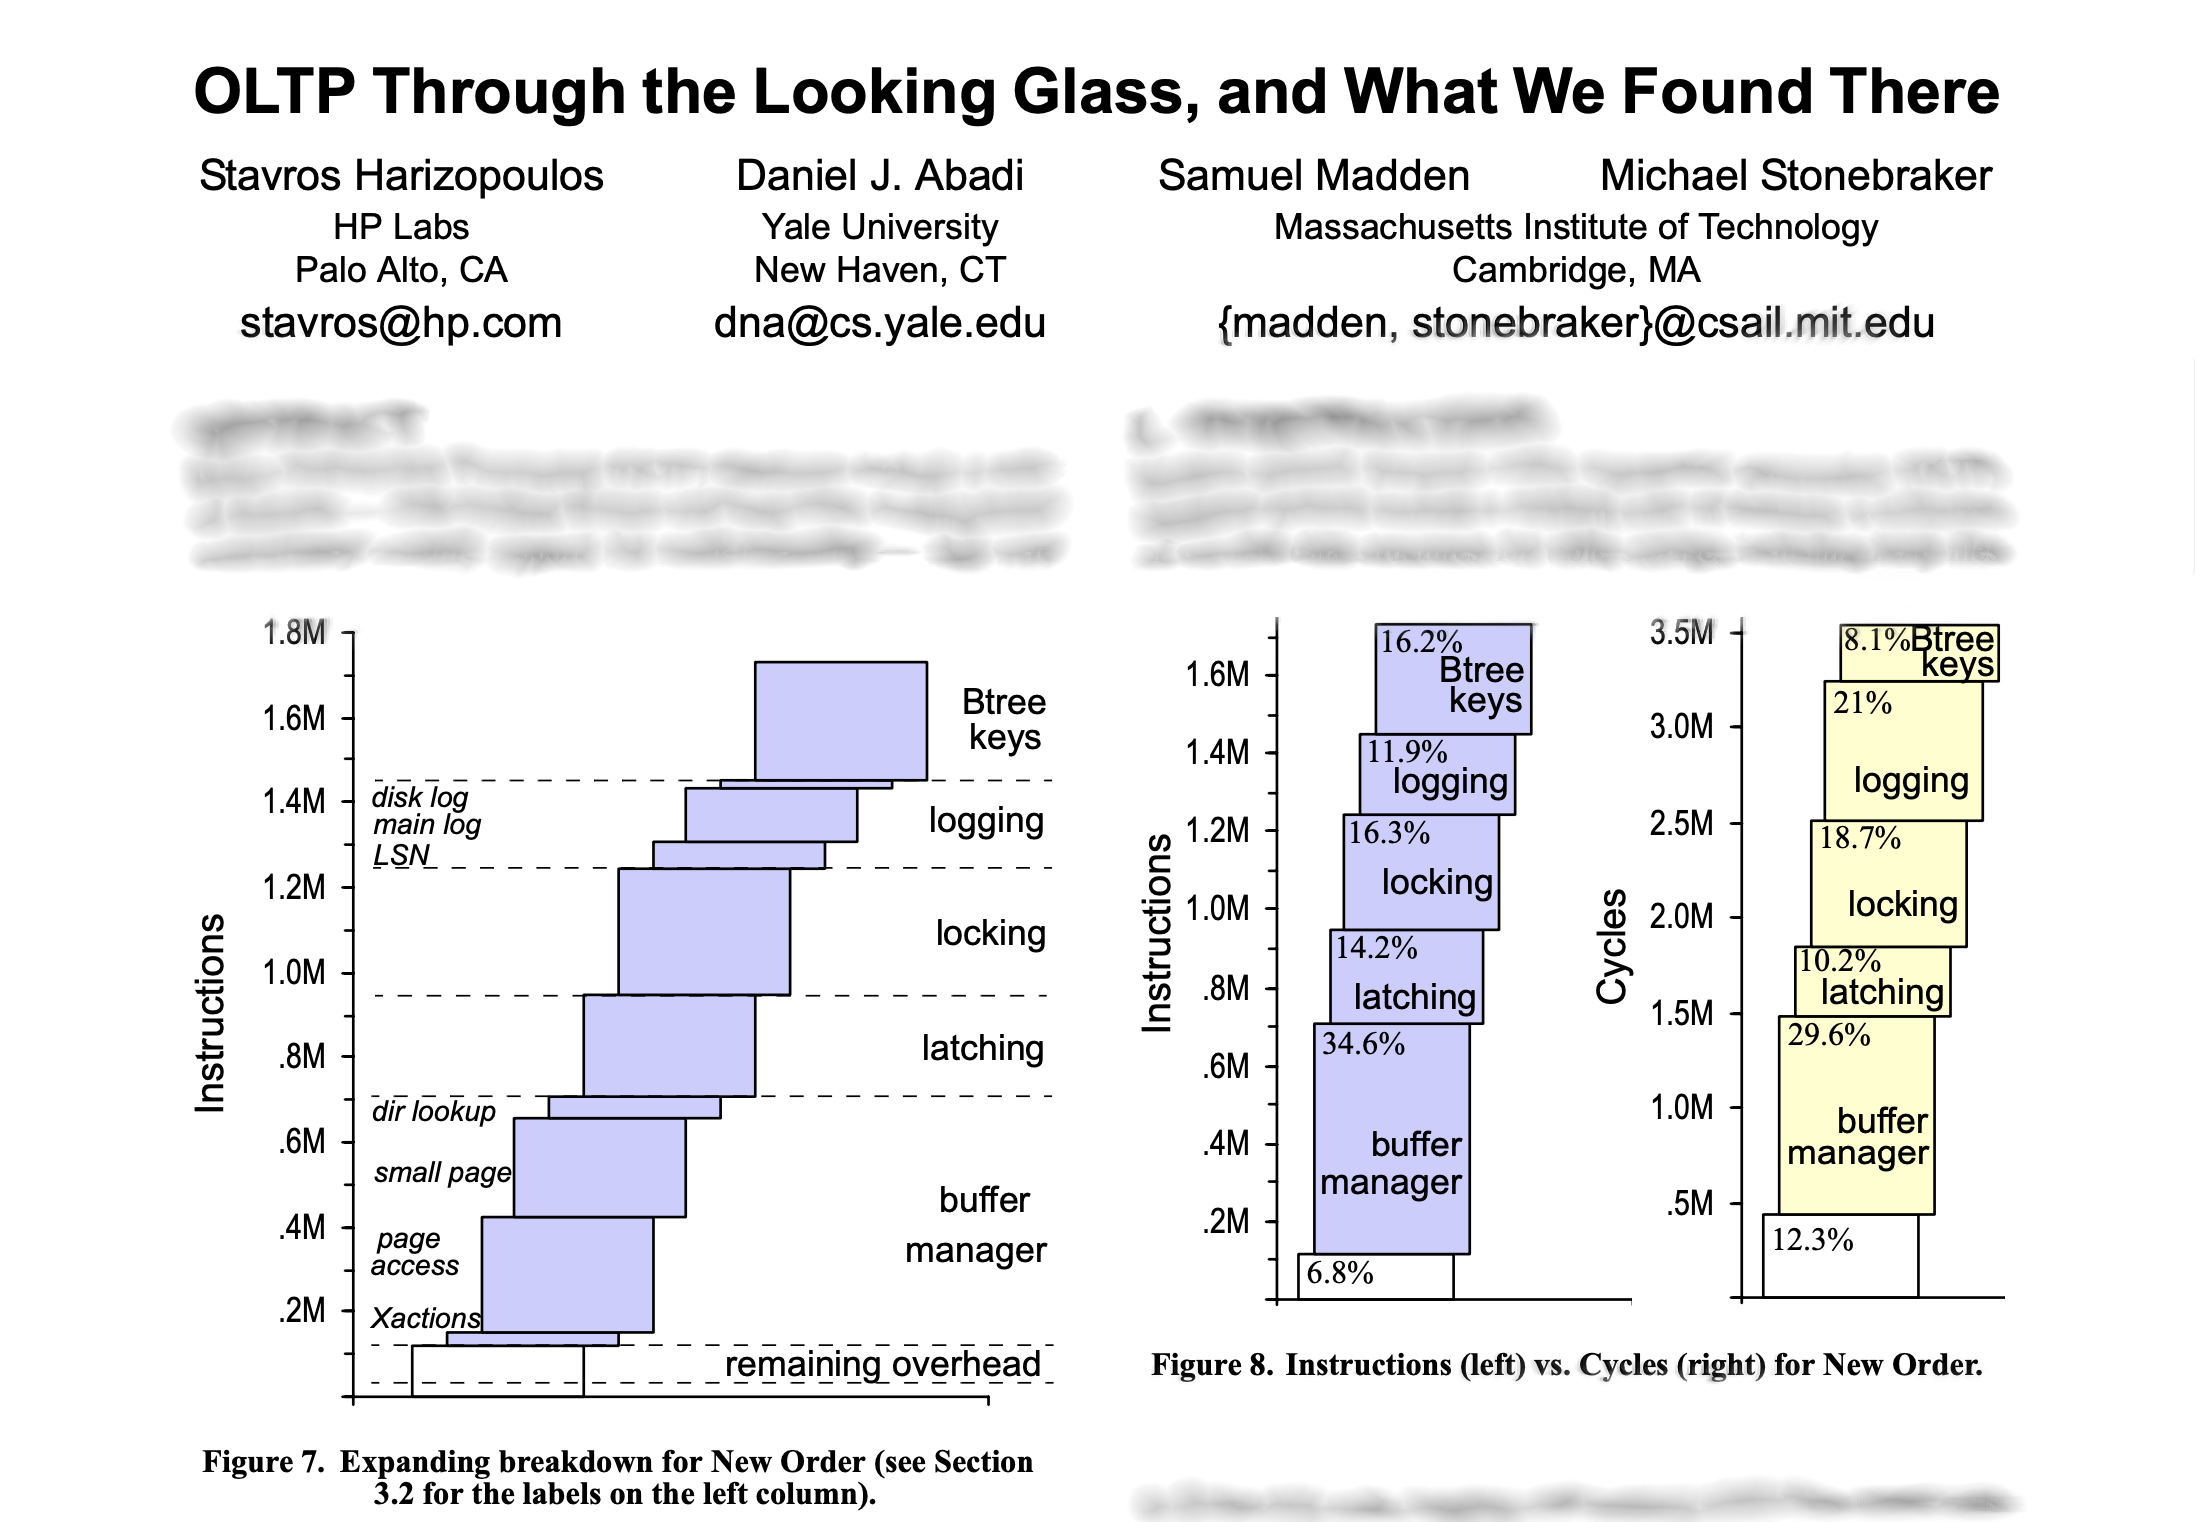
\includegraphics[width = \linewidth]{data/oltp_through_the_looking_glass.png}
\end{frame}

\begin{frame}
    \frametitle{The Author's Assumptions}

    \begin{itemize}
        \item<2->   No more larger-than-memory DBs
        \item<3->   Thus, multithreaded and interleaved transaction execution no more needed
        \item<4->   Many applications do not need ACID transactions
        \item<5->   Replication instead of logging for recovery
    \end{itemize}
\end{frame}

\begin{frame}
    \frametitle{The Author's Methodology}
    
    \uncover<2->{Gradually ...}
    \begin{itemize}
        \item<3->   ... make the DBS in-memory---removing buffer pool---, ...
        \item<4->   ... remove latching \uncover<5->{and locking, ...}
        \item<6->   ... remove transaction logging and LSN maintenance, ...
        \item<7->   ... and hand-optimize B-tree code for in-memory DBS.
    \end{itemize}
\end{frame}

\subsection{Results}

\frame{\subsectionpage}

\begin{frame}
    \frametitle{Read-Only YCSB}

    \pgfplotsset{%
        every axis/.append style = {
            ybar stacked,
            ylabel near ticks,
            y label style = {font = \small},
            ylabel shift = -.5em,
            ymode = normal,
            ymin = 0,
            ymax = 100,
            yticklabel style = {font = \scriptsize},
            ymode = normal,
            scaled y ticks = false,
            xmin = -0.25,
            xmax = 0.25,
            xtick = \empty,
            bar width = 0.5,
            ymajorgrids = false,
            width = .2875\textwidth,
            height = .85\paperheight
        }
    }

    \tikzset{%
        a0/.style = {black, fill = Cerulean},
        a1/.style = {black, fill = Cerulean!80},
        a2/.style = {black, fill = Cerulean!60},
        a3/.style = {black, fill = Cerulean!40},
        a4/.style = {black, fill = Cerulean!20},
        b0/.style = {black, fill = magenta},
        b1/.style = {black, fill = magenta!50},
        d/.style = {black, fill = white}
    }

    \Wider[6em]{%
        \centering
        \begin{tikzpicture}[remember picture,
                            visible on = <2->]
            \begin{axis}[ymax = 100]
                \node at ($(0, 0)!.5!(0, 8.27+0.13+4.44+4.14+5.30)$) {\makecell[c]{\contour{white}{Buffer pool}\\\footnotesize \contour{white}{\SI{22.28}{\percent}}}};
                \node at ($(0, 8.27+0.13+4.44+4.14+5.30)!.5!(0, 8.27+0.13+4.44+4.14+5.30+32.09+2.38)$) {\makecell[c]{\contour{white}{Locking}\\\footnotesize \contour{white}{\SI{34.47}{\percent}}}};
                \node at ($(0, 8.27+0.13+4.44+4.14+5.30+32.09+2.38)!.5!(0, 8.27+0.13+4.44+4.14+5.30+32.09+2.38+1.01)$) {\scriptsize\makecell[c]{\contour{white}{Logging \SI{1.01}{\percent}}}};
                \node at ($(0, 8.27+0.13+4.44+4.14+5.30+32.09+2.38+1.01)!.5!(0, 8.27+0.13+4.44+4.14+5.30+32.09+2.38+1.01+42.24)$) {\makecell[c]{\contour{white}{B-tree}\\\footnotesize \contour{white}{\SI{42.24}{\percent}}}};

                \addplot[d]                        coordinates       {(0, 0)};
                \addplot[a4]    coordinates       {(0, 8.27)};
                \addplot[a3]    coordinates       {(0, 0.13)};
                \addplot[a2]    coordinates       {(0, 4.44)};
                \addplot[a1]    coordinates       {(0, 4.14)};
                \addplot[a0]    coordinates       {(0, 5.30)};
                \addplot[b1]    coordinates       {(0, 32.09)};
                \addplot[b0]    coordinates       {(0, 2.38)};
                \addplot[a0]    coordinates       {(0, 1.01)};
                \addplot[b0]    coordinates       {(0, 42.24)};

                \coordinate (single0rest)            at (0.25, 0);
                \coordinate (single0bufferRest)      at (0.25, 8.27);
                \coordinate (single0bufferFreeList)  at (0.25, 8.27+0.13);
                \coordinate (single0bufferHashTable) at (0.25, 8.27+0.13+4.44);
                \coordinate (single0bufferFetching)  at (0.25, 8.27+0.13+4.44+4.14);
                \coordinate (single0bufferLatching)  at (0.25, 8.27+0.13+4.44+4.14+5.30);
                \coordinate (single0lockingRest)     at (0.25, 8.27+0.13+4.44+4.14+5.30+32.09);
                \coordinate (single0lockingLatching) at (0.25, 8.27+0.13+4.44+4.14+5.30+32.09+2.38);
            \end{axis}
        \end{tikzpicture}
        \hspace{.125em}
        \begin{tikzpicture}[remember picture,
                            visible on = <2->]
            \begin{axis}[ymax = 8.27+0.13+4.44+4.14+5.30+32.09+2.38]
                \node at ($(0, 8.27)!.5!(0, 8.27+0.13)$)  {\scriptsize\makecell[c]{\contour{white}{Free list \SI{0.13}{\percent}}}};
                \node at ($(0, 8.27+0.13)!.5!(0, 8.27+0.13+4.44)$) {\scriptsize\makecell[c]{\contour{white}{Hash table \SI{4.44}{\percent}}}};
                \node at ($(0, 8.27+0.13+4.44)!.5!(0, 8.27+0.13+4.44+4.14)$){\scriptsize\makecell[c]{\contour{white}{Fetching \SI{4.14}{\percent}}}};
                \node at ($(0, 8.27+0.13+4.44+4.14)!.5!(0, 8.27+0.13+4.44+4.14+5.30)$){\scriptsize\makecell[c]{\contour{white}{Latching \SI{5.3}{\percent}}}};
                \node[anchor = north, inner ysep = .5pt] at (0, 8.27+0.13+4.44+4.14+5.30+32.09+2.38){\scriptsize\makecell[c]{\contour{white}{Latching \SI{2.38}{\percent}}}};

                \addplot[a4] coordinates       {(0, 8.27)};
                \addplot[a3] coordinates       {(0, 0.13)};
                \addplot[a2] coordinates       {(0, 4.44)};
                \addplot[a1] coordinates       {(0, 4.14)};
                \addplot[a0] coordinates       {(0, 5.30)};
                \addplot[b1] coordinates       {(0, 32.09)};
                \addplot[b0] coordinates       {(0, 2.38)};

                \coordinate (single1rest)            at (-0.25, 0);
                \coordinate (single1bufferRest)      at (-0.25, 8.27);
                \coordinate (single1bufferFreeList)  at (-0.25, 8.27+0.13);
                \coordinate (single1bufferHashTable) at (-0.25, 8.27+0.13+4.44);
                \coordinate (single1bufferFetching)  at (-0.25, 8.27+0.13+4.44+4.14);
                \coordinate (single1bufferLatching)  at (-0.25, 8.27+0.13+4.44+4.14+5.30);
                \coordinate (single1lockingRest)     at (-0.25, 8.27+0.13+4.44+4.14+5.30+32.09);
                \coordinate (single1lockingLatching) at (-0.25, 8.27+0.13+4.44+4.14+5.30+32.09+2.38);
            \end{axis}
        \end{tikzpicture}
        \begin{tikzpicture}[remember picture,
                            overlay,
                            visible on = <2->]
            \draw (single0rest)[draw = black]            -- (single1rest);
            \draw (single0bufferRest)[draw = black]      -- (single1bufferRest);
            \draw (single0bufferFreeList)[draw = black]  -- (single1bufferFreeList);
            \draw (single0bufferHashTable)[draw = black] -- (single1bufferHashTable);
            \draw (single0bufferFetching)[draw = black]  -- (single1bufferFetching);
            \draw (single0bufferLatching)[draw = black]  -- (single1bufferLatching);
            \draw (single0lockingRest)[draw = black]     -- (single1lockingRest);
            \draw (single0lockingLatching)[draw = black] -- (single1lockingLatching);
        \end{tikzpicture}
        \hspace{-.5em}
        \begin{tikzpicture}[remember picture,
                            visible on = <3->]
            \begin{axis}[ymax = 100]
                \node at ($(0, 0)!.5!(0, 2.31+0.06+1.08+0.00+1.83)$) {\scriptsize\makecell[c]{\contour{white}{Buffer pool \SI{5.28}{\percent}}}};
                \node at ($(0, 2.31+0.06+1.08+0.00+1.83)!.5!(0, 2.31+0.06+1.08+0.00+1.83+27.65+49.94)$) {\makecell[c]{\contour{white}{Locking}\\\footnotesize \contour{white}{\SI{77.59}{\percent}}}};
                \node at ($(0, 2.31+0.06+1.08+0.00+1.83+27.65+49.94)!.5!(0, 2.31+0.06+1.08+0.00+1.83+27.65+49.94+0.36)$){\scriptsize\makecell[c]{\contour{white}{Logging \SI{0.36}{\percent}}}};
                \node at ($(0, 2.31+0.06+1.08+0.00+1.83+27.65+49.94+0.36)!.5!(0, 2.31+0.06+1.08+0.00+1.83+27.65+49.94+0.36+16.77)$){\makecell[c]{\contour{white}{B-tree}\\\footnotesize \contour{white}{\SI{16.77}{\percent}}}};

                \addplot[d]                         coordinates       {(0, 0)};
                \addplot[a4]     coordinates       {(0, 2.31)};
                \addplot[a3]     coordinates       {(0, 0.06)};
                \addplot[a2]     coordinates       {(0, 1.08)};
                \addplot[a0]     coordinates       {(0, 1.83)};
                \addplot[b1]    coordinates       {(0, 27.65)};
                \addplot[b0]    coordinates       {(0, 49.94)};
                \addplot[a0]    coordinates       {(0, 0.36)};
                \addplot[b0]    coordinates       {(0, 16.77)};

                \coordinate (multi0rest)            at (0.25, 0);
                \coordinate (multi0bufferRest)      at (0.25, 2.31);
                \coordinate (multi0bufferFreeList)  at (0.25, 2.31+0.06);
                \coordinate (multi0bufferHashTable) at (0.25, 2.31+0.06+1.08);
                \coordinate (multi0bufferFetching)  at (0.25, 2.31+0.06+1.08+0.00);
                \coordinate (multi0bufferLatching)  at (0.25, 2.31+0.06+1.08+0.00+1.83);
                \coordinate (multi0lockingRest)     at (0.25, 2.31+0.06+1.08+0.00+1.83+27.65);
                \coordinate (multi0lockingLatching) at (0.25, 2.31+0.06+1.08+0.00+1.83+27.65+49.94);
            \end{axis}
        \end{tikzpicture}
        \hspace{.125em}
        \begin{tikzpicture}[remember picture,
                            visible on = <3->]
            \begin{axis}[ymax = 2.31+0.06+1.08+0.00+1.83+27.65+49.94]
                \node at ($(0, 2.31)!.5!(0, 2.31+0.06)$){\scriptsize\makecell[c]{\contour{white}{Free list \SI{0.06}{\percent}}}};
                \node at ([yshift = .75em]$(0, 2.31)!.5!(0, 2.31+0.06)$) {\scriptsize\makecell[c]{\contour{white}{Hash table \SI{1.08}{\percent}}}};
                \node at ([yshift = 1.5em]$(0, 2.31)!.5!(0, 2.31+0.06)$){\scriptsize\makecell[c]{\contour{white}{Latching \SI{1.83}{\percent}}}};
                \node at ($(0, 2.31+0.06+1.08+0.00+1.83+27.65)!.5!(0, 2.31+0.06+1.08+0.00+1.83+27.65+49.94)$){\makecell[c]{\contour{white}{Latching}\\\footnotesize\contour{white}{\SI{49.94}{\percent}}}};

                \addplot[a4]    coordinates    {(0, 2.31)};
                \addplot[a3]    coordinates    {(0, 0.06)};
                \addplot[a2]    coordinates    {(0, 1.08)};
                \addplot[a0]    coordinates    {(0, 1.83)};
                \addplot[b1]    coordinates    {(0, 27.65)};
                \addplot[b0]    coordinates    {(0, 49.94)};

                \coordinate (multi1rest)            at (-0.25, 0);
                \coordinate (multi1bufferRest)      at (-0.25, 2.31);
                \coordinate (multi1bufferFreeList)  at (-0.25, 2.31+0.06);
                \coordinate (multi1bufferHashTable) at (-0.25, 2.31+0.06+1.08);
                \coordinate (multi1bufferFetching)  at (-0.25, 2.31+0.06+1.08+0.00);
                \coordinate (multi1bufferLatching)  at (-0.25, 2.31+0.06+1.08+0.00+1.83);
                \coordinate (multi1lockingRest)     at (-0.25, 2.31+0.06+1.08+0.00+1.83+27.65);
                \coordinate (multi1lockingLatching) at (-0.25, 2.31+0.06+1.08+0.00+1.83+27.65+49.94);
            \end{axis}
        \end{tikzpicture}
        \begin{tikzpicture}[remember picture,
                            overlay,
                            visible on = <3->]
            \draw (multi0rest)[draw = black]            -- (multi1rest);
            \draw (multi0bufferRest)[draw = black]      -- (multi1bufferRest);
            \draw (multi0bufferFreeList)[draw = black]  -- (multi1bufferFreeList);
            \draw (multi0bufferHashTable)[draw = black] -- (multi1bufferHashTable);
            \draw (multi0bufferFetching)[draw = black]  -- (multi1bufferFetching);
            \draw (multi0bufferLatching)[draw = black]  -- (multi1bufferLatching);
            \draw (multi0lockingRest)[draw = black]     -- (multi1lockingRest);
            \draw (multi0lockingLatching)[draw = black] -- (multi1lockingLatching);
        \end{tikzpicture}
    }
\end{frame}

\begin{frame}
    \frametitle{Update-Only YCSB}

    \pgfplotsset{%
        every axis/.append style = {
            ybar stacked,
            ylabel near ticks,
            y label style = {font = \small},
            ylabel shift = -.5em,
            ymode = normal,
            ymin = 0,
            ymax = 100,
            yticklabel style = {font = \scriptsize},
            ymode = normal,
            scaled y ticks = false,
            xmin = -0.25,
            xmax = 0.25,
            xtick = \empty,
            bar width = 0.5,
            ymajorgrids = false,
            width = .2875\textwidth,
            height = .85\paperheight
        }
    }
    
    \tikzset{%
        a0/.style = {black, fill = Cerulean},
        a1/.style = {black, fill = Cerulean!80},
        a2/.style = {black, fill = Cerulean!60},
        a3/.style = {black, fill = Cerulean!40},
        a4/.style = {black, fill = Cerulean!20},
        b0/.style = {black, fill = magenta},
        b1/.style = {black, fill = magenta!50},
        d/.style = {black, fill = white}
    }
    
    \Wider[6em]{%
        \centering
        \begin{tikzpicture}[remember picture,
                            visible on = <2->]
            \begin{axis}[ymax = 100]
                \node at ($(0, 0)!.5!(0, 6.17+0.07+3.46+1.17+5.17)$) {\makecell[c]{\contour{white}{Buffer pool}\\\footnotesize \contour{white}{\SI{16.04}{\percent}}}};
                \node at ($(0, 6.17+0.07+3.46+1.17+5.17)!.5!(0, 6.17+0.07+3.46+1.17+5.17+19.19+2.54)$) {\makecell[c]{\contour{white}{Locking}\\\footnotesize \contour{white}{\SI{21.73}{\percent}}}};
                \node at ($(0, 6.17+0.07+3.46+1.17+5.17+19.19+2.54)!.5!(0, 6.17+0.07+3.46+1.17+5.17+19.19+2.54+24.42)$) {\makecell[c]{\contour{white}{Logging}\\\footnotesize \contour{white}{\SI{24.42}{\percent}}}};
                \node at ($(0, 6.17+0.07+3.46+1.17+5.17+19.19+2.54+24.42)!.5!(0, 6.17+0.07+3.46+1.17+5.17+19.19+2.54+24.42+37.81)$) {\makecell[c]{\contour{white}{B-tree}\\\footnotesize \contour{white}{\SI{37.81}{\percent}}}};
                
                \addplot[d]                     coordinates       {(0, 0)};
                \addplot[a4] coordinates       {(0, 6.17)};
                \addplot[a3] coordinates       {(0, 0.07)};
                \addplot[a2] coordinates       {(0, 3.46)};
                \addplot[a1] coordinates       {(0, 1.17)};
                \addplot[a0] coordinates       {(0, 5.17)};
                \addplot[b1] coordinates       {(0, 19.19)};
                \addplot[b0] coordinates       {(0, 2.54)};
                \addplot[a0] coordinates       {(0, 24.42)};
                \addplot[b0] coordinates       {(0, 37.81)};
                
                \coordinate (single0rest)            at (0.25, 0);
                \coordinate (single0bufferRest)      at (0.25, 6.17);
                \coordinate (single0bufferFreeList)  at (0.25, 6.17+0.07);
                \coordinate (single0bufferHashTable) at (0.25, 6.17+0.07+3.46);
                \coordinate (single0bufferFetching)  at (0.25, 6.17+0.07+3.46+1.17);
                \coordinate (single0bufferLatching)  at (0.25, 6.17+0.07+3.46+1.17+5.17);
                \coordinate (single0lockingRest)     at (0.25, 6.17+0.07+3.46+1.17+5.17+19.19);
                \coordinate (single0lockingLatching) at (0.25, 6.17+0.07+3.46+1.17+5.17+19.19+2.54);
            \end{axis}
        \end{tikzpicture}
        \hspace{.125em}
        \begin{tikzpicture}[remember picture,
                            visible on = <2->]
            \begin{axis}[ymax = 6.17+0.07+3.46+1.17+5.17+19.19+2.54]
                \node at ($(0, 6.17)!.5!(0, 6.17+0.07)$)  {\scriptsize\makecell[c]{\contour{white}{Free list \SI{0.07}{\percent}}}};
                \node at ($(0, 6.17+0.07)!.5!(0, 6.17+0.07+3.46)$) {\scriptsize\makecell[c]{\contour{white}{Hash table \SI{3.46}{\percent}}}};
                \node at ($(0, 6.17+0.07+3.46)!.5!(0, 6.17+0.07+3.46+1.17)$){\scriptsize\makecell[c]{\contour{white}{Fetching \SI{1.17}{\percent}}}};
                \node at ($(0, 6.17+0.07+3.46+1.17)!.5!(0, 6.17+0.07+3.46+1.17+5.17)$){\scriptsize\makecell[c]{\contour{white}{Latching \SI{5.17}{\percent}}}};
                \node at ($(0, 6.17+0.07+3.46+1.17+5.17+19.19)!.5!(0, 6.17+0.07+3.46+1.17+5.17+19.19+2.54)$){\scriptsize\makecell[c]{\contour{white}{Latching \SI{2.54}{\percent}}}};
                
                \addplot[a4] coordinates       {(0, 6.17)};
                \addplot[a3] coordinates       {(0, 0.07)};
                \addplot[a2] coordinates       {(0, 3.46)};
                \addplot[a1] coordinates       {(0, 1.17)};
                \addplot[a0] coordinates       {(0, 5.17)};
                \addplot[b1] coordinates       {(0, 19.19)};
                \addplot[b0] coordinates       {(0, 2.54)};
                
                \coordinate (single1rest)            at (-0.25, 0);
                \coordinate (single1bufferRest)      at (-0.25, 6.17);
                \coordinate (single1bufferFreeList)  at (-0.25, 6.17+0.07);
                \coordinate (single1bufferHashTable) at (-0.25, 6.17+0.07+3.46);
                \coordinate (single1bufferFetching)  at (-0.25, 6.17+0.07+3.46+1.17);
                \coordinate (single1bufferLatching)  at (-0.25, 6.17+0.07+3.46+1.17+5.17);
                \coordinate (single1lockingRest)     at (-0.25, 6.17+0.07+3.46+1.17+5.17+19.19);
                \coordinate (single1lockingLatching) at (-0.25, 6.17+0.07+3.46+1.17+5.17+19.19+2.54);
            \end{axis}
        \end{tikzpicture}
        \begin{tikzpicture}[remember picture,
                            overlay,
                            visible on = <2->]
            \draw (single0rest)[draw = black]            -- (single1rest);
            \draw (single0bufferRest)[draw = black]      -- (single1bufferRest);
            \draw (single0bufferFreeList)[draw = black]  -- (single1bufferFreeList);
            \draw (single0bufferHashTable)[draw = black] -- (single1bufferHashTable);
            \draw (single0bufferFetching)[draw = black]  -- (single1bufferFetching);
            \draw (single0bufferLatching)[draw = black]  -- (single1bufferLatching);
            \draw (single0lockingRest)[draw = black]     -- (single1lockingRest);
            \draw (single0lockingLatching)[draw = black] -- (single1lockingLatching);
        \end{tikzpicture}
        \hspace{-.5em}
        \begin{tikzpicture}[remember picture,
                            visible on = <3->]
            \begin{axis}[ymax = 100]
                \node at ($(0, 0)!.5!(0, 2.35+0.05+1.12+0.03+2.44)$) {\scriptsize\makecell[c]{\contour{white}{Buffer pool \SI{5.99}{\percent}}}};
                \node at ($(0, 2.35+0.05+1.12+0.03+2.44)!.5!(0, 2.35+0.05+1.12+0.03+2.44+10.28+40.28)$) {\makecell[c]{\contour{white}{Locking}\\\footnotesize \contour{white}{\SI{50.55}{\percent}}}};
                \node at ($(0, 2.35+0.05+1.12+0.03+2.44+10.28+40.28)!.5!(0, 2.35+0.05+1.12+0.03+2.44+10.28+40.28+27.85)$) {\makecell[c]{\contour{white}{Logging}\\\footnotesize \contour{white}{\SI{27.85}{\percent}}}};
                \node at ($(0, 2.35+0.05+1.12+0.03+2.44+10.28+40.28+27.85)!.5!(0, 2.35+0.05+1.12+0.03+2.44+10.28+40.28+27.85+15.60)$) {\makecell[c]{\contour{white}{B-tree}\\\footnotesize \contour{white}{\SI{15.6}{\percent}}}};
                
                \addplot[d]                         coordinates       {(0, 0)};
                \addplot[a4]     coordinates       {(0, 2.35)};
                \addplot[a3]     coordinates       {(0, 0.05)};
                \addplot[a2]     coordinates       {(0, 1.12)};
                \addplot[a1]     coordinates       {(0, 0.03)};
                \addplot[a0]     coordinates       {(0, 2.44)};
                \addplot[b1]    coordinates       {(0, 10.28)};
                \addplot[b0]    coordinates       {(0, 40.28)};
                \addplot[a0]    coordinates       {(0, 27.85)};
                \addplot[b0]    coordinates       {(0, 15.60)};
                
                \coordinate (multi0rest)            at (0.25, 0);
                \coordinate (multi0bufferRest)      at (0.25, 2.35);
                \coordinate (multi0bufferFreeList)  at (0.25, 2.35+0.05);
                \coordinate (multi0bufferHashTable) at (0.25, 2.35+0.05+1.12);
                \coordinate (multi0bufferFetching)  at (0.25, 2.35+0.05+1.12+0.03);
                \coordinate (multi0bufferLatching)  at (0.25, 2.35+0.05+1.12+0.03+2.44);
                \coordinate (multi0lockingRest)     at (0.25, 2.35+0.05+1.12+0.03+2.44+10.28);
                \coordinate (multi0lockingLatching) at (0.25, 2.35+0.05+1.12+0.03+2.44+10.28+40.28);
            \end{axis}
        \end{tikzpicture}
        \hspace{.125em}
        \begin{tikzpicture}[remember picture,
                            visible on = <3->]
            \begin{axis}[ymax = 2.35+0.05+1.12+0.03+2.44+10.28+40.28]
                \node at ($(0, 2.35)!.5!(0, 2.35+0.05)$)  {\scriptsize\makecell[c]{\contour{white}{Free list \SI{0.05}{\percent}}}};
                \node at ([yshift = .75em]$(0, 2.35)!.5!(0, 2.35+0.05)$) {\scriptsize\makecell[c]{\contour{white}{Hash table \SI{1.12}{\percent}}}};
                \node at ([yshift = 1.5em]$(0, 2.35)!.5!(0, 2.35+0.05)$){\scriptsize\makecell[c]{\contour{white}{Fetching \SI{0.03}{\percent}}}};
                \node at ([yshift = 2.25em]$(0, 2.35)!.5!(0, 2.35+0.05)$){\scriptsize\makecell[c]{\contour{white}{Latching \SI{2.44}{\percent}}}};
                \node at ($(0, 2.35+0.05+1.12+0.03+2.44+10.28)!.5!(0, 2.35+0.05+1.12+0.03+2.44+10.28+40.28)$){\scriptsize\makecell[c]{\contour{white}{Latching \SI{40.28}{\percent}}}};
                
                \addplot[a4]    coordinates       {(0, 2.35)};
                \addplot[a3]    coordinates       {(0, 0.05)};
                \addplot[a2]    coordinates       {(0, 1.12)};
                \addplot[a1]    coordinates       {(0, 0.03)};
                \addplot[a0]    coordinates       {(0, 2.44)};
                \addplot[b1]    coordinates       {(0, 10.28)};
                \addplot[b0]    coordinates       {(0, 40.28)};
                
                \coordinate (multi1rest)            at (-0.25, 0);
                \coordinate (multi1bufferRest)      at (-0.25, 2.35);
                \coordinate (multi1bufferFreeList)  at (-0.25, 2.35+0.05);
                \coordinate (multi1bufferHashTable) at (-0.25, 2.35+0.05+1.12);
                \coordinate (multi1bufferFetching)  at (-0.25, 2.35+0.05+1.12+0.03);
                \coordinate (multi1bufferLatching)  at (-0.25, 2.35+0.05+1.12+0.03+2.44);
                \coordinate (multi1lockingRest)     at (-0.25, 2.35+0.05+1.12+0.03+2.44+10.28);
                \coordinate (multi1lockingLatching) at (-0.25, 2.35+0.05+1.12+0.03+2.44+10.28+40.28);
            \end{axis}
        \end{tikzpicture}
        \begin{tikzpicture}[remember picture,
                            overlay,
                            visible on = <3->]
            \draw (multi0rest)[draw = black]            -- (multi1rest);
            \draw (multi0bufferRest)[draw = black]      -- (multi1bufferRest);
            \draw (multi0bufferFreeList)[draw = black]  -- (multi1bufferFreeList);
            \draw (multi0bufferHashTable)[draw = black] -- (multi1bufferHashTable);
            \draw (multi0bufferFetching)[draw = black]  -- (multi1bufferFetching);
            \draw (multi0bufferLatching)[draw = black]  -- (multi1bufferLatching);
            \draw (multi0lockingRest)[draw = black]     -- (multi1lockingRest);
            \draw (multi0lockingLatching)[draw = black] -- (multi1lockingLatching);
        \end{tikzpicture}
    }
\end{frame}

\begin{frame}
    \frametitle{TPC-C}
    
    \pgfplotsset{%
        every axis/.append style = {
            ybar stacked,
            ylabel near ticks,
            y label style = {font = \small},
            ylabel shift = -.5em,
            ymode = normal,
            ymin = 0,
            ymax = 100,
            yticklabel style = {font = \scriptsize},
            ymode = normal,
            scaled y ticks = false,
            xmin = -0.25,
            xmax = 0.25,
            xtick = \empty,
            bar width = 0.5,
            ymajorgrids = false,
            width = .2875\textwidth,
            height = .85\paperheight
        }
    }
    
    \tikzset{%
        a0/.style = {black, fill = Cerulean},
        a1/.style = {black, fill = Cerulean!80},
        a2/.style = {black, fill = Cerulean!60},
        a3/.style = {black, fill = Cerulean!40},
        a4/.style = {black, fill = Cerulean!20},
        b0/.style = {black, fill = magenta},
        b1/.style = {black, fill = magenta!50},
        d/.style = {black, fill = white}
    }
    
    \Wider[6em]{%
        \centering
        \begin{tikzpicture}[remember picture,
                            visible on = <2->]
            \begin{axis}[ymax = 100]
                \node at ($(0, 0)!.5!(0, 8.84+0.05+4.56+0.49+6.17)$) {\makecell[c]{\contour{white}{Buffer pool}\\\footnotesize \contour{white}{\SI{20.11}{\percent}}}};
                \node at ($(0, 8.84+0.05+4.56+0.49+6.17)!.5!(0, 8.84+0.05+4.56+0.49+6.17+4.55+0.36)$) {\scriptsize\makecell[c]{\contour{white}{Locking \SI{4.91}{\percent}}}};
                \node at ($(0, 8.84+0.05+4.56+0.49+6.17+4.55+0.36)!.5!(0, 8.84+0.05+4.56+0.49+6.17+4.55+0.36+42.46)$) {\makecell[c]{\contour{white}{Logging}\\\footnotesize \contour{white}{\SI{42.46}{\percent}}}};
                \node at ($(0, 8.84+0.05+4.56+0.49+6.17+4.55+0.36+42.46)!.5!(0, 8.84+0.05+4.56+0.49+6.17+4.55+0.36+42.46+32.51)$) {\makecell[c]{\contour{white}{B-tree}\\\footnotesize \contour{white}{\SI{32.51}{\percent}}}};
                
                \addplot[d]                     coordinates       {(0, 0)};
                \addplot[a4] coordinates       {(0, 8.84)};
                \addplot[a3] coordinates       {(0, 0.05)};
                \addplot[a2] coordinates       {(0, 4.56)};
                \addplot[a1] coordinates       {(0, 0.49)};
                \addplot[a0] coordinates       {(0, 6.17)};
                \addplot[b1] coordinates       {(0, 4.55)};
                \addplot[b0] coordinates       {(0, 0.36)};
                \addplot[a0] coordinates       {(0, 42.46)};
                \addplot[b0] coordinates       {(0, 32.51)};
                
                \coordinate (single0rest)            at (0.25, 0);
                \coordinate (single0bufferRest)      at (0.25, 8.84);
                \coordinate (single0bufferFreeList)  at (0.25, 8.84+0.05);
                \coordinate (single0bufferHashTable) at (0.25, 8.84+0.05+4.56);
                \coordinate (single0bufferFetching)  at (0.25, 8.84+0.05+4.56+0.49);
                \coordinate (single0bufferLatching)  at (0.25, 8.84+0.05+4.56+0.49+6.17);
                \coordinate (single0lockingRest)     at (0.25, 8.84+0.05+4.56+0.49+6.17+4.55);
                \coordinate (single0lockingLatching) at (0.25, 8.84+0.05+4.56+0.49+6.17+4.55+0.36);
            \end{axis}
        \end{tikzpicture}
        \hspace{.125em}
        \begin{tikzpicture}[remember picture,
                            visible on = <2->]
            \begin{axis}[ymax = 8.84+0.05+4.56+0.49+6.17+4.55+0.36]
                \node at ($(0, 8.84)!.5!(0, 8.84+0.05)$)  {\scriptsize\makecell[c]{\contour{white}{Free list \SI{0.05}{\percent}}}};
                \node at ($(0, 8.84+0.05)!.5!(0, 8.84+0.05+4.56)$) {\makecell[c]{\contour{white}{Hash table}\\\footnotesize \contour{white}{\SI{4.56}{\percent}}}};
                \node at ($(0, 8.84+0.05+4.56)!.5!(0, 8.84+0.05+4.56+0.49)$){\scriptsize\makecell[c]{\contour{white}{Fetching} \contour{white}{\SI{0.49}{\percent}}}};
                \node at ($(0, 8.84+0.05+4.56+0.49)!.5!(0, 8.84+0.05+4.56+0.49+6.17)$){\makecell[c]{\contour{white}{Latching}\\\footnotesize \contour{white}{\SI{6.17}{\percent}}}};
                \node[anchor = north, inner ysep = .5pt] at (0, 8.84+0.05+4.56+0.49+6.17+4.55+0.36){\scriptsize\makecell[c]{\contour{white}{Latching \SI{0.36}{\percent}}}};
                
                \addplot[a4] coordinates       {(0, 8.84)};
                \addplot[a3] coordinates       {(0, 0.05)};
                \addplot[a2] coordinates       {(0, 4.56)};
                \addplot[a1] coordinates       {(0, 0.49)};
                \addplot[a0] coordinates       {(0, 6.17)};
                \addplot[b1] coordinates       {(0, 4.55)};
                \addplot[b0] coordinates       {(0, 0.36)};
                
                \coordinate (single1rest)            at (-0.25, 0);
                \coordinate (single1bufferRest)      at (-0.25, 8.84);
                \coordinate (single1bufferFreeList)  at (-0.25, 8.84+0.05);
                \coordinate (single1bufferHashTable) at (-0.25, 8.84+0.05+4.56);
                \coordinate (single1bufferFetching)  at (-0.25, 8.84+0.05+4.56+0.49);
                \coordinate (single1bufferLatching)  at (-0.25, 8.84+0.05+4.56+0.49+6.17);
                \coordinate (single1lockingRest)     at (-0.25, 8.84+0.05+4.56+0.49+6.17+4.55);
                \coordinate (single1lockingLatching) at (-0.25, 8.84+0.05+4.56+0.49+6.17+4.55+0.36);
            \end{axis}
        \end{tikzpicture}
        \begin{tikzpicture}[remember picture,
                            overlay,
                            visible on = <2->]
            \draw (single0rest)[draw = black]            -- (single1rest);
            \draw (single0bufferRest)[draw = black]      -- (single1bufferRest);
            \draw (single0bufferFreeList)[draw = black]  -- (single1bufferFreeList);
            \draw (single0bufferHashTable)[draw = black] -- (single1bufferHashTable);
            \draw (single0bufferFetching)[draw = black]  -- (single1bufferFetching);
            \draw (single0bufferLatching)[draw = black]  -- (single1bufferLatching);
            \draw (single0lockingRest)[draw = black]     -- (single1lockingRest);
            \draw (single0lockingLatching)[draw = black] -- (single1lockingLatching);
        \end{tikzpicture}
        \hspace{-.5em}
        \begin{tikzpicture}[remember picture,
                            visible on = <3->]
            \begin{axis}[ymax = 100]
                \node at ($(0, 0)!.5!(0, 8.61+0.22+4.01+0.05+8.99)$) {\makecell[c]{\contour{white}{Buffer pool}\\\footnotesize \contour{white}{\SI{21.87}{\percent}}}};
                \node at ($(0, 8.61+0.22+4.01+0.05+8.99)!.5!(0, 8.61+0.22+4.01+0.05+8.99+3.79+0.76)$) {\scriptsize\makecell[c]{\contour{white}{Locking \SI{4.55}{\percent}}}};
                \node at ($(0, 8.61+0.22+4.01+0.05+8.99+3.79+0.76)!.5!(0, 8.61+0.22+4.01+0.05+8.99+3.79+0.76+8.45)$) {\makecell[c]{\scriptsize\contour{white}{Logging \SI{8.45}{\percent}}}};
                \node at ($(0, 8.61+0.22+4.01+0.05+8.99+3.79+0.76+8.45)!.5!(0, 8.61+0.22+4.01+0.05+8.99+3.79+0.76+8.45+65.12)$) {\makecell[c]{\contour{white}{B-tree}\\\footnotesize \contour{white}{\SI{65.12}{\percent}}}};
                
                \addplot[d]                         coordinates       {(0, 0)};
                \addplot[a4]     coordinates       {(0, 8.61)};
                \addplot[a3]     coordinates       {(0, 0.22)};
                \addplot[a2]     coordinates       {(0, 4.01)};
                \addplot[a1]     coordinates       {(0, 0.05)};
                \addplot[a0]     coordinates       {(0, 8.99)};
                \addplot[b1]    coordinates       {(0, 3.79)};
                \addplot[b0]    coordinates       {(0, 0.76)};
                \addplot[a0]    coordinates       {(0, 8.45)};
                \addplot[b0]    coordinates       {(0, 65.12)};
                
                \coordinate (multi0rest)            at (0.25, 0);
                \coordinate (multi0bufferRest)      at (0.25, 8.61);
                \coordinate (multi0bufferFreeList)  at (0.25, 8.61+0.22);
                \coordinate (multi0bufferHashTable) at (0.25, 8.61+0.22+4.01);
                \coordinate (multi0bufferFetching)  at (0.25, 8.61+0.22+4.01+0.05);
                \coordinate (multi0bufferLatching)  at (0.25, 8.61+0.22+4.01+0.05+8.99);
                \coordinate (multi0lockingRest)     at (0.25, 8.61+0.22+4.01+0.05+8.99+3.79);
                \coordinate (multi0lockingLatching) at (0.25, 8.61+0.22+4.01+0.05+8.99+3.79+0.76);
            \end{axis}
        \end{tikzpicture}
        \hspace{.125em}
        \begin{tikzpicture}[remember picture,
                            visible on = <3->]
            \begin{axis}[ymax = 8.61+0.22+4.01+0.05+8.99+3.79+0.76]
                \node at ($(0, 8.61)!.5!(0, 8.61+0.22)$)  {\scriptsize\makecell[c]{\contour{white}{Free list \SI{0.22}{\percent}}}};
                \node at ($(0, 8.61+0.22)!.5!(0, 8.61+0.22+4.01)$) {\makecell[c]{\contour{white}{Hash table}\\\footnotesize \contour{white}{\SI{4.01}{\percent}}}};
                \node at ($(0, 8.61+0.22+4.01)!.5!(0, 8.61+0.22+4.01+0.05)$){\scriptsize\makecell[c]{\contour{white}{Fetching} \contour{white}{\SI{0.05}{\percent}}}};
                \node at ($(0, 8.61+0.22+4.01+0.05)!.5!(0, 8.61+0.22+4.01+0.05+8.99)$){\makecell[c]{\contour{white}{Latching}\\\footnotesize \contour{white}{\SI{8.99}{\percent}}}};
                \node[anchor = north, inner ysep = .5pt] at (0, 8.61+0.22+4.01+0.05+8.99+3.79+0.76){\scriptsize\makecell[c]{\contour{white}{Latching \SI{0.76}{\percent}}}};
                
                \addplot[a4]    coordinates       {(0, 8.61)};
                \addplot[a3]    coordinates       {(0, 0.22)};
                \addplot[a2]    coordinates       {(0, 4.01)};
                \addplot[a1]    coordinates       {(0, 0.05)};
                \addplot[a0]    coordinates       {(0, 8.99)};
                \addplot[b1]    coordinates       {(0, 3.79)};
                \addplot[b0]    coordinates       {(0, 0.76)};
                
                \coordinate (multi1rest)            at (-0.25, 0);
                \coordinate (multi1bufferRest)      at (-0.25, 8.61);
                \coordinate (multi1bufferFreeList)  at (-0.25, 8.61+0.22);
                \coordinate (multi1bufferHashTable) at (-0.25, 8.61+0.22+4.01);
                \coordinate (multi1bufferFetching)  at (-0.25, 8.61+0.22+4.01+0.05);
                \coordinate (multi1bufferLatching)  at (-0.25, 8.61+0.22+4.01+0.05+8.99);
                \coordinate (multi1lockingRest)     at (-0.25, 8.61+0.22+4.01+0.05+8.99+3.79);
                \coordinate (multi1lockingLatching) at (-0.25, 8.61+0.22+4.01+0.05+8.99+3.79+0.76);
            \end{axis}
        \end{tikzpicture}
        \begin{tikzpicture}[remember picture,
                            overlay,
                            visible on = <3->]
            \draw (multi0rest)[draw = black]            -- (multi1rest);
            \draw (multi0bufferRest)[draw = black]      -- (multi1bufferRest);
            \draw (multi0bufferFreeList)[draw = black]  -- (multi1bufferFreeList);
            \draw (multi0bufferHashTable)[draw = black] -- (multi1bufferHashTable);
            \draw (multi0bufferFetching)[draw = black]  -- (multi1bufferFetching);
            \draw (multi0bufferLatching)[draw = black]  -- (multi1bufferLatching);
            \draw (multi0lockingRest)[draw = black]     -- (multi1lockingRest);
            \draw (multi0lockingLatching)[draw = black] -- (multi1lockingLatching);
        \end{tikzpicture}
    }
\end{frame}

\subsection{Conclusion}

\begin{frame}
    \frametitle{\insertsubsection}

    \begin{block}<2->{Complex OLTP (and OLAP)}
        The index structures (here Foster B-tree) are the most performance-critical components.
    \end{block}
    \begin{block}<3->{Simple Workloads}
        A global latch in the transaction manager limits the performance.
\end{block}
\end{frame}

\subsection{Optimizations of OLTP Systems}

\frame{\subsectionpage}

\begin{frame}
    \frametitle[Buffer Pool Pointer Swizzling]{Pointer Swizzling in the Buffer Pool \cite{Graefe:2014}}

    \pgfplotsset{%
        every axis/.append style = {
            yticklabel style = {font = \scriptsize},
            scaled y ticks = false,
            ybar = .8pt,
            bar width = .5em,
            xmin = -0.5,
            xmax = 14.5,
            xtick style = {draw = none},
            xtick = {0, 1, 2, 3, 4, 5, 6, 7, 8, 9, 10, 11, 12, 13, 14},
            xticklabels = {{\SI{100}{\mega\byte}}, {\SI{200}{\mega\byte}}, {\SI{400}{\mega\byte}}, {\SI{600}{\mega\byte}}, {\SI{800}{\mega\byte}}, {\SI{1}{\giga\byte}}, {\SI{2}{\giga\byte}}, {\SI{4}{\giga\byte}}, {\SI{6}{\giga\byte}}, {\SI{8}{\giga\byte}}, {\SI{10}{\giga\byte}}, {\SI{15}{\giga\byte}}, {\SI{20}{\giga\byte}}, {\SI{25}{\giga\byte}}, {\SI{30}{\giga\byte}}},
            x tick label style = {align = center,
                                  font = \footnotesize,
                                  rotate = 45,
                                  yshift = 1em},
            xlabel near ticks,
            x label style = {font = \small},
            legend style = {font = \tiny,
                            legend columns = -1,
                            /tikz/every even column/.append style = {column sep = 0.05cm},
                            row sep = -2pt,
                            draw = none,
                            fill = none,
                            at = {(0.5, 0.97)},
                            anchor = north},
            width = .925\textwidth,
            height = .8\paperheight
        }
    }
    
    \tikzset{%
        noSwizzling/.style = {thick, draw = Cerulean, fill = Cerulean!50},
        swizzling/.style = {thick, draw = Magenta, fill = Magenta!50}
    }

    \centering
    \begin{tikzpicture}
        \begin{axis}[ymode = normal,
                     ymin = 0,
                     ymajorgrids = true,
                     yticklabel style = {/pgf/number format/fixed}]
            \addplot[noSwizzling] coordinates
                {(0, 66369.56) (1, 74553.61) (2, 81580.19) (3, 84328.74) (4, 93443.81) (5, 96880.01) (6, 125655.94) (7, 193685.35) (8, 345966.01) (9, 575737.3) (10, 745879.28) (11, 817851.23) (12, 825045.18) (13, 845368.47) (14, 883277.13)};
            \addlegendentry{Without pointer swizzling};
            \addplot[swizzling, visible on = <2->] coordinates
                {(0, 63542.98) (1, 73687.28) (2, 83746.49) (3, 83687.17) (4, 90374.45) (5, 94442.6) (6, 123271.54) (7, 189535.78) (8, 334771.48) (9, 539832.4) (10, 676508.03) (11, 799808.39) (12, 815658.29) (13, 844863.03) (14, 887174.57)};
            \addlegendentry[visible on = <2->]{With pointer swizzling};
        \end{axis}
    \end{tikzpicture}
\end{frame}

\begin{frame}
    \frametitle{System Call: bzero}

    \centering
    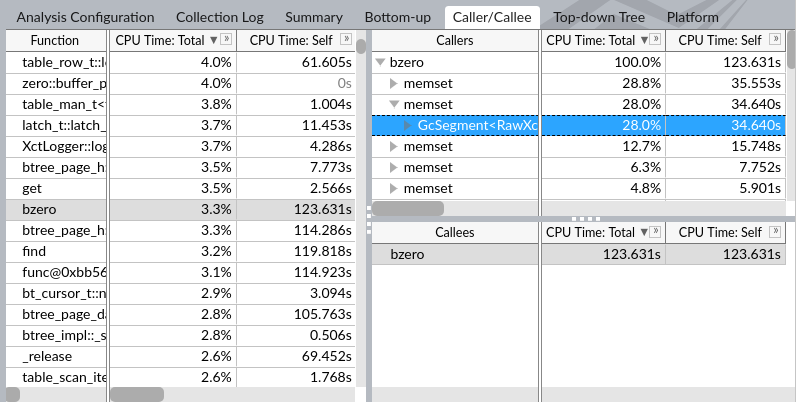
\includegraphics[width = \linewidth]{data/bzero.png}\\
\end{frame}

\begin{frame}
    \frametitle{System Call: bzero}

    \pgfplotsset{%
        every axis/.append style = {
            xlabel = {$\text{Transaction throughput }\left[\si{1\per\minute}\right]$},
            xlabel near ticks,
            x label style = {font = \small},
            xticklabel style = {font = \scriptsize,
                                /pgf/number format/fixed,
                                rotate = 30,
                                align = center},
            xmode = normal,
            xmin = 0,
            scaled x ticks = false,
            xbar = .8pt,
            ymin = -0.75,
            ymax = 1.75,
            bar width = 2.5em,
            ytick style = {draw = none},
            ytick = {0, 1},
            yticklabels = {Optimized, Baseline},
            y tick label style = {align = center,
                                  font = \footnotesize},
            ylabel near ticks,
            y label style = {font = \small},
            xmajorgrids = true,
            width = \textwidth,
            height = .5\paperheight
        }
    }
    \begin{tikzpicture}
        \begin{axis}
            \addplot[draw = Cerulean, fill = Cerulean!50] coordinates
                {(889279.6, 0) (883277.13, 1)};
        \end{axis}
    \end{tikzpicture}
\end{frame}

%------------------------------------------------
%\section*{References}
%------------------------------------------------

\begin{frame}[noframenumbering, allowframebreaks]{References}
    \printbibliography
\end{frame}

%------------------------------------------------
\section*{End}
%------------------------------------------------

\begin{frame}
\Huge{\centerline{Your Turn to Ask ...}}
\end{frame}

    \addtocontents{toc}{\protect\setcounter{tocdepth}{0}}

%\section[]{Appendix}

\begin{frame}
    \frametitle[Classification by Bélády]{Page Replacement Algorithm Classification by Bélády From \cite{Belady:1966}}
    
    \begin{description}
        \item<2-7>[Class 1]    \alt<2-2>{No statistics}{RANDOM, FIFO and FILO}
        \item<4-7>[Class 2]    \alt<4-4>{Statistics about the latest references of \emph{pages in the buffer pool\vspace{\baselineskip}}}{LRU, MRU, LRU-K, SLRU, CLOCK, ZCLOCK, GCLOCK, DGCLOCK, LRD, LFU, LFU-Aging, LFUDA, 2Q, MQ and LeanStore}
        \item<6-7>[Class 3]    \alt<6-6>{Statistics about each time \emph{any page} was fetched from the database and each time it was evicted from the buffer pool}{ARC, CAR, CART, LIRS, CLOCK-Pro, DLIRS and CLOCK-Pro+\vspace{\baselineskip}}
    \end{description}
\end{frame}

%\subsection[]{RANDOM}

%\frame{\subsectionpage}

%\subsection[]{FIFO}

%\frame{\subsectionpage}

%\subsubsection[]{LOOP}

%\frame{\subsubsectionpage}

\begin{frame}
    \frametitle{LOOP Algorithm}

    \centering
    \begin{tikzpicture}[>=latex,
                        semithick,
                        scale = 2.5]
        % Draw the buffer frames in the circular buffer:
        \draw [thick, fill = black!10] (0,0) circle (1);
        \foreach \angle in {90, 67.5, ..., -67.5}
            \draw (\angle:1) -- (\angle-180:1);
        \node [circle, thick, fill = white, draw = black, minimum size = 3.75cm] at (0,0) {\Large \shortstack[c]{Buffer\\pool}};
        
        % Draw the buffer indices:
        \foreach \index/\pageindex in {0/31, 1/52, 2/28, 3/50, 4/11, 5/47, 6/49, 7/23, 8/2, 9/38, 10/43, 11/51, 12/48, 13/56, 14/6, 15/58} {
            \node [visible on = <1>] at (90-11.25-\index*22.5:1.1) {\index};
            \node [visible on = <1>] at (90-11.25-\index*22.5:0.875) {$P_{\pageindex}$};
        }

        % Draw the buffer indices:
        \foreach \index/\pageindex in {0/31, 1/52, 2/28, 3/50, 4/11, 5/47, 6/49, 7/23, 8/2, 9/38, 10/43, 11/51, 12/48, 13/56, 14/6, 15/12} {
            \node [visible on = <2>] at (90-11.25-\index*22.5:1.1) {\index};
            \node [visible on = <2>] at (90-11.25-\index*22.5:0.875) {$P_{\pageindex}$};
        }

        % Draw the buffer indices:
        \foreach \index/\pageindex in {0/19, 1/52, 2/28, 3/50, 4/11, 5/47, 6/49, 7/23, 8/2, 9/38, 10/43, 11/51, 12/48, 13/56, 14/6, 15/12} {
            \node [visible on = <3>] at (90-11.25-\index*22.5:1.1) {\index};
            \node [visible on = <3>] at (90-11.25-\index*22.5:0.875) {$P_{\pageindex}$};
        }

        % Draw the buffer indices:
        \foreach \index/\pageindex in {0/19, 1/52, 2/28, 3/50, 4/11, 5/47, 6/49, 7/23, 8/2, 9/38, 10/43, 11/51, 12/48, 13/56, 14/6, 15/12} {
            \node [visible on = <4>] at (90-11.25-\index*22.5:1.1) {\index};
            \node [visible on = <4>] at (90-11.25-\index*22.5:0.875) {$P_{\pageindex}$};
        }

        % Draw the buffer indices:
        \foreach \index/\pageindex in {0/19, 1/52, 2/28, 3/50, 4/11, 5/47, 6/49, 7/23, 8/2, 9/38, 10/43, 11/51, 12/48, 13/56, 14/6, 15/12} {
            \node [visible on = <5>] at (90-11.25-\index*22.5:1.1) {\index};
            \node [visible on = <5>] at (90-11.25-\index*22.5:0.875) {$P_{\pageindex}$};
        }

        % Draw the buffer indices:
        \foreach \index/\pageindex in {0/19, 1/52, 2/28, 3/50, 4/11, 5/47, 6/49, 7/23, 8/2, 9/38, 10/43, 11/51, 12/48, 13/56, 14/6, 15/12} {
            \node [visible on = <6>] at (90-11.25-\index*22.5:1.1) {\index};
            \node [visible on = <6>] at (90-11.25-\index*22.5:0.875) {$P_{\pageindex}$};
        }

        % Draw the buffer indices:
        \foreach \index/\pageindex in {0/19, 1/52, 2/28, 3/50, 4/30, 5/47, 6/49, 7/23, 8/2, 9/38, 10/43, 11/51, 12/48, 13/56, 14/6, 15/12} {
            \node [visible on = <7>] at (90-11.25-\index*22.5:1.1) {\index};
            \node [visible on = <7>] at (90-11.25-\index*22.5:0.875) {$P_{\pageindex}$};
        }

        % Draw the buffer indices:
        \foreach \index/\pageindex in {0/19, 1/52, 2/28, 3/50, 4/30, 5/47, 6/49, 7/23, 8/2, 9/38, 10/43, 11/51, 12/48, 13/56, 14/6, 15/12} {
            \node [visible on = <8>] at (90-11.25-\index*22.5:1.1) {\index};
            \node [visible on = <8>] at (90-11.25-\index*22.5:0.875) {$P_{\pageindex}$};
        }

        % Draw the buffer indices:
        \foreach \index/\pageindex in {0/19, 1/52, 2/28, 3/50, 4/30, 5/47, 6/49, 7/23, 8/2, 9/38, 10/43, 11/51, 12/48, 13/56, 14/6, 15/12} {
            \node [visible on = <9>] at (90-11.25-\index*22.5:1.1) {\index};
            \node [visible on = <9>] at (90-11.25-\index*22.5:0.875) {$P_{\pageindex}$};
        }

        % Draw the buffer indices:
        \foreach \index/\pageindex in {0/19, 1/52, 2/28, 3/50, 4/30, 5/47, 6/49, 7/58, 8/2, 9/38, 10/43, 11/51, 12/48, 13/56, 14/6, 15/12} {
            \node [visible on = <10>] at (90-11.25-\index*22.5:1.1) {\index};
            \node [visible on = <10>] at (90-11.25-\index*22.5:0.875) {$P_{\pageindex}$};
        }

        % Draw the buffer indices:
        \foreach \index/\pageindex in {0/19, 1/52, 2/28, 3/50, 4/30, 5/47, 6/49, 7/58, 8/27, 9/38, 10/43, 11/51, 12/48, 13/56, 14/6, 15/12} {
            \node [visible on = <11>] at (90-11.25-\index*22.5:1.1) {\index};
            \node [visible on = <11>] at (90-11.25-\index*22.5:0.875) {$P_{\pageindex}$};
        }

        % Draw the buffer indices:
        \foreach \index/\pageindex in {0/19, 1/52, 2/28, 3/50, 4/30, 5/47, 6/49, 7/58, 8/27, 9/38, 10/43, 11/51, 12/48, 13/56, 14/6, 15/12} {
            \node [visible on = <12>] at (90-11.25-\index*22.5:1.1) {\index};
            \node [visible on = <12>] at (90-11.25-\index*22.5:0.875) {$P_{\pageindex}$};
        }

        % Draw the buffer indices:
        \foreach \index/\pageindex in {0/19, 1/52, 2/28, 3/50, 4/30, 5/47, 6/49, 7/58, 8/27, 9/38, 10/43, 11/51, 12/48, 13/56, 14/6, 15/12} {
            \node [visible on = <13>] at (90-11.25-\index*22.5:1.1) {\index};
            \node [visible on = <13>] at (90-11.25-\index*22.5:0.875) {$P_{\pageindex}$};
        }

        % Draw the buffer indices:
        \foreach \index/\pageindex in {0/19, 1/52, 2/28, 3/50, 4/30, 5/47, 6/49, 7/58, 8/27, 9/38, 10/43, 11/51, 12/48, 13/56, 14/6, 15/12} {
            \node [visible on = <14>] at (90-11.25-\index*22.5:1.1) {\index};
            \node [visible on = <14>] at (90-11.25-\index*22.5:0.875) {$P_{\pageindex}$};
        }

        % Draw the buffer indices:
        \foreach \index/\pageindex in {0/19, 1/52, 2/28, 3/50, 4/30, 5/47, 6/49, 7/58, 8/27, 9/38, 10/43, 11/51, 12/48, 13/56, 14/6, 15/12} {
            \node [visible on = <15>] at (90-11.25-\index*22.5:1.1) {\index};
            \node [visible on = <15>] at (90-11.25-\index*22.5:0.875) {$P_{\pageindex}$};
        }

        % Draw the buffer indices:
        \foreach \index/\pageindex in {0/19, 1/52, 2/28, 3/50, 4/30, 5/47, 6/49, 7/58, 8/27, 9/38, 10/43, 11/51, 12/48, 13/34, 14/6, 15/12} {
            \node [visible on = <16>] at (90-11.25-\index*22.5:1.1) {\index};
            \node [visible on = <16>] at (90-11.25-\index*22.5:0.875) {$P_{\pageindex}$};
        }

        % Draw the buffer indices:
        \foreach \index/\pageindex in {0/19, 1/52, 2/28, 3/50, 4/30, 5/47, 6/49, 7/58, 8/27, 9/38, 10/43, 11/51, 12/48, 13/34, 14/13, 15/12} {
            \node [visible on = <17>] at (90-11.25-\index*22.5:1.1) {\index};
            \node [visible on = <17>] at (90-11.25-\index*22.5:0.875) {$P_{\pageindex}$};
        }

        \foreach \frame/\index in {1/14\ignore{, 2/15, 3/0, 4/1, 5/2, 6/3, 7/4, 8/5, 9/6, 10/7, 11/8, 12/9, 13/10, 14/11, 15/12, 16/13, 17/14}} {   
            \ifthenelse{\index = 0 \OR \index = 1 \OR \index = 2 \OR \index = 3 \OR \index = 4 \OR \index = 5 \OR \index = 6 \OR \index = 7}{     
                \draw [<-, visible on = <\frame>] (90-11.25-\index*22.5:1.2) -- (90-11.25-\index*22.5:1.333) -- +(.125,0) node [left, inner xsep = .125cm, anchor = west, visible on = <\frame>] (Tail) {Tail};
            }{
                \draw [<-, visible on = <\frame>] (90-11.25-\index*22.5:1.2) -- (90-11.25-\index*22.5:1.333) -- +(-.125,0) node [right, inner xsep = .125cm, anchor = east, visible on = <\frame>] (Tail) {Tail};
            }
        }
        \foreach \frame/\index in {1/15\ignore{, 2/0, 3/1, 4/2, 5/3, 6/4, 7/5, 8/6, 9/7, 10/8, 11/9, 12/10, 13/11, 14/12, 15/13, 16/14, 17/15}} {   
            \ifthenelse{\index = 0 \OR \index = 1 \OR \index = 2 \OR \index = 3 \OR \index = 4 \OR \index = 5 \OR \index = 6 \OR \index = 7}{     
                \draw [<-, visible on = <\frame>] (90-11.25-\index*22.5:1.2) -- (90-11.25-\index*22.5:1.333) -- +(.125,0) node [left, inner xsep = .125cm, anchor = west, visible on = <\frame>] (Head) {Head};
            }{
                \draw [<-, visible on = <\frame>] (90-11.25-\index*22.5:1.2) -- (90-11.25-\index*22.5:1.333) -- +(-.125,0) node [right, inner xsep = .125cm, anchor = east, visible on = <\frame>] (Head) {Head};
            }
        }
        \draw [->, thick, visible on = <1>] (0,0)+(90:1.333) arc [start angle = 90, end angle = 45, radius = 1.333];
    \end{tikzpicture}
\end{frame}

%\subsubsection[]{Quasi-FIFO}

%\frame{\subsubsectionpage}

\begin{frame}
    \frametitle{Quasi-FIFO Algorithm}

    \tikzset{%
        every picture/.append style = {>=latex,
                                       thick,
                                       scale = 2.375}
    }

    \centering
    \vspace{-2em}
    \begin{minipage}{.6\columnwidth}
        \begin{tikzpicture}
            % Draw the FIFO queue:
            \draw [fill = black!10] (0,0) circle (1);
            \foreach \angle in {90, 60, ..., -60}
                \draw (\angle:1) -- (\angle-180:1);
            \node [circle, fill = white, draw = black, minimum size = 3.375cm] at (0,0) {\Large \shortstack[c]{FIFO\\queue}};
            
            % Draw the buffer indices:
            \node [] at ( 75:0.875)  {0};
            \node [] at  (45:0.875)  {1};
            \node [] at ( 15:0.875)  {2};
            \node [] at (345:0.875)  {3};
            \node [] at (315:0.875)  {5};
            \node [] at (285:0.875)  {6};
            \node [] at (255:0.875)  {8};
            \node [] at (225:0.875) {11};
            \node [] at (195:0.875) {12};
            \node [] at (165:0.875) {13};
            \node [] at (135:0.875) {14};
            \node [] at (105:0.875) {15};
            
            \draw [<-] (135:1) -- (135:1.2) -- +(-.333,0)
                node [right, inner xsep = .125cm, anchor = east] (Tail) {Tail};
            \draw [<-] (105:1) -- (105:1.2) -- +(-.125,0)
                node [right, inner xsep = .125cm, anchor = east] (Head) {Head};
            \draw [->] (0,0)+(90:1.2) arc [start angle = 90, end angle = 30, radius = 1.2];
        \end{tikzpicture}%
    \end{minipage}%
    \begin{minipage}{.4\columnwidth}
        \begin{tikzpicture}
            % Draw the retry queue:
            \draw [fill = black!10] (0,0) circle (.5);
            \foreach \angle in {90, 0}
                \draw (\angle:.5) -- (\angle-180:.5);
            \node [circle, fill = white, draw = black, minimum size = 1.125cm] at (0,0) {\shortstack[c]{retry\\queue}};
            
            % Draw the buffer indices:
            \node [] at ( 45:0.4)  {7};
            \node [] at (315:0.4)  {9};
            \node [] at (225:0.4) {10};
            \node [] at (135:0.4)  {4};
            
            \draw [<-] (225:.5) -- (225:.7) -- +(-.125,0)
                node [right, inner xsep = .125cm, anchor = east] (Tail) {Tail};
            \draw [<-] (135:.5) -- (135:.7) -- +(-.125,0)
                node [right, inner xsep = .125cm, anchor = east] (Head) {Head};
            \draw [->, thick] (0,0)+(90:.7) arc [start angle = 90, end angle = -90, radius = .7];
        \end{tikzpicture}
    \end{minipage} \\
    \vspace{-.5em}
    \begin{tikzpicture}[boolRectangle/.style = {draw = black,
                                                thick,
                                                rectangle}]
        \node [draw = none]  (currentlyCheckingRetryQueue)               {currentlyCheckingRetryQueue};
        \node [boolRectangle, right = 0em of currentlyCheckingRetryQueue, fill = black!10] (currentlyCheckingRetryQueueValue) {true};
        \node [draw = none, right = 3em of currentlyCheckingRetryQueue] (currentQueueChecks) {currentQueueChecks};
        \node [rectangle, draw = black, right = 0em of currentQueueChecks, fill = black!10] (currentQueueChecksValue) {15};
        \node[rectangle, draw = black, inner sep = .15em, fit = (currentlyCheckingRetryQueue)(currentlyCheckingRetryQueueValue)(currentQueueChecks)(currentQueueChecksValue), label = {Thread 0}] {};
    \end{tikzpicture} \\
    \vspace{-.125em}
    \begin{tikzpicture}[font = \small,
                        label distance = -2.5pt,
                        boolRectangle/.style = {draw = black,
                                                thick,
                                                rectangle,
                                                inner xsep = .1111em,
                                                fill = black!10}]
        \node [boolRectangle, label = below: 0]                             (index0) {true};
        \node [boolRectangle, label = below: 1, right = -0.8pt of  index0]  (index1) {true};
        \node [boolRectangle, label = below: 2, right = -0.8pt of  index1]  (index2) {true};
        \node [boolRectangle, label = below: 3, right = -0.8pt of  index2]  (index3) {true};
        \node [boolRectangle, label = below: 4, right = -0.8pt of  index3]  (index4) {true};
        \node [boolRectangle, label = below: 5, right = -0.8pt of  index4]  (index5) {true};
        \node [boolRectangle, label = below: 6, right = -0.8pt of  index5]  (index6) {true};
        \node [boolRectangle, label = below: 7, right = -0.8pt of  index6]  (index7) {true};
        \node [boolRectangle, label = below: 8, right = -0.8pt of  index7]  (index8) {true};
        \node [boolRectangle, label = below: 9, right = -0.8pt of  index8]  (index9) {true};
        \node [boolRectangle, label = below:10, right = -0.8pt of  index9] (index10) {true};
        \node [boolRectangle, label = below:11, right = -0.8pt of index10] (index11) {true};
        \node [boolRectangle, label = below:12, right = -0.8pt of index11] (index12) {true};
        \node [boolRectangle, label = below:13, right = -0.8pt of index12] (index13) {true};
        \node [boolRectangle, label = below:14, right = -0.8pt of index13] (index14) {true};
        \node [boolRectangle, label = below:15, right = -0.8pt of index14] (index15) {true};
        
        \node [above = 1.25em of index0.west, anchor = west]{notExplicitlyEvictedList};
    \end{tikzpicture}
\end{frame}

%\subsection[]{FILO}

%\frame{\subsectionpage}

%\subsection[]{Most Recently Used}

%\frame{\subsectionpage}

%\subsubsection[]{Quasi-MRU}

%\frame{\subsubsectionpage}

%\subsection[]{LRU-K \cite{ONeil:1993}}

%\frame{\subsectionpage}

\begin{frame}
    \frametitle{LRU-K Implementations}

    \begin{itemize}
        \item<2->   \emph{Hash-Map-Doubly-Linked-List}
                    \begin{itemize}
                        \item<3->   Entries in the queue are reference IDs instead of frame indexes
                        \item<4->   Ghost references\uncover<5->{\footnote<5->[frame]{Ghost references are used for pages with $<k$ references}} are in a segment at the head of the queue
                    \end{itemize}
        \item<6->   \emph{Timestamp-Sorting}
                    \begin{itemize}
                        \item<7->   $k$ timestamps per buffer frame
                        \item<8->   Ghost references are represented by timestamps very early in the past
                    \end{itemize}
    \end{itemize}
\end{frame}

%\subsubsection[]{Hash-Map-Doubly-Linked-List Implementation}

%\frame{\subsubsectionpage}

%\subsubsection[]{Timestamp-Sorting Implementation}

%\frame{\subsubsectionpage}

%\subsection[]{Segmented LRU \cite{Karedla:1994}}

%\frame{\subsectionpage}

%\subsection[]{CLOCK \cite{Corbato:1969}}

%\frame{\subsectionpage}

\begin{frame}
    \frametitle{CLOCK Variants}

    \tikzset{%
        node distance = 1cm,
        refBit/.style = {draw = black, shape = rectangle, rounded corners = 1pt, fill = black!10},
        hand/.style = {very thick, draw = black}
    }

    \centering
    \begin{minipage}{.65\textwidth}
        \begin{description}
            \item<2->[Fix] Set usage-bit on \emph{page fix}
            \item<3->[Unfix] Set usage-bit on \emph{page unfix}
            \item<4->[FixUnfix] Set usage-bit on \emph{page fix} and on \emph{page unfix}
            \item<5->[Full] Like \textcolor{structure}{FixUnfix} but also set usage-bit when page cannot be evicted
        \end{description}
    \end{minipage}
    \begin{minipage}{.325\textwidth}
        \resizebox{\linewidth}{!}{
            \begin{tikzpicture}
                \foreach \index/\referenced in {0/true, 1/true, 2/false, 3/true, 4/false, 5/false, 6/false, 7/false, 8/true, 9/true, 10/false, 11/false, 12/true, 13/true, 14/true, 15/false} {
                    \ifthenelse{\index < 8}{%
                        \node [refBit, rotate = 90-11.25-\index*22.5] at (90-11.25-\index*22.5:2.5) {\referenced};%
                    }{%
                        \node [refBit, rotate = 270-11.25-\index*22.5] at (90-11.25-\index*22.5:2.5) {\referenced};%
                    }
                    \node [draw = none, font = \small] at (90-11.25-\index*22.5:1.8125) {\index};
                }
                \path[->] (0,0)		edge[hand]		(-11.25:1.625);
                \draw [->, thick] (0,0)+(-22.5:1.333) arc [start angle = -22.5, end angle = -78.75, radius = 1.333];
            \end{tikzpicture}
        }
    \end{minipage}
\end{frame}

\begin{frame}
    \frametitle{Performance Evaluation}

    \pgfplotsset{%
        every axis/.append style = {
            yticklabel style = {font = \scriptsize},
            scaled y ticks = false,
            ybar = .8pt,
            bar width = .5em,
            xmin = -0.75,
            xmax = 7.75,
            xtick style = {draw = none},
            xtick = {0, 1, 2, 3, 4, 5, 6, 7},
            xticklabels = {{\SI{0.1}{\giga\byte}}, {\SI{0.5}{\giga\byte}}, {\SI{1}{\giga\byte}}, {\SI{2.5}{\giga\byte}}, {\SI{5}{\giga\byte}}, {\SI{10}{\giga\byte}}, {\SI{20}{\giga\byte}}, {\SI{30}{\giga\byte}}},
            x tick label style = {align = center,
                                  font = \footnotesize},
            width = .925\textwidth,
            height = .8\paperheight
        }
    }

    \tikzset{%
        fix/.style = {thick, draw = Cerulean, fill = Cerulean!50},
        unfix/.style = {thick, draw = Magenta, fill = Magenta!50},
        fixunfix/.style = {thick, draw = blue, fill = blue!50},
        full/.style = {thick, draw = black, fill = black!50},
        missrate/.style = {mark = *}
    }

    \begin{tikzpicture}
        \begin{axis}[ymode = normal,
                     ymin = 0,
                     ymax = 1000000,
                     ymajorgrids = true,
                     yticklabel style = {/pgf/number format/fixed},
                     legend entries = {Fix, Unfix, FixUnfix, \alert<3->{Full}},
                     legend style = {font = \tiny,
                                     legend columns = -1,
                                     /tikz/every even column/.append style = {column sep = 0.05cm},
                                     row sep = -2pt,
                                     draw = none,
                                     fill = none,
                                     at = {(0.5, 0.97)},
                                     anchor = north}]
            \addplot[fix, visible on = <2->] coordinates
                {(0, 64101.70) (1, 79671.85) (2, 92642.61) (3, 142191.06) (4, 248060.53) (5, 618312.54) (6, 765080.14) (7, 884937.94)};
            \addplot[unfix, visible on = <2->] coordinates
                {(0, 65258.34) (1, 80603.40) (2, 91767.14) (3, 142441.22) (4, 243736.23) (5, 626089.00) (6, 755520.72) (7, 883699.37)};
            \addplot[fixunfix, visible on = <2->] coordinates
                {(0, 65841.74) (1, 79656.75) (2, 94042.93) (3, 143951.26) (4, 244904.41) (5, 623828.48) (6, 771109.94) (7, 887411.97)};
            \addplot[full, visible on = <2->] coordinates
                {(0, 66889.87) (1, 79510.40) (2, 96140.14) (3, 143675.28) (4, 253828.17) (5, 644553.46) (6, 765998.78) (7, 887183.25)};
        \end{axis}
        \begin{axis}[axis y line* = right,
                     ymode = normal,
                     ymin = 100,
                     ymax = 75,
                     grid = none,
                     ycomb = .8pt,
                     y coord trafo/.code = {
                         \pgfmathparse{100 - ####1}
                         \pgfmathresult
                     },
                     yticklabel={\SI[round-mode = places, round-precision = 0]{\tick}{\percent}}]
            \addplot[fix, missrate, xshift = -9.5, visible on = <3->] coordinates
                {(0, 79.49) (1, 88.81) (2, 92.38) (3, 96.46) (4, 98.28) (5, 99.71) (6, 99.85) (7, 99.86)};
            \addplot[unfix, missrate, xshift = -3.167, visible on = <3->] coordinates
                {(0, 79.48) (1, 88.83) (2, 92.39) (3, 96.48) (4, 98.27) (5, 99.71) (6, 99.85) (7, 99.86)};
            \addplot[fixunfix, missrate, xshift = 3.167, visible on = <3->] coordinates
                {(0, 79.49) (1, 88.84) (2, 92.40) (3, 96.46) (4, 98.26) (5, 99.71) (6, 99.85) (7, 99.86)};
            \addplot[full, missrate, xshift = 9.5, visible on = <3->] coordinates
                {(0, 78.22) (1, 87.52) (2, 92.12) (3, 96.29) (4, 98.25) (5, 99.65) (6, 99.85) (7, 99.86)};
        \end{axis}
    \end{tikzpicture}
\end{frame}

%\subsection[]{Zero-Handed CLOCK}

%\frame{\subsectionpage}

\begin{frame}
    \frametitle{ZCLOCK Variants}

    \begin{description}
        \item[Fix] Set usage-bit on \emph{page fix}
        \item[Unfix] Set usage-bit on \emph{page unfix}
        \item[FixUnfix] Set usage-bit on \emph{page fix} and on \emph{page unfix}
        \item[Full] Like \textcolor{structure}{FixUnfix} but also set usage-bit when page cannot be evicted
    \end{description}
\end{frame}

\begin{frame}
    \frametitle{Performance Evaluation}

    \pgfplotsset{%
        every axis/.append style = {
            yticklabel style = {font = \scriptsize},
            scaled y ticks = false,
            ybar = .8pt,
            bar width = .5em,
            xmin = -0.75,
            xmax = 7.75,
            xtick style = {draw = none},
            xtick = {0, 1, 2, 3, 4, 5, 6, 7},
            xticklabels = {{\SI{0.1}{\giga\byte}}, {\SI{0.5}{\giga\byte}}, {\SI{1}{\giga\byte}}, {\SI{2.5}{\giga\byte}}, {\SI{5}{\giga\byte}}, {\SI{10}{\giga\byte}}, {\SI{20}{\giga\byte}}, {\SI{30}{\giga\byte}}},
            x tick label style = {align = center,
                                  font = \footnotesize},
            width = .925\textwidth,
            height = .8\paperheight
        }
    }

    \tikzset{%
        fix/.style = {thick, draw = Cerulean, fill = Cerulean!50},
        unfix/.style = {thick, draw = Magenta, fill = Magenta!50},
        fixunfix/.style = {thick, draw = blue, fill = blue!50},
        full/.style = {thick, draw = black, fill = black!50},
        missrate/.style = {mark = *}
    }

    \begin{tikzpicture}
        \begin{axis}[ymode = normal,
                     ymin = 0,
                     ymax = 1000000,
                     ymajorgrids = true,
                     yticklabel style = {/pgf/number format/fixed},
                     legend entries = {\alert<3->{Fix}, Unfix, FixUnfix, Full},
                     legend style = {font = \tiny,
                                     legend columns = -1,
                                     /tikz/every even column/.append style = {column sep = 0.05cm},
                                     row sep = -2pt,
                                     draw = none,
                                     fill = none,
                                     at = {(0.5, 0.97)},
                                     anchor = north}]
            \addplot[fix] coordinates
                {(0, 68497.96) (1, 81310.75) (2, 95666.51) (3, 141048.76) (4, 257937.87) (5, 748964.14) (6, 831333.07) (7, 887381.33)};
            \addplot[unfix] coordinates
                {(0, 68735.66) (1, 81235.53) (2, 95112.94) (3, 141372.05) (4, 252519.35) (5, 740675.06) (6, 826589.22) (7, 887066.52)};
            \addplot[fixunfix] coordinates
                {(0, 66262.42) (1, 79199.88) (2, 94841.88) (3, 140062.95) (4, 250143.61) (5, 732804.97) (6, 820238.34) (7, 884463.27)};
            \addplot[full] coordinates
                {(0, 67929.24) (1, 79571.06) (2, 96412.80) (3, 141834.10) (4, 254240.30) (5, 639458.83) (6, 752035.27) (7, 887811.83)};
        \end{axis}
        \begin{axis}[axis y line* = right,
                     ymode = normal,
                     ymin = 100,
                     ymax = 75,
                     grid = none,
                     ycomb = .8pt,
                     y coord trafo/.code = {
                         \pgfmathparse{100 - ####1}
                         \pgfmathresult
                     },
                     yticklabel={\SI[round-mode = places, round-precision = 0]{\tick}{\percent}}]
            \addplot[fix, missrate, xshift = -9.5, visible on = <2->] coordinates
                {(0, 78.52) (1, 87.23) (2, 91.73) (3, 96.26) (4, 98.29) (5, 99.65) (6, 99.85) (7, 99.86)};
            \addplot[unfix, missrate, xshift = -3.167, visible on = <2->] coordinates
                {(0, 79.13) (1, 87.38) (2, 91.73) (3, 96.27) (4, 98.28) (5, 99.66) (6, 99.85) (7, 99.86)};
            \addplot[fixunfix, missrate, xshift = 3.167, visible on = <2->] coordinates
                {(0, 79.13) (1, 87.42) (2, 91.74) (3, 96.28) (4, 98.26) (5, 99.66) (6, 99.85) (7, 99.86)};
            \addplot[full, missrate, xshift = 9.5, visible on = <2->] coordinates
                {(0, 78.23) (1, 87.51) (2, 92.12) (3, 96.31) (4, 98.25) (5, 99.65) (6, 99.85) (7, 99.86)};
        \end{axis}
    \end{tikzpicture}
\end{frame}

%\subsection[]{Generalized CLOCK \cite{Effelsberg:1984}}

%\frame{\subsectionpage}

%\subsubsection[]{GCLOCK-V1}

%\frame{\subsubsectionpage}

\begin{frame}
    \frametitle{GCLOCK-V1 Variants}

    \tikzset{%
        node distance = 1cm,
        refInt/.style = {draw = black, shape = rectangle, rounded corners = 1pt, fill = black!10},
        hand/.style = {very thick, draw = black}
    }

    \begin{block}{Usage-Count}
        \vspace{-2em}
        \begin{align*}
            \text{(initially)\qquad}\text{UC}\left(p\right) &= F\\
            \text{(increase)\qquad}\text{UC}\left(p\right) &= \text{UC}\left(p\right) + R\\
            \text{(decrease)\qquad}\text{UC}\left(p\right) &= \text{UC}\left(p\right) - 1
        \end{align*}
        \vspace{-1.5em}
    \end{block}

    \centering
    \begin{minipage}{.65\textwidth}
        \footnotesize
        \begin{description}
            \item<2->[Fix]          Increase usage-count on \emph{page fix}
            \item<3->[FixFull]      Like \textcolor{structure}{Fix} but also increase usage-count when page cannot be evicted
            \item<4->[Unfix]        Increase usage-count on \emph{page unfix}
            \item<5->[UnfixFull]    Like \textcolor{structure}{Unfix} but also increase usage-count when page cannot be evicted
        \end{description}
        \vspace{.5em}
        \begin{description}
            \item<6->[]     $F = 25$, $R = 5$
            \item<7->[x2]   $F = 50$, $R = 10$
        \end{description}
    \end{minipage}
    \begin{minipage}{.3\textwidth}
        \resizebox{\linewidth}{!}{
            \begin{tikzpicture}
                \foreach \index/\referenced in {0/45, 1/1, 2/4, 3/5, 4/0, 5/1, 6/6, 7/1, 8/2, 9/2, 10/0, 11/2, 12/2, 13/1, 14/0, 15/4} {
                    \ifthenelse{\index < 8}{%
                        \node [refInt, rotate = 90-11.25-\index*22.5] at (90-11.25-\index*22.5:2.5) {\referenced};%
                    }{%
                        \node [refInt, rotate = 270-11.25-\index*22.5] at (90-11.25-\index*22.5:2.5) {\referenced};%
                    }
                    \node [draw = none, font = \small] at (90-11.25-\index*22.5:2) {\index};
                }
                \path[->] (0,0)		edge[hand]		(-11.25:1.8125);
                \draw [->, thick] (0,0)+(-22.5:1.5205) arc [start angle = -22.5, end angle = -78.75, radius = 1.5205];
            \end{tikzpicture}
        }
    \end{minipage}
    
\end{frame}

\begin{frame}
    \frametitle{Performance Evaluation}

    \pgfplotsset{%
        every axis/.append style = {
            yticklabel style = {font = \scriptsize},
            scaled y ticks = false,
            ybar = .8pt,
            bar width = .225em,
            xmin = -0.75,
            xmax = 7.75,
            xtick style = {draw = none},
            xtick = {0, 1, 2, 3, 4, 5, 6, 7},
            xticklabels = {{\SI{0.1}{\giga\byte}}, {\SI{0.5}{\giga\byte}}, {\SI{1}{\giga\byte}}, {\SI{2.5}{\giga\byte}}, {\SI{5}{\giga\byte}}, {\SI{10}{\giga\byte}}, {\SI{20}{\giga\byte}}, {\SI{30}{\giga\byte}}},
            x tick label style = {align = center,
                                  font = \footnotesize},
            width = .925\textwidth,
            height = .8\paperheight
        }
    }

    \tikzset{%
        fix/.style = {thick, draw = Cerulean!50, fill = Cerulean!25},
        fixfull/.style = {thick, draw = Cerulean, fill = Cerulean!50},
        unfix/.style = {thick, draw = Magenta!50, fill = Magenta!25},
        unfixfull/.style = {thick, draw = Magenta, fill = Magenta!50},
        x2/.style = {dashed},
        missrate/.style = {mark = *}
    }

    \begin{tikzpicture}
        \begin{axis}[ymode = normal,
                     ymin = 0,
                     ymax = 1000000,
                     ymajorgrids = true,
                     yticklabel style = {/pgf/number format/fixed},
                     legend style = {font = \tiny,
                                     legend columns = 4,
                                     /tikz/every even column/.append style = {column sep = 0.05cm},
                                     row sep = -2pt,
                                     draw = none,
                                     fill = none,
                                     at = {(0.5, 0.97)},
                                     anchor = north}]
            \addplot[fix] coordinates
                {(0, 65049.45) (1, 78530.77) (2, 88025.23) (3, 125866.02) (4, 187490.74) (5, 404662.39) (6, 675934.32) (7, 881666.37)};
            \addlegendentry{Fix};
            \addplot[fixfull] coordinates
                {(0, 65360.99) (1, 83246.02) (2, 91920.02) (3, 129170.52) (4, 202754.77) (5, 476000.85) (6, 689875.86) (7, 882042.46)};
            \addlegendentry{\alert<4->{FixFull}};
            \addplot[unfix] coordinates
                {(0, 66291.95) (1, 78447.75) (2, 89785.49) (3, 127051.88) (4, 186308.27) (5, 405952.72) (6, 674918.45) (7, 869788.30)};
            \addlegendentry{Unfix};
            \addplot[unfixfull] coordinates
                {(0, 64561.13) (1, 81396.24) (2, 90398.24) (3, 132267.48) (4, 202467.74) (5, 475327.68) (6, 684862.90) (7, 882622.07)};
            \addlegendentry{UnfixFull};
            \addplot[fix, x2, visible on = <2->] coordinates
                {(0, 65053.38) (1, 75641.80) (2, 87839.72) (3, 125580.15) (4, 177340.18) (5, 350625.16) (6, 655014.83) (7, 890546.99)};
            \addlegendentry[visible on = <2->]{Fixx2};
            \addplot[fixfull, x2, visible on = <2->] coordinates
                {(0, 65077.68) (1, 77498.27) (2, 91237.39) (3, 129569.02) (4, 201051.50) (5, 444821.84) (6, 672896.71) (7, 883866.71)};
            \addlegendentry[visible on = <2->]{FixFullx2};
            \addplot[unfix, x2, visible on = <2->] coordinates
                {(0, 63763.35) (1, 76889.43) (2, 87512.01) (3, 124617.60) (4, 176894.46) (5, 354239.62) (6, 653033.24) (7, 879953.96)};
            \addlegendentry[visible on = <2->]{Unfixx2};
            \addplot[unfixfull, x2, visible on = <2->] coordinates
                {(0, 65271.86) (1, 80203.53) (2, 90558.15) (3, 129200.63) (4, 198557.05) (5, 445591.47) (6, 674298.46) (7, 888827.20)};
            \addlegendentry[visible on = <2->]{UnfixFullx2};
        \end{axis}
        \begin{axis}[axis y line* = right,
                     ymode = normal,
                     ymin = 100,
                     ymax = 75,
                     grid = none,
                     ycomb = .8pt,
                     y coord trafo/.code = {
                         \pgfmathparse{100 - ####1}
                         \pgfmathresult
                     },
                     yticklabel={\SI[round-mode = places, round-precision = 0]{\tick}{\percent}}]
                \addplot[fix, missrate, xshift = -11.5, visible on = <3->] coordinates
                    {(0, 81.50) (1, 89.54) (2, 92.00) (3, 95.99) (4, 97.83) (5, 99.45) (6, 99.84) (7, 99.86)};
                \addplot[fixfull, missrate, xshift = -8.21, visible on = <3->] coordinates
                    {(0, 80.38) (1, 89.42) (2, 92.16) (3, 96.09) (4, 97.86) (5, 99.47) (6, 99.84) (7, 99.86)};
                \addplot[unfix, missrate, xshift = -4.93, visible on = <3->] coordinates
                    {(0, 81.64) (1, 89.54) (2, 92.02) (3, 96.02) (4, 97.82) (5, 99.45) (6, 99.84) (7, 99.86)};
                \addplot[unfixfull, missrate, xshift = -1.64, visible on = <3->] coordinates
                    {(0, 80.60) (1, 89.37) (2, 92.16) (3, 96.10) (4, 97.87) (5, 99.47) (6, 99.84) (7, 99.86)};
                \addplot[fix, x2, missrate, xshift = 1.64, visible on = <3->] coordinates
                    {(0, 82.47) (1, 89.48) (2, 91.88) (3, 95.93) (4, 97.82) (5, 99.46) (6, 99.84) (7, 99.86)};
                \addplot[fixfull, x2, missrate, xshift = 4.93, visible on = <3->] coordinates
                    {(0, 80.91) (1, 89.47) (2, 92.07) (3, 96.02) (4, 97.86) (5, 99.46) (6, 99.84) (7, 99.86)};
                \addplot[unfix, x2, missrate, xshift = 8.21, visible on = <3->] coordinates
                    {(0, 82.52) (1, 89.49) (2, 91.89) (3, 95.93) (4, 97.82) (5, 99.46) (6, 99.84) (7, 99.86)};
                \addplot[unfixfull, x2, missrate, xshift = 11.5, visible on = <3->] coordinates
                    {(0, 81.08) (1, 89.46) (2, 92.08) (3, 96.02) (4, 97.85) (5, 99.46) (6, 99.84) (7, 99.86)};
        \end{axis}
    \end{tikzpicture}
\end{frame}

%\subsubsection[]{GCLOCK-V2}

%\frame{\subsubsectionpage}

\begin{frame}
    \frametitle{GCLOCK-V2 Variants}

    \tikzset{%
        node distance = 1cm,
        refInt/.style = {draw = black, shape = rectangle, rounded corners = 1pt, fill = black!10},
        hand/.style = {very thick, draw = black}
    }

    \begin{block}<2->{Usage-Count}
        \vspace{-2em}
        \begin{align*}
            \text{(initially)\qquad}\text{UC}\left(p\right) &= F\\
            \text{(set)\qquad}\text{UC}\left(p\right) &= R\\
            \text{(decrease)\qquad}\text{UC}\left(p\right) &= \text{UC}\left(p\right) - 1
        \end{align*}
        \vspace{-1.5em}
    \end{block}

    \centering
    \begin{minipage}{.65\textwidth}
        \footnotesize
        \begin{description}
            \item[Fix]          Set usage-count on \emph{page fix}
            \item[FixFull]      Like \textcolor{structure}{Fix} but also set usage-count when page cannot be evicted
            \item[Unfix]        Set usage-count on \emph{page unfix}
            \item[UnfixFull]    Like \textcolor{structure}{Unfix} but also set usage-count when page cannot be evicted
        \end{description}
        \vspace{.5em}
        \begin{description}
            \item[]     $F = 25$, $R = 5$
            \item[x2]   $F = 50$, $R = 10$
        \end{description}
    \end{minipage}
    \begin{minipage}{.3\textwidth}
        \resizebox{\linewidth}{!}{
            \begin{tikzpicture}
                \foreach \index/\referenced in {0/45, 1/1, 2/4, 3/5, 4/0, 5/1, 6/6, 7/1, 8/2, 9/2, 10/0, 11/2, 12/2, 13/1, 14/0, 15/4} {
                    \ifthenelse{\index < 8}{%
                        \node [refInt, rotate = 90-11.25-\index*22.5] at (90-11.25-\index*22.5:2.5) {\referenced};%
                    }{%
                        \node [refInt, rotate = 270-11.25-\index*22.5] at (90-11.25-\index*22.5:2.5) {\referenced};%
                    }
                    \node [draw = none, font = \small] at (90-11.25-\index*22.5:2) {\index};
                }
                \path[->] (0,0)		edge[hand]		(-11.25:1.8125);
                \draw [->, thick] (0,0)+(-22.5:1.5205) arc [start angle = -22.5, end angle = -78.75, radius = 1.5205];
            \end{tikzpicture}
        }
    \end{minipage}
\end{frame}

\begin{frame}
    \frametitle{Performance Evaluation}

    \pgfplotsset{%
        every axis/.append style = {
            yticklabel style = {font = \scriptsize},
            scaled y ticks = false,
            ybar = .8pt,
            bar width = .225em,
            xmin = -0.75,
            xmax = 7.75,
            xtick style = {draw = none},
            xtick = {0, 1, 2, 3, 4, 5, 6, 7},
            xticklabels = {{\SI{0.1}{\giga\byte}}, {\SI{0.5}{\giga\byte}}, {\SI{1}{\giga\byte}}, {\SI{2.5}{\giga\byte}}, {\SI{5}{\giga\byte}}, {\SI{10}{\giga\byte}}, {\SI{20}{\giga\byte}}, {\SI{30}{\giga\byte}}},
            x tick label style = {align = center,
                                  font = \footnotesize},
            width = .925\textwidth,
            height = .8\paperheight
        }
    }

    \tikzset{%
        fix/.style = {thick, draw = Cerulean!50, fill = Cerulean!25},
        fixfull/.style = {thick, draw = Cerulean, fill = Cerulean!50},
        unfix/.style = {thick, draw = Magenta!50, fill = Magenta!25},
        unfixfull/.style = {thick, draw = Magenta, fill = Magenta!50},
        x2/.style = {dashed},
        missrate/.style = {mark = *}
    }

    \begin{tikzpicture}
        \begin{axis}[ymode = normal,
                     ymin = 0,
                     ymax = 1000000,
                     ymajorgrids = true,
                     yticklabel style = {/pgf/number format/fixed},
                     legend style = {font = \tiny,
                                     legend columns = 4,
                                     /tikz/every even column/.append style = {column sep = 0.05cm},
                                     row sep = -2pt,
                                     draw = none,
                                     fill = none,
                                     at = {(0.5, 0.97)},
                                     anchor = north}]
            \addplot[fix] coordinates
                {(0, 66126.22) (1, 78730.54) (2, 90953.54) (3, 135387.68) (4, 227063.82) (5, 609152.63) (6, 751719.47) (7, 884719.45)};
            \addlegendentry{Fix};
            \addplot[fixfull] coordinates
                {(0, 65393.24) (1, 81024.72) (2, 92649.90) (3, 137824.18) (4, 244067.96) (5, 628208.19) (6, 758292.72) (7, 885172.15)};
            \addlegendentry{FixFull};
            \addplot[unfix] coordinates
                {(0, 67529.88) (1, 80321.59) (2, 94150.54) (3, 144352.48) (4, 246033.75) (5, 621083.97) (6, 761953.84) (7, 885285.05)};
            \addlegendentry{Unfix};
            \addplot[unfixfull] coordinates
                {(0, 66861.31) (1, 86048.74) (2, 95854.25) (3, 139702.65) (4, 251889.60) (5, 648089.89) (6, 760777.46) (7, 882899.51)};
            \addlegendentry{\alert<3->{UnfixFull}};
            \addplot[fix, x2] coordinates
                {(0, 64701.21) (1, 79005.75) (2, 89500.81) (3, 132592.94) (4, 216295.66) (5, 600499.71) (6, 759997.84) (7, 882521.02)};
            \addlegendentry{Fixx2};
            \addplot[fixfull, x2] coordinates
                {(0, 65431.32) (1, 79982.58) (2, 92944.35) (3, 138711.32) (4, 244790.12) (5, 637692.04) (6, 761768.15) (7, 887521.89)};
            \addlegendentry{FixFullx2};
            \addplot[unfix, x2] coordinates
                {(0, 65541.10) (1, 78690.31) (2, 92954.34) (3, 141412.99) (4, 245345.80) (5, 618599.29) (6, 758756.01) (7, 881595.05)};
            \addlegendentry{Unfixx2};
            \addplot[unfixfull, x2] coordinates
                {(0, 65776.77) (1, 83164.87) (2, 95581.74) (3, 143411.60) (4, 262159.61) (5, 651048.14) (6, 773517.04) (7, 890192.98)};
            \addlegendentry{UnfixFullx2};
        \end{axis}
        \begin{axis}[axis y line* = right,
                     ymode = normal,
                     ymin = 100,
                     ymax = 75,
                     grid = none,
                     ycomb = .8pt,
                     y coord trafo/.code = {
                         \pgfmathparse{100 - ####1}
                         \pgfmathresult
                     },
                     yticklabel={\SI[round-mode = places, round-precision = 0]{\tick}{\percent}}]
            \addplot[fix, missrate, xshift = -11.5, visible on = <2->] coordinates
                {(0, 80.11) (1, 88.11) (2, 92.06) (3, 96.37) (4, 98.18) (5, 99.71) (6, 99.85) (7, 99.86)};
            \addplot[fixfull, missrate, xshift = -8.21, visible on = <2->] coordinates
                {(0, 78.99) (1, 87.10) (2, 91.84) (3, 96.29) (4, 98.18) (5, 99.68) (6, 99.85) (7, 99.86)};
            \addplot[unfix, missrate, xshift = -4.93, visible on = <2->] coordinates
                {(0, 79.47) (1, 88.81) (2, 92.39) (3, 96.47) (4, 98.26) (5, 99.71) (6, 99.85) (7, 99.86)};
            \addplot[unfixfull, missrate, xshift = -1.64, visible on = <2->] coordinates
                {(0, 78.12) (1, 87.35) (2, 92.12) (3, 96.33) (4, 98.24) (5, 99.68) (6, 99.85) (7, 99.86)};
            \addplot[fix, x2, missrate, xshift = 1.64, visible on = <2->] coordinates
                {(0, 80.80) (1, 88.50) (2, 92.05) (3, 96.32) (4, 98.16) (5, 99.70) (6, 99.85) (7, 99.86)};
            \addplot[fixfull, x2, missrate, xshift = 4.93, visible on = <2->] coordinates
                {(0, 79.28) (1, 87.19) (2, 91.87) (3, 96.24) (4, 98.16) (5, 99.66) (6, 99.85) (7, 99.86)};
            \addplot[unfix, x2, missrate, xshift = 8.21, visible on = <2->] coordinates
                {(0, 80.47) (1, 89.29) (2, 92.45) (3, 96.51) (4, 98.29) (5, 99.70) (6, 99.85) (7, 99.86)};
            \addplot[unfixfull, x2, missrate, xshift = 11.5, visible on = <2->] coordinates
                {(0, 78.38) (1, 87.74) (2, 92.20) (3, 96.32) (4, 98.26) (5, 99.66) (6, 99.85) (7, 99.86)};
        \end{axis}
    \end{tikzpicture}
\end{frame}

%\subsection[]{Dynamic Generalized CLOCK \cite{Effelsberg:1984}}

%\frame{\subsectionpage}

%\subsubsection[]{DGCLOCK-V1}

%\frame{\subsubsectionpage}

\begin{frame}
    \frametitle{DGCLOCK-V1 Variants}

    \begin{block}{Usage-Count}
        \vspace{-2em}
        \begin{align*}
            \text{(initially)\qquad}\text{UC}\left(p\right) &= F_p\\
            \text{(increase)\qquad}\text{UC}\left(p\right) &= \text{UC}\left(p\right) + R_p\\
            \text{(decrease)\qquad}\text{UC}\left(p\right) &= \text{UC}\left(p\right) - 1
        \end{align*}
        \vspace{-1.5em}
    \end{block}

    \begin{description}
        \item<2->[Fix]          Increase usage-count on \emph{page fix}
        \item<2->[FixFull]      Like \textcolor{structure}{Fix} but also increase usage-count when page cannot be evicted
    \end{description}
    \vspace{.5em}
    \begin{description}
        \item<3->[]     \noindent\begin{minipage}[t]{.225\linewidth}
                            \vspace{-2em}
                            \begin{align*}
                                F_{\text{non-B-tree}} &= 25,\\
                                R_{\text{non-B-tree}} &= 5,
                            \end{align*}
                        \end{minipage}%
                        \noindent\begin{minipage}[t]{.225\linewidth}
                            \vspace{-2em}
                            \begin{align*}
                                F_{\text{root}} &= 25,\\
                                R_{\text{root}} &= 5,
                            \end{align*}\break
                        \end{minipage}%
                        \noindent\begin{minipage}[t]{.225\linewidth}
                            \vspace{-2em}
                            \begin{align*}
                                F_{\text{root} - 1} &= 10,\\
                                R_{\text{root} - 1} &= 2,
                            \end{align*}\break
                        \end{minipage}%
                        \noindent\begin{minipage}[t]{.225\linewidth}
                            \vspace{-2em}
                            \begin{align*}
                                F_{\text{root} - \geq 2} &= 5,\\
                                R_{\text{root} - \geq 2} &= 1
                            \end{align*}
                        \end{minipage}%
                        \vspace{-3em}
        \item<4->[x2]   \noindent\begin{minipage}[t]{.225\linewidth}
                            \vspace{-2em}
                            \begin{align*}
                                F_{\text{non-B-tree}} &= 50,\\
                                R_{\text{non-B-tree}} &= 10,
                            \end{align*}
                            \end{minipage}%
                        \noindent\begin{minipage}[t]{.225\linewidth}
                        \vspace{-2em}
                            \begin{align*}
                                F_{\text{root}} &= 50,\\
                                R_{\text{root}} &= 10,
                            \end{align*}\break
                        \end{minipage}%
                        \noindent\begin{minipage}[t]{.225\linewidth}
                            \vspace{-2em}
                            \begin{align*}
                                F_{\text{root} - 1} &= 25,\\
                                R_{\text{root} - 1} &= 5,
                            \end{align*}\break
                        \end{minipage}%
                        \noindent\begin{minipage}[t]{.225\linewidth}
                            \vspace{-2em}
                            \begin{align*}
                                F_{\text{root} - \geq 2} &= 10,\\
                                R_{\text{root} - \geq 2} &= 2
                            \end{align*}
                        \end{minipage}%
                        \vspace{-3em}
    \end{description}
\end{frame}

\begin{frame}
    \frametitle{Performance Evaluation}

    \pgfplotsset{%
        every axis/.append style = {
            yticklabel style = {font = \scriptsize},
            scaled y ticks = false,
            ybar = .8pt,
            bar width = .5em,
            xmin = -0.75,
            xmax = 7.75,
            xtick style = {draw = none},
            xtick = {0, 1, 2, 3, 4, 5, 6, 7},
            xticklabels = {{\SI{0.1}{\giga\byte}}, {\SI{0.5}{\giga\byte}}, {\SI{1}{\giga\byte}}, {\SI{2.5}{\giga\byte}}, {\SI{5}{\giga\byte}}, {\SI{10}{\giga\byte}}, {\SI{20}{\giga\byte}}, {\SI{30}{\giga\byte}}},
            x tick label style = {align = center,
                                  font = \footnotesize},
            width = .925\textwidth,
            height = .8\paperheight
        }
    }

    \tikzset{%
        fix/.append style = {thick, draw = Cerulean!50, fill = Cerulean!25},
        fixfull/.append style = {thick, draw = Cerulean, fill = Cerulean!50},
        x2/.style = {dashed},
        missrate/.style = {mark = *}
    }

    \begin{tikzpicture}
        \begin{axis}[ymode = normal,
                     ymin = 0,
                     ymax = 1000000,
                     ymajorgrids = true,
                     yticklabel style = {/pgf/number format/fixed},
                     legend style = {font = \tiny,
                                     legend columns = 4,
                                     /tikz/every even column/.append style = {column sep = 0.05cm},
                                     row sep = -2pt,
                                     draw = none,
                                     fill = none,
                                     at = {(0.5, 0.97)},
                                     anchor = north}]
            \addplot[fix] coordinates
                {(0, 66924.04) (1, 79170.81) (2, 90470.43) (3, 124828.87) (4, 183965.95) (5, 387162.61) (6, 690962.18) (7, 883621.85)};
            \addlegendentry{Fix};
            \addplot[fixfull] coordinates
                {(0, 65642.55) (1, 80478.20) (2, 92000.84) (3, 130455.70) (4, 197013.68) (5, 457477.86) (6, 698882.02) (7, 882489.05)};
            \addlegendentry{\alert<4->{FixFull}};
            \addplot[fix, x2, visible on = <2->] coordinates
                {(0, 63997.58) (1, 76973.25) (2, 86599.71) (3, 119294.37) (4, 173211.26) (5, 339305.62) (6, 672246.35) (7, 888587.37)};
            \addlegendentry[visible on = <2->]{Fixx2};
            \addplot[fixfull, x2, visible on = <2->] coordinates
                {(0, 65406.34) (1, 78498.63) (2, 88725.73) (3, 126351.30) (4, 197455.81) (5, 426242.43) (6, 692582.13) (7, 878486.25)};
            \addlegendentry[visible on = <2->]{FixFullx2};
        \end{axis}
        \begin{axis}[axis y line* = right,
                     ymode = normal,
                     ymin = 100,
                     ymax = 75,
                     grid = none,
                     ycomb = .8pt,
                     y coord trafo/.code = {
                         \pgfmathparse{100 - ####1}
                         \pgfmathresult
                     },
                     yticklabel={\SI[round-mode = places, round-precision = 0]{\tick}{\percent}}]
            \addplot[fix, missrate, xshift = -9.5, visible on = <3->] coordinates
                {(0, 82.53) (1, 89.69) (2, 91.99) (3, 95.93) (4, 97.77) (5, 99.43) (6, 99.84) (7, 99.86)};
            \addplot[fixfull, missrate, xshift = -3.167, visible on = <3->] coordinates
                {(0, 81.31) (1, 89.66) (2, 92.16) (3, 96.04) (4, 97.83) (5, 99.45) (6, 99.84) (7, 99.86)};
            \addplot[fix, x2, missrate, xshift = 3.167, visible on = <3->] coordinates
                {(0, 83.70) (1, 89.65) (2, 91.88) (3, 95.87) (4, 97.78) (5, 99.44) (6, 99.84) (7, 99.86)};
            \addplot[fixfull, x2, missrate, xshift = 9.5, visible on = <3->] coordinates
                {(0, 82.11) (1, 89.73) (2, 92.10) (3, 95.98) (4, 97.87) (5, 99.44) (6, 99.84) (7, 99.86)};
        \end{axis}
    \end{tikzpicture}
\end{frame}

%\subsubsection[]{DGCLOCK-V2}

%\frame{\subsubsectionpage}

\begin{frame}
    \frametitle{DGCLOCK-V2 Variants}

    \begin{block}<2->{Usage-Count}
        \vspace{-2em}
        \begin{align*}
            \text{(initially)\qquad}\text{UC}\left(p\right) &= F_p\\
            \text{(set)\qquad}\text{UC}\left(p\right) &= R_p\\
            \text{(decrease)\qquad}\text{UC}\left(p\right) &= \text{UC}\left(p\right) - 1
        \end{align*}
        \vspace{-1.5em}
    \end{block}

    \begin{description}
        \item[Fix]          Set usage-count on \emph{page fix}
        \item[FixFull]      Like \textcolor{structure}{Fix} but also set usage-count when page cannot be evicted
    \end{description}
    \vspace{.5em}
    \begin{description}
        \item[]     \noindent\begin{minipage}[t]{.225\linewidth}
                        \vspace{-2em}
                        \begin{align*}
                            F_{\text{non-B-tree}} &= 25,\\
                            R_{\text{non-B-tree}} &= 5,
                        \end{align*}
                    \end{minipage}%
                    \noindent\begin{minipage}[t]{.225\linewidth}
                        \vspace{-2em}
                        \begin{align*}
                            F_{\text{root}} &= 25,\\
                            R_{\text{root}} &= 5,
                        \end{align*}\break
                    \end{minipage}%
                    \noindent\begin{minipage}[t]{.225\linewidth}
                        \vspace{-2em}
                        \begin{align*}
                            F_{\text{root} - 1} &= 10,\\
                            R_{\text{root} - 1} &= 2,
                        \end{align*}\break
                    \end{minipage}%
                    \noindent\begin{minipage}[t]{.225\linewidth}
                        \vspace{-2em}
                        \begin{align*}
                            F_{\text{root} - \geq 2} &= 5,\\
                            R_{\text{root} - \geq 2} &= 1
                        \end{align*}
                    \end{minipage}%
                    \vspace{-3em}
        \item[x2]   \noindent\begin{minipage}[t]{.225\linewidth}
                        \vspace{-2em}
                        \begin{align*}
                            F_{\text{non-B-tree}} &= 50,\\
                            R_{\text{non-B-tree}} &= 10,
                        \end{align*}
                    \end{minipage}%
                    \noindent\begin{minipage}[t]{.225\linewidth}
                        \vspace{-2em}
                        \begin{align*}
                            F_{\text{root}} &= 50,\\
                            R_{\text{root}} &= 10,
                        \end{align*}\break
                    \end{minipage}%
                    \noindent\begin{minipage}[t]{.225\linewidth}
                        \vspace{-2em}
                        \begin{align*}
                            F_{\text{root} - 1} &= 25,\\
                            R_{\text{root} - 1} &= 5,
                        \end{align*}\break
                    \end{minipage}%
                    \noindent\begin{minipage}[t]{.225\linewidth}
                        \vspace{-2em}
                        \begin{align*}
                            F_{\text{root} - \geq 2} &= 10,\\
                            R_{\text{root} - \geq 2} &= 2
                        \end{align*}
                    \end{minipage}%
                    \vspace{-3em}
    \end{description}
\end{frame}

\begin{frame}
    \frametitle{Performance Evaluation}

    \pgfplotsset{%
        every axis/.append style = {
            yticklabel style = {font = \scriptsize},
            scaled y ticks = false,
            ybar = .8pt,
            bar width = .5em,
            xmin = -0.75,
            xmax = 7.75,
            xtick style = {draw = none},
            xtick = {0, 1, 2, 3, 4, 5, 6, 7},
            xticklabels = {{\SI{0.1}{\giga\byte}}, {\SI{0.5}{\giga\byte}}, {\SI{1}{\giga\byte}}, {\SI{2.5}{\giga\byte}}, {\SI{5}{\giga\byte}}, {\SI{10}{\giga\byte}}, {\SI{20}{\giga\byte}}, {\SI{30}{\giga\byte}}},
            x tick label style = {align = center,
                                  font = \footnotesize},
            width = .925\textwidth,
            height = .8\paperheight
        }
    }

    \tikzset{%
        fix/.append style = {thick, draw = Cerulean!50, fill = Cerulean!25},
        fixfull/.append style = {thick, draw = Cerulean, fill = Cerulean!50},
        x2/.style = {dashed},
        missrate/.style = {mark = *}
    }

    \begin{tikzpicture}
        \begin{axis}[ymode = normal,
                     ymin = 0,
                     ymax = 1000000,
                     ymajorgrids = true,
                     yticklabel style = {/pgf/number format/fixed},
                     legend style = {font = \tiny,
                                     legend columns = 4,
                                     /tikz/every even column/.append style = {column sep = 0.05cm},
                                     row sep = -2pt,
                                     draw = none,
                                     fill = none,
                                     at = {(0.5, 0.97)},
                                     anchor = north}]
            \addplot[fix] coordinates
                {(0, 65328.91) (1, 85150.60) (2, 89698.46) (3, 136511.50) (4, 223061.99) (5, 620475.67) (6, 761789.06) (7, 889050.53)};
            \addlegendentry{Fix};
            \addplot[fixfull] coordinates
                {(0, 66091.61) (1, 80892.64) (2, 92705.83) (3, 138269.21) (4, 242778.79) (5, 627736.54) (6, 758085.38) (7, 884485.20)};
            \addlegendentry{\alert<3->{FixFull}};
            \addplot[fix, x2] coordinates
                {(0, 63105.93) (1, 76825.59) (2, 86478.06) (3, 132019.39) (4, 216118.93) (5, 586734.37) (6, 750078.00) (7, 891430.09)};
            \addlegendentry{Fixx2};
            \addplot[fixfull, x2] coordinates
                {(0, 67430.20) (1, 82767.14) (2, 93595.51) (3, 134557.05) (4, 241585.52) (5, 623190.59) (6, 760453.26) (7, 882858.20)};
            \addlegendentry{FixFullx2};
        \end{axis}
        \begin{axis}[axis y line* = right,
                     ymode = normal,
                     ymin = 100,
                     ymax = 75,
                     grid = none,
                     ycomb = .8pt,
                     y coord trafo/.code = {
                         \pgfmathparse{100 - ####1}
                         \pgfmathresult
                     },
                     yticklabel={\SI[round-mode = places, round-precision = 0]{\tick}{\percent}}]
            \addplot[fix, missrate, xshift = -9.5, visible on = <2->] coordinates
                {(0, 80.69) (1, 88.79) (2, 92.25) (3, 96.38) (4, 98.18) (5, 99.71) (6, 99.85) (7, 99.86)};
            \addplot[fixfull, missrate, xshift = -3.167, visible on = <2->] coordinates
                {(0, 79.73) (1, 87.87) (2, 92.21) (3, 96.31) (4, 98.18) (5, 99.68) (6, 99.85) (7, 99.86)};
            \addplot[fix, x2, missrate, xshift = 3.167, visible on = <2->] coordinates
                {(0, 81.53) (1, 89.24) (2, 92.22) (3, 96.37) (4, 98.19) (5, 99.73) (6, 99.85) (7, 99.86)};
            \addplot[fixfull, x2, missrate, xshift = 9.5, visible on = <2->] coordinates
                {(0, 80.17) (1, 88.28) (2, 92.31) (3, 96.30) (4, 98.17) (5, 99.69) (6, 99.85) (7, 99.86)};
        \end{axis}
    \end{tikzpicture}
\end{frame}

%\subsection[]{Least Reference Density \cite{Effelsberg:1984}}

%\frame{\subsectionpage}

%\subsubsection[]{LRD-V1}

%\frame{\subsubsectionpage}

%\subsubsection[]{LRD-V2}

%\frame{\subsubsectionpage}

\begin{frame}
    \frametitle{LRD-V2 Variants}

    \begin{block}{Reference Counts}
        \vspace{-2em}
        \begin{align*}
            \text{(aging)\qquad}\text{UC}\left(p\right) &= \text{UC}\left(p\right) \circ x\\
            \text{(increase)\qquad}\text{RC}\left(p\right) &= \text{RC}\left(p\right) + 1
        \end{align*}
        \vspace{-1.5em}
    \end{block}

    \begin{description}
        \item<2->[$f \circ x$]  Perform aging (using $\circ x$) on each reference count every $f \cdot \text{bufferPoolSize}$ global page references
    \end{description}
\end{frame}

\begin{frame}
    \frametitle{Performance Evaluation I}

    \pgfplotsset{%
        every axis/.append style = {
            yticklabel style = {font = \scriptsize},
            scaled y ticks = false,
            ybar = .8pt,
            bar width = .1em,
            xmin = -0.5,
            xmax = 3.5,
            xtick style = {draw = none},
            xtick = {0, 1, 2, 3, 4, 5, 6, 7},
            xticklabels = {{\SI{0.1}{\giga\byte}}, {\SI{0.5}{\giga\byte}}, {\SI{1}{\giga\byte}}, {\SI{2.5}{\giga\byte}}, {\SI{5}{\giga\byte}}, {\SI{10}{\giga\byte}}, {\SI{20}{\giga\byte}}, {\SI{30}{\giga\byte}}},
            x tick label style = {align = center,
                font = \footnotesize},
            width = .95\textwidth,
            height = .8\paperheight
        }
    }

    \tikzset{%
        aging1/.style = {thin, solid},
        aging2/.style = {thin, densely dotted},
        aging5/.style = {thin, dotted},
        aging10/.style = {thin, loosely dotted},
        factor10/.style = {thin, draw = Cerulean, fill = Cerulean!10},
        factor25/.style = {thin, draw = Cerulean, fill = Cerulean!25},
        factor50/.style = {thin, draw = Cerulean, fill = Cerulean!50},
        factor75/.style = {thin, draw = Cerulean, fill = Cerulean!75},
        subtractor1/.style = {thin, draw = Magenta, fill = Magenta!10},
        subtractor2/.style = {thin, draw = Magenta, fill = Magenta!25},
        subtractor5/.style = {thin, draw = Magenta, fill = Magenta!50},
        subtractor10/.style = {thin, draw = Magenta, fill = Magenta!75},
        missrate/.style = {mark = *}
    }

    \centering
    \begin{tikzpicture}
        \begin{axis}[ymode = normal,
                     ymin = 0,
                     ymax = 35000,
                     ytick distance = 5000,
                     ymajorgrids = true,
                     yticklabel style = {/pgf/number format/fixed},
                     legend style = {font = \tiny,
                                     legend columns = 5,
                                     /tikz/every even column/.append style = {column sep = 0.05cm},
                                     row sep = -2pt,
                                     draw = none,
                                     fill = none,
                                     at = {(0.99, 0.99)},
                                     anchor = north east}]
            \addplot[aging1, factor10] coordinates
                {(0, 21406.28) (1, 12650.43) (2, 11952.45) (3, 13316.72) (4, 21335.30) (5, 107604.30) (6, 560356.44) (7, 881206.84)};
            \addlegendentry{$1 \cdot 0.1$};
            \addplot[aging1, factor25] coordinates
                {(0, 21229.56) (1, 13326.91) (2, 12221.95) (3, 13649.17) (4, 21819.81) (5, 108729.86) (6, 561166.91) (7, 885438.97)};
            \addlegendentry{$1 \cdot 0.25$};
            \addplot[aging1, factor50] coordinates
                {(0, 21185.92) (1, 13601.06) (2, 12296.55) (3, 13787.22) (4, 22244.46) (5, 109129.91) (6, 561073.82) (7, 885928.79)};
            \addlegendentry{$1 \cdot 0.5$};
            \addplot[aging1, factor75] coordinates
                {(0, 21406.10) (1, 13600.25) (2, 12264.08) (3, 13687.78) (4, 22212.46) (5, 102558.02) (6, 556181.11) (7, 870721.84)};
            \addlegendentry{$1 \cdot 0.75$};
            \addplot[aging2, factor10, visible on = <2->] coordinates
                {(0, 24572.00) (1, 12830.88) (2, 11955.41) (3, 14865.22) (4, 23863.07) (5, 110799.80) (6, 553862.83) (7, 881440.46)};
            \addlegendentry[visible on = <2->]{$2 \cdot 0.1$};
            \addplot[aging2, factor25, visible on = <2->] coordinates
                {(0, 24879.11) (1, 12632.71) (2, 12230.80) (3, 14606.87) (4, 23560.41) (5, 108607.90) (6, 563009.63) (7, 877781.04)};
            \addlegendentry[visible on = <2->]{$2 \cdot 0.25$};
            \addplot[aging2, factor50, visible on = <2->] coordinates
                {(0, 27463.08) (1, 13488.06) (2, 11876.03) (3, 14737.48) (4, 23234.38) (5, 104864.03) (6, 564491.24) (7, 884524.59)};
            \addlegendentry[visible on = <2->]{$2 \cdot 0.5$};
            \addplot[aging2, factor75, visible on = <2->] coordinates
                {(0, 26750.60) (1, 14230.10) (2, 11339.76) (3, 14391.62) (4, 22197.42) (5, 98365.75) (6, 565206.94) (7, 871683.63)};
            \addlegendentry[visible on = <2->]{$2 \cdot 0.75$};
            \addplot[aging5, factor10, visible on = <3->] coordinates
                {(0, 24696.72) (1, 20672.13) (2, 13931.04) (3, 16492.65) (4, 24195.56) (5, 104128.34) (6, 565566.58) (7, 875879.67)};
            \addlegendentry[visible on = <3->]{$5 \cdot 0.1$};
            \addplot[aging5, factor25, visible on = <3->] coordinates
                {(0, 24382.79) (1, 21142.77) (2, 13901.25) (3, 16197.79) (4, 23286.67) (5, 101415.07) (6, 566554.44) (7, 854237.82)};
            \addlegendentry[visible on = <3->]{$5 \cdot 0.25$};
            \addplot[aging5, factor50, visible on = <3->] coordinates
                {(0, 22172.58) (1, 22288.41) (2, 16183.10) (3, 15071.92) (4, 22709.92) (5, 101311.56) (6, 568668.60) (7, 885584.98)};
            \addlegendentry[visible on = <3->]{$5 \cdot 0.5$};
            \addplot[aging5, factor75, visible on = <3->] coordinates
                {(0, 19933.19) (1, 21803.43) (2, 16054.33) (3, 14855.02) (4, 21838.90) (5, 101383.15) (6, 567983.31) (7, 879927.67)};
            \addlegendentry[visible on = <3->]{$5 \cdot 0.75$};
            \addplot[aging10, factor10, visible on = <4->] coordinates
                {(0, 21173.57) (1, 16567.32) (2, 16107.05) (3, 16328.90) (4, 23275.65) (5, 101983.20) (6, 568949.10) (7, 873542.37)};
            \addlegendentry[visible on = <4->]{$10 \cdot 0.1$};
            \addplot[aging10, factor25, visible on = <4->] coordinates
                {(0, 21156.93) (1, 17045.94) (2, 14692.11) (3, 15843.30) (4, 23641.94) (5, 104729.69) (6, 570153.19) (7, 886153.35)};
            \addlegendentry[visible on = <4->]{$10 \cdot 0.25$};
            \addplot[aging10, factor50, visible on = <4->] coordinates
                {(0, 20030.21) (1, 15300.29) (2, 14298.09) (3, 17998.28) (4, 22874.09) (5, 104934.56) (6, 568896.82) (7, 883188.29)};
            \addlegendentry[visible on = <4->]{$10 \cdot 0.5$};
            \addplot[aging10, factor75, visible on = <4->] coordinates
                {(0, 18804.73) (1, 14373.60) (2, 11860.91) (3, 16238.28) (4, 23661.79) (5, 104948.84) (6, 565246.06) (7, 875551.76)};
            \addlegendentry[visible on = <4->]{$10 \cdot 0.75$};
            \addplot[aging1, subtractor1, visible on = <5->] coordinates
                {(0, 22205.54) (1, 13689.20) (2, 11647.54) (3, 13185.03) (4, 21379.10) (5, 97095.02) (6, 561065.43) (7, 880034.75)};
            \addlegendentry[visible on = <5->]{$1 - 1$};
            \addplot[aging2, subtractor1, visible on = <6->] coordinates
                {(0, 25875.37) (1, 15068.35) (2, 11055.92) (3, 13782.20) (4, 21574.34) (5, 94173.80) (6, 564336.97) (7, 884591.21)};
            \addlegendentry[visible on = <6->]{$2 - 1$};
            \addplot[aging2, subtractor2, visible on = <6->] coordinates
                {(0, 25580.63) (1, 13411.26) (2, 11569.42) (3, 14101.23) (4, 22484.10) (5, 95574.59) (6, 563649.76) (7, 881626.44)};
            \addlegendentry[visible on = <6->]{$2 - 2$};
            \addplot[aging5, subtractor1, visible on = <7->] coordinates
                {(0, 19443.53) (1, 19042.59) (2, 16121.09) (3, 15401.18) (4, 21869.28) (5, 100206.75) (6, 564463.74) (7, 883677.31)};
            \addlegendentry[visible on = <7->]{$5 - 1$};
            \addplot[aging5, subtractor2, visible on = <7->] coordinates
                {(0, 21102.07) (1, 19626.83) (2, 15214.51) (3, 15101.12) (4, 21829.08) (5, 97110.92) (6, 566692.17) (7, 883334.89)};
            \addlegendentry[visible on = <7->]{$5 - 2$};
            \addplot[aging5, subtractor5, visible on = <7->] coordinates
                {(0, 24105.29) (1, 21103.78) (2, 14121.79) (3, 15354.45) (4, 22721.14) (5, 96840.11) (6, 564948.52) (7, 872378.13)};
            \addlegendentry[visible on = <7->]{$5 - 5$};
            \addplot[aging10, subtractor1, visible on = <8->] coordinates
                {(0, 18399.98) (1, 14784.47) (2, 11864.11) (3, 18062.91) (4, 24726.77) (5, 102036.64) (6, 560973.13) (7, 872965.49)};
            \addlegendentry[visible on = <8->]{$10 - 1$};
            \addplot[aging10, subtractor2, visible on = <8->] coordinates
                {(0, 19053.14) (1, 15259.32) (2, 12963.87) (3, 14831.29) (4, 21873.20) (5, 101063.13) (6, 566213.23) (7, 886027.09)};
            \addlegendentry[visible on = <8->]{$10 - 2$};
            \addplot[aging10, subtractor5, visible on = <8->] coordinates
                {(0, 20043.86) (1, 16215.95) (2, 14761.69) (3, 15769.38) (4, 22440.64) (5, 97994.19) (6, 569786.60) (7, 876719.18)};
            \addlegendentry[visible on = <8->]{$10 - 5$};
            \addplot[aging10, subtractor10, visible on = <8->] coordinates
                {(0, 20975.98) (1, 16271.13) (2, 15646.43) (3, 16410.83) (4, 22705.13) (5, 98975.93) (6, 567759.95) (7, 890394.41)};
            \addlegendentry[visible on = <8->]{$10 - 10$};
        \end{axis}
        \begin{axis}[axis y line* = right,
                     ymode = normal,
                     ymin = 100,
                     ymax = 65,
                     ytick distance = 5,
                     grid = none,
                     ycomb = .8pt,
                     y coord trafo/.code = {
                         \pgfmathparse{100 - ####1}
                         \pgfmathresult
                     },
                     yticklabel={\SI[round-mode = places, round-precision = 0]{\tick}{\percent}}]
            \addplot[aging1, factor10, missrate, xshift = 23.675*(-25/25), visible on = <9->] coordinates
                {(0, 80.00) (1, 86.88) (2, 90.01) (3, 94.22) (4, 97.40) (5, 99.48) (6, 99.83) (7, 99.86)};
            \addplot[aging1, factor25, missrate, xshift = 23.675*(-23/25), visible on = <9->] coordinates
                {(0, 80.25) (1, 87.37) (2, 90.34) (3, 94.30) (4, 97.44) (5, 99.48) (6, 99.83) (7, 99.86)};
            \addplot[aging1, factor50, missrate, xshift = 23.675*(-21/25), visible on = <9->] coordinates
                {(0, 80.97) (1, 88.40) (2, 90.87) (3, 94.57) (4, 97.56) (5, 99.48) (6, 99.83) (7, 99.86)};
            \addplot[aging1, factor75, missrate, xshift = 23.675*(-19/25), visible on = <9->] coordinates
                {(0, 81.33) (1, 88.82) (2, 91.02) (3, 94.63) (4, 97.57) (5, 99.46) (6, 99.83) (7, 99.86)};
            \addplot[aging2, factor10, missrate, xshift = 23.675*(-17/25), visible on = <9->] coordinates
                {(0, 81.31) (1, 88.23) (2, 91.48) (3, 95.12) (4, 97.67) (5, 99.48) (6, 99.83) (7, 99.86)};
            \addplot[aging2, factor25, missrate, xshift = 23.675*(-15/25), visible on = <9->] coordinates
                {(0, 81.66) (1, 88.75) (2, 91.61) (3, 95.17) (4, 97.69) (5, 99.47) (6, 99.83) (7, 99.86)};
            \addplot[aging2, factor50, missrate, xshift = 23.675*(-13/25), visible on = <9->] coordinates
                {(0, 82.53) (1, 89.31) (2, 92.02) (3, 95.52) (4, 97.73) (5, 99.46) (6, 99.83) (7, 99.86)};
            \addplot[aging2, factor75, missrate, xshift = 23.675*(-11/25), visible on = <9->] coordinates
                {(0, 82.56) (1, 89.52) (2, 92.11) (3, 95.59) (4, 97.73) (5, 99.43) (6, 99.83) (7, 99.86)};
            \addplot[aging5, factor10, missrate, xshift = 23.675*(-9/25), visible on = <9->] coordinates
                {(0, 82.23) (1, 89.32) (2, 92.26) (3, 96.06) (4, 97.76) (5, 99.45) (6, 99.83) (7, 99.86)};
            \addplot[aging5, factor25, missrate, xshift = 23.675*(-7/25), visible on = <9->] coordinates
                {(0, 82.26) (1, 89.48) (2, 92.32) (3, 96.10) (4, 97.77) (5, 99.44) (6, 99.83) (7, 99.86)};
            \addplot[aging5, factor50, missrate, xshift = 23.675*(-5/25), visible on = <9->] coordinates
                {(0, 82.14) (1, 89.59) (2, 92.34) (3, 96.26) (4, 97.81) (5, 99.44) (6, 99.83) (7, 99.86)};
            \addplot[aging5, factor75, missrate, xshift = 23.675*(-3/25), visible on = <9->] coordinates
                {(0, 81.86) (1, 89.67) (2, 92.32) (3, 96.29) (4, 97.82) (5, 99.45) (6, 99.83) (7, 99.86)};
            \addplot[aging10, factor10, missrate, xshift = 23.675*(-1/25), visible on = <9->] coordinates
                {(0, 82.13) (1, 89.33) (2, 92.27) (3, 96.23) (4, 97.81) (5, 99.44) (6, 99.83) (7, 99.86)};
            \addplot[aging10, factor25, missrate, xshift = 23.675*(1/25), visible on = <9->] coordinates
                {(0, 82.01) (1, 89.47) (2, 92.29) (3, 96.23) (4, 97.86) (5, 99.44) (6, 99.83) (7, 99.86)};
            \addplot[aging10, factor50, missrate, xshift = 23.675*(3/25), visible on = <9->] coordinates
                {(0, 81.90) (1, 89.49) (2, 92.30) (3, 96.32) (4, 97.92) (5, 99.46) (6, 99.83) (7, 99.86)};
            \addplot[aging10, factor75, missrate, xshift = 23.675*(5/25), visible on = <9->] coordinates
                {(0, 81.53) (1, 89.54) (2, 92.25) (3, 96.31) (4, 97.95) (5, 99.48) (6, 99.83) (7, 99.86)};
            \addplot[aging1, subtractor1, missrate, xshift = 23.675*(7/25), visible on = <9->] coordinates
                {(0, 81.78) (1, 89.05) (2, 91.01) (3, 94.54) (4, 97.49) (5, 99.41) (6, 99.83) (7, 99.86)};
            \addplot[aging2, subtractor1, missrate, xshift = 23.675*(9/25), visible on = <9->] coordinates
                {(0, 82.83) (1, 89.40) (2, 91.94) (3, 95.50) (4, 97.69) (5, 99.42) (6, 99.83) (7, 99.86)};
            \addplot[aging2, subtractor2, missrate, xshift = 23.675*(11/25), visible on = <9->] coordinates
                {(0, 82.35) (1, 89.36) (2, 91.71) (3, 95.14) (4, 97.63) (5, 99.41) (6, 99.83) (7, 99.86)};
            \addplot[aging5, subtractor1, missrate, xshift = 23.675*(13/25), visible on = <9->] coordinates
                {(0, 81.64) (1, 89.42) (2, 91.91) (3, 96.25) (4, 97.85) (5, 99.46) (6, 99.83) (7, 99.86)};
            \addplot[aging5, subtractor2, missrate, xshift = 23.675*(15/25), visible on = <9->] coordinates
                {(0, 81.89) (1, 89.43) (2, 91.94) (3, 96.11) (4, 97.74) (5, 99.43) (6, 99.83) (7, 99.86)};
            \addplot[aging5, subtractor5, missrate, xshift = 23.675*(17/25), visible on = <9->] coordinates
                {(0, 82.47) (1, 89.53) (2, 92.10) (3, 96.00) (4, 97.70) (5, 99.42) (6, 99.83) (7, 99.86)};
            \addplot[aging10, subtractor1, missrate, xshift = 23.675*(19/25), visible on = <9->] coordinates
                {(0, 81.35) (1, 89.43) (2, 92.05) (3, 96.25) (4, 97.99) (5, 99.47) (6, 99.83) (7, 99.86)};
            \addplot[aging10, subtractor2, missrate, xshift = 23.675*(21/25), visible on = <9->] coordinates
                {(0, 81.67) (1, 89.42) (2, 92.02) (3, 96.22) (4, 97.87) (5, 99.46) (6, 99.83) (7, 99.86)};
            \addplot[aging10, subtractor5, missrate, xshift = 23.675*(23/25), visible on = <9->] coordinates
                {(0, 81.91) (1, 89.46) (2, 92.01) (3, 96.12) (4, 97.78) (5, 99.43) (6, 99.83) (7, 99.86)};
            \addplot[aging10, subtractor10, missrate, xshift = 23.675*(25/25), visible on = <9->] coordinates
                {(0, 82.17) (1, 89.48) (2, 92.10) (3, 96.14) (4, 97.77) (5, 99.43) (6, 99.83) (7, 99.86)};
        \end{axis}
    \end{tikzpicture}
\end{frame}

\begin{frame}
    \frametitle{Performance Evaluation II}

    \pgfplotsset{%
        every axis/.append style = {
            scaled y ticks = false,
            ybar = .8pt,
            bar width = .1em,
            xmin = 3.5,
            xmax = 7.5,
            xtick style = {draw = none},
            xtick = {0, 1, 2, 3, 4, 5, 6, 7},
            xticklabels = {{\SI{0.1}{\giga\byte}}, {\SI{0.5}{\giga\byte}}, {\SI{1}{\giga\byte}}, {\SI{2.5}{\giga\byte}}, {\SI{5}{\giga\byte}}, {\SI{10}{\giga\byte}}, {\SI{20}{\giga\byte}}, {\SI{30}{\giga\byte}}},
            x tick label style = {align = center,
                font = \footnotesize},
            width = .95\textwidth,
            height = .8\paperheight
        }
    }

    \tikzset{%
        aging1/.style = {thin, solid},
        aging2/.style = {thin, densely dotted},
        aging5/.style = {thin, dotted},
        aging10/.style = {thin, loosely dotted},
        factor10/.style = {thin, draw = Cerulean, fill = Cerulean!10},
        factor25/.style = {thin, draw = Cerulean, fill = Cerulean!25},
        factor50/.style = {thin, draw = Cerulean, fill = Cerulean!50},
        factor75/.style = {thin, draw = Cerulean, fill = Cerulean!75},
        subtractor1/.style = {thin, draw = Magenta, fill = Magenta!10},
        subtractor2/.style = {thin, draw = Magenta, fill = Magenta!25},
        subtractor5/.style = {thin, draw = Magenta, fill = Magenta!50},
        subtractor10/.style = {thin, draw = Magenta, fill = Magenta!75},
        missrate/.style = {mark = *}
    }

    \centering
    \begin{tikzpicture}
        \begin{axis}[ymode = normal,
                     ymin = 0,
                     ymax = 1500000,
                     ytick distance = 250000,
                     ymajorgrids = true,
                     yticklabel style = {/pgf/number format/fixed},
                     legend style = {font = \tiny,
                                     legend columns = 4,
                                     /tikz/every even column/.append style = {column sep = 0.05cm},
                                     row sep = -2pt,
                                     draw = none,
                                     fill = none,
                                     at = {(0.525, 0.99)},
                                     anchor = north}]
            \addplot[aging1, factor10] coordinates
                {(0, 21406.28) (1, 12650.43) (2, 11952.45) (3, 13316.72) (4, 21335.30) (5, 107604.30) (6, 560356.44) (7, 881206.84)};
            \addlegendentry{$1 \cdot 0.1$};
            \addplot[aging1, factor25] coordinates
                {(0, 21229.56) (1, 13326.91) (2, 12221.95) (3, 13649.17) (4, 21819.81) (5, 108729.86) (6, 561166.91) (7, 885438.97)};
            \addlegendentry{$1 \cdot 0.25$};
            \addplot[aging1, factor50] coordinates
                {(0, 21185.92) (1, 13601.06) (2, 12296.55) (3, 13787.22) (4, 22244.46) (5, 109129.91) (6, 561073.82) (7, 885928.79)};
            \addlegendentry{$1 \cdot 0.5$};
            \addplot[aging1, factor75] coordinates
                {(0, 21406.10) (1, 13600.25) (2, 12264.08) (3, 13687.78) (4, 22212.46) (5, 102558.02) (6, 556181.11) (7, 870721.84)};
            \addlegendentry{$1 \cdot 0.75$};
            \addplot[aging2, factor10, visible on = <2->] coordinates
                {(0, 24572.00) (1, 12830.88) (2, 11955.41) (3, 14865.22) (4, 23863.07) (5, 110799.80) (6, 553862.83) (7, 881440.46)};
            \addlegendentry[visible on = <2->]{$2 \cdot 0.1$};
            \addplot[aging2, factor25, visible on = <2->] coordinates
                {(0, 24879.11) (1, 12632.71) (2, 12230.80) (3, 14606.87) (4, 23560.41) (5, 108607.90) (6, 563009.63) (7, 877781.04)};
            \addlegendentry[visible on = <2->]{$2 \cdot 0.25$};
            \addplot[aging2, factor50, visible on = <2->] coordinates
                {(0, 27463.08) (1, 13488.06) (2, 11876.03) (3, 14737.48) (4, 23234.38) (5, 104864.03) (6, 564491.24) (7, 884524.59)};
            \addlegendentry[visible on = <2->]{$2 \cdot 0.5$};
            \addplot[aging2, factor75, visible on = <2->] coordinates
                {(0, 26750.60) (1, 14230.10) (2, 11339.76) (3, 14391.62) (4, 22197.42) (5, 98365.75) (6, 565206.94) (7, 871683.63)};
            \addlegendentry[visible on = <2->]{$2 \cdot 0.75$};
            \addplot[aging5, factor10, visible on = <3->] coordinates
                {(0, 24696.72) (1, 20672.13) (2, 13931.04) (3, 16492.65) (4, 24195.56) (5, 104128.34) (6, 565566.58) (7, 875879.67)};
            \addlegendentry[visible on = <3->]{$5 \cdot 0.1$};
            \addplot[aging5, factor25, visible on = <3->] coordinates
                {(0, 24382.79) (1, 21142.77) (2, 13901.25) (3, 16197.79) (4, 23286.67) (5, 101415.07) (6, 566554.44) (7, 854237.82)};
            \addlegendentry[visible on = <3->]{$5 \cdot 0.25$};
            \addplot[aging5, factor50, visible on = <3->] coordinates
                {(0, 22172.58) (1, 22288.41) (2, 16183.10) (3, 15071.92) (4, 22709.92) (5, 101311.56) (6, 568668.60) (7, 885584.98)};
            \addlegendentry[visible on = <3->]{$5 \cdot 0.5$};
            \addplot[aging5, factor75, visible on = <3->] coordinates
                {(0, 19933.19) (1, 21803.43) (2, 16054.33) (3, 14855.02) (4, 21838.90) (5, 101383.15) (6, 567983.31) (7, 879927.67)};
            \addlegendentry[visible on = <3->]{$5 \cdot 0.75$};
            \addplot[aging10, factor10, visible on = <4->] coordinates
                {(0, 21173.57) (1, 16567.32) (2, 16107.05) (3, 16328.90) (4, 23275.65) (5, 101983.20) (6, 568949.10) (7, 873542.37)};
            \addlegendentry[visible on = <4->]{$10 \cdot 0.1$};
            \addplot[aging10, factor25, visible on = <4->] coordinates
                {(0, 21156.93) (1, 17045.94) (2, 14692.11) (3, 15843.30) (4, 23641.94) (5, 104729.69) (6, 570153.19) (7, 886153.35)};
            \addlegendentry[visible on = <4->]{$10 \cdot 0.25$};
            \addplot[aging10, factor50, visible on = <4->] coordinates
                {(0, 20030.21) (1, 15300.29) (2, 14298.09) (3, 17998.28) (4, 22874.09) (5, 104934.56) (6, 568896.82) (7, 883188.29)};
            \addlegendentry[visible on = <4->]{$10 \cdot 0.5$};
            \addplot[aging10, factor75, visible on = <4->] coordinates
                {(0, 18804.73) (1, 14373.60) (2, 11860.91) (3, 16238.28) (4, 23661.79) (5, 104948.84) (6, 565246.06) (7, 875551.76)};
            \addlegendentry[visible on = <4->]{$10 \cdot 0.75$};
            \addplot[aging1, subtractor1, visible on = <5->] coordinates
                {(0, 22205.54) (1, 13689.20) (2, 11647.54) (3, 13185.03) (4, 21379.10) (5, 97095.02) (6, 561065.43) (7, 880034.75)};
            \addlegendentry[visible on = <5->]{$1 - 1$};
            \addplot[aging2, subtractor1, visible on = <6->] coordinates
                {(0, 25875.37) (1, 15068.35) (2, 11055.92) (3, 13782.20) (4, 21574.34) (5, 94173.80) (6, 564336.97) (7, 884591.21)};
            \addlegendentry[visible on = <6->]{$2 - 1$};
            \addplot[aging2, subtractor2, visible on = <6->] coordinates
                {(0, 25580.63) (1, 13411.26) (2, 11569.42) (3, 14101.23) (4, 22484.10) (5, 95574.59) (6, 563649.76) (7, 881626.44)};
            \addlegendentry[visible on = <6->]{$2 - 2$};
            \addplot[aging5, subtractor1, visible on = <7->] coordinates
                {(0, 19443.53) (1, 19042.59) (2, 16121.09) (3, 15401.18) (4, 21869.28) (5, 100206.75) (6, 564463.74) (7, 883677.31)};
            \addlegendentry[visible on = <7->]{$5 - 1$};
            \addplot[aging5, subtractor2, visible on = <7->] coordinates
                {(0, 21102.07) (1, 19626.83) (2, 15214.51) (3, 15101.12) (4, 21829.08) (5, 97110.92) (6, 566692.17) (7, 883334.89)};
            \addlegendentry[visible on = <7->]{$5 - 2$};
            \addplot[aging5, subtractor5, visible on = <7->] coordinates
                {(0, 24105.29) (1, 21103.78) (2, 14121.79) (3, 15354.45) (4, 22721.14) (5, 96840.11) (6, 564948.52) (7, 872378.13)};
            \addlegendentry[visible on = <7->]{$5 - 5$};
            \addplot[aging10, subtractor1, visible on = <8->] coordinates
                {(0, 18399.98) (1, 14784.47) (2, 11864.11) (3, 18062.91) (4, 24726.77) (5, 102036.64) (6, 560973.13) (7, 872965.49)};
            \addlegendentry[visible on = <8->]{$10 - 1$};
            \addplot[aging10, subtractor2, visible on = <8->] coordinates
                {(0, 19053.14) (1, 15259.32) (2, 12963.87) (3, 14831.29) (4, 21873.20) (5, 101063.13) (6, 566213.23) (7, 886027.09)};
            \addlegendentry[visible on = <8->]{$10 - 2$};
            \addplot[aging10, subtractor5, visible on = <8->] coordinates
                {(0, 20043.86) (1, 16215.95) (2, 14761.69) (3, 15769.38) (4, 22440.64) (5, 97994.19) (6, 569786.60) (7, 876719.18)};
            \addlegendentry[visible on = <8->]{$10 - 5$};
            \addplot[aging10, subtractor10, visible on = <8->] coordinates
                {(0, 20975.98) (1, 16271.13) (2, 15646.43) (3, 16410.83) (4, 22705.13) (5, 98975.93) (6, 567759.95) (7, 890394.41)};
            \addlegendentry[visible on = <8->]{\alert<10->{$10 - 10$}};
        \end{axis}
        \begin{axis}[axis y line* = right,
                     ymode = normal,
                     ymin = 100,
                     ymax = 97,
                     ytick distance = 0.5,
                     grid = none,
                     ycomb = .8pt,
                     y coord trafo/.code = {
                         \pgfmathparse{100 - ####1}
                         \pgfmathresult
                     },
                     yticklabel={\SI[round-mode = places, round-precision = 1]{\tick}{\percent}}]
            \addplot[aging1, factor10, missrate, xshift = 23.675*(-25/25), visible on = <9->] coordinates
                {(0, 80.00) (1, 86.88) (2, 90.01) (3, 94.22) (4, 97.40) (5, 99.48) (6, 99.83) (7, 99.86)};
            \addplot[aging1, factor25, missrate, xshift = 23.675*(-23/25), visible on = <9->] coordinates
                {(0, 80.25) (1, 87.37) (2, 90.34) (3, 94.30) (4, 97.44) (5, 99.48) (6, 99.83) (7, 99.86)};
            \addplot[aging1, factor50, missrate, xshift = 23.675*(-21/25), visible on = <9->] coordinates
                {(0, 80.97) (1, 88.40) (2, 90.87) (3, 94.57) (4, 97.56) (5, 99.48) (6, 99.83) (7, 99.86)};
            \addplot[aging1, factor75, missrate, xshift = 23.675*(-19/25), visible on = <9->] coordinates
                {(0, 81.33) (1, 88.82) (2, 91.02) (3, 94.63) (4, 97.57) (5, 99.46) (6, 99.83) (7, 99.86)};
            \addplot[aging2, factor10, missrate, xshift = 23.675*(-17/25), visible on = <9->] coordinates
                {(0, 81.31) (1, 88.23) (2, 91.48) (3, 95.12) (4, 97.67) (5, 99.48) (6, 99.83) (7, 99.86)};
            \addplot[aging2, factor25, missrate, xshift = 23.675*(-15/25), visible on = <9->] coordinates
                {(0, 81.66) (1, 88.75) (2, 91.61) (3, 95.17) (4, 97.69) (5, 99.47) (6, 99.83) (7, 99.86)};
            \addplot[aging2, factor50, missrate, xshift = 23.675*(-13/25), visible on = <9->] coordinates
                {(0, 82.53) (1, 89.31) (2, 92.02) (3, 95.52) (4, 97.73) (5, 99.46) (6, 99.83) (7, 99.86)};
            \addplot[aging2, factor75, missrate, xshift = 23.675*(-11/25), visible on = <9->] coordinates
                {(0, 82.56) (1, 89.52) (2, 92.11) (3, 95.59) (4, 97.73) (5, 99.43) (6, 99.83) (7, 99.86)};
            \addplot[aging5, factor10, missrate, xshift = 23.675*(-9/25), visible on = <9->] coordinates
                {(0, 82.23) (1, 89.32) (2, 92.26) (3, 96.06) (4, 97.76) (5, 99.45) (6, 99.83) (7, 99.86)};
            \addplot[aging5, factor25, missrate, xshift = 23.675*(-7/25), visible on = <9->] coordinates
                {(0, 82.26) (1, 89.48) (2, 92.32) (3, 96.10) (4, 97.77) (5, 99.44) (6, 99.83) (7, 99.86)};
            \addplot[aging5, factor50, missrate, xshift = 23.675*(-5/25), visible on = <9->] coordinates
                {(0, 82.14) (1, 89.59) (2, 92.34) (3, 96.26) (4, 97.81) (5, 99.44) (6, 99.83) (7, 99.86)};
            \addplot[aging5, factor75, missrate, xshift = 23.675*(-3/25), visible on = <9->] coordinates
                {(0, 81.86) (1, 89.67) (2, 92.32) (3, 96.29) (4, 97.82) (5, 99.45) (6, 99.83) (7, 99.86)};
            \addplot[aging10, factor10, missrate, xshift = 23.675*(-1/25), visible on = <9->] coordinates
                {(0, 82.13) (1, 89.33) (2, 92.27) (3, 96.23) (4, 97.81) (5, 99.44) (6, 99.83) (7, 99.86)};
            \addplot[aging10, factor25, missrate, xshift = 23.675*(1/25), visible on = <9->] coordinates
                {(0, 82.01) (1, 89.47) (2, 92.29) (3, 96.23) (4, 97.86) (5, 99.44) (6, 99.83) (7, 99.86)};
            \addplot[aging10, factor50, missrate, xshift = 23.675*(3/25), visible on = <9->] coordinates
                {(0, 81.90) (1, 89.49) (2, 92.30) (3, 96.32) (4, 97.92) (5, 99.46) (6, 99.83) (7, 99.86)};
            \addplot[aging10, factor75, missrate, xshift = 23.675*(5/25), visible on = <9->] coordinates
                {(0, 81.53) (1, 89.54) (2, 92.25) (3, 96.31) (4, 97.95) (5, 99.48) (6, 99.83) (7, 99.86)};
            \addplot[aging1, subtractor1, missrate, xshift = 23.675*(7/25), visible on = <9->] coordinates
                {(0, 81.78) (1, 89.05) (2, 91.01) (3, 94.54) (4, 97.49) (5, 99.41) (6, 99.83) (7, 99.86)};
            \addplot[aging2, subtractor1, missrate, xshift = 23.675*(9/25), visible on = <9->] coordinates
                {(0, 82.83) (1, 89.40) (2, 91.94) (3, 95.50) (4, 97.69) (5, 99.42) (6, 99.83) (7, 99.86)};
            \addplot[aging2, subtractor2, missrate, xshift = 23.675*(11/25), visible on = <9->] coordinates
                {(0, 82.35) (1, 89.36) (2, 91.71) (3, 95.14) (4, 97.63) (5, 99.41) (6, 99.83) (7, 99.86)};
            \addplot[aging5, subtractor1, missrate, xshift = 23.675*(13/25), visible on = <9->] coordinates
                {(0, 81.64) (1, 89.42) (2, 91.91) (3, 96.25) (4, 97.85) (5, 99.46) (6, 99.83) (7, 99.86)};
            \addplot[aging5, subtractor2, missrate, xshift = 23.675*(15/25), visible on = <9->] coordinates
                {(0, 81.89) (1, 89.43) (2, 91.94) (3, 96.11) (4, 97.74) (5, 99.43) (6, 99.83) (7, 99.86)};
            \addplot[aging5, subtractor5, missrate, xshift = 23.675*(17/25), visible on = <9->] coordinates
                {(0, 82.47) (1, 89.53) (2, 92.10) (3, 96.00) (4, 97.70) (5, 99.42) (6, 99.83) (7, 99.86)};
            \addplot[aging10, subtractor1, missrate, xshift = 23.675*(19/25), visible on = <9->] coordinates
                {(0, 81.35) (1, 89.43) (2, 92.05) (3, 96.25) (4, 97.99) (5, 99.47) (6, 99.83) (7, 99.86)};
            \addplot[aging10, subtractor2, missrate, xshift = 23.675*(21/25), visible on = <9->] coordinates
                {(0, 81.67) (1, 89.42) (2, 92.02) (3, 96.22) (4, 97.87) (5, 99.46) (6, 99.83) (7, 99.86)};
            \addplot[aging10, subtractor5, missrate, xshift = 23.675*(23/25), visible on = <9->] coordinates
                {(0, 81.91) (1, 89.46) (2, 92.01) (3, 96.12) (4, 97.78) (5, 99.43) (6, 99.83) (7, 99.86)};
            \addplot[aging10, subtractor10, missrate, xshift = 23.675*(25/25), visible on = <9->] coordinates
                {(0, 82.17) (1, 89.48) (2, 92.10) (3, 96.14) (4, 97.77) (5, 99.43) (6, 99.83) (7, 99.86)};
        \end{axis}
    \end{tikzpicture}
\end{frame}

%\subsection[]{Least Frequently Used}

%\frame{\subsectionpage}

%\subsection[]{LFU With Dynamic Aging \cite{Arlitt:2000-2}}

%\frame{\subsectionpage}

%\subsection[]{Intel® VTune™ Profiler}

%\frame{\subsectionpage}

\begin{frame}
    \frametitle{Analysis Configuration: Where?}
    
    \centering    
    \movie[label = where,
    width = .9\paperheight,
    poster,
    autostart,
    showcontrols,
    loop]{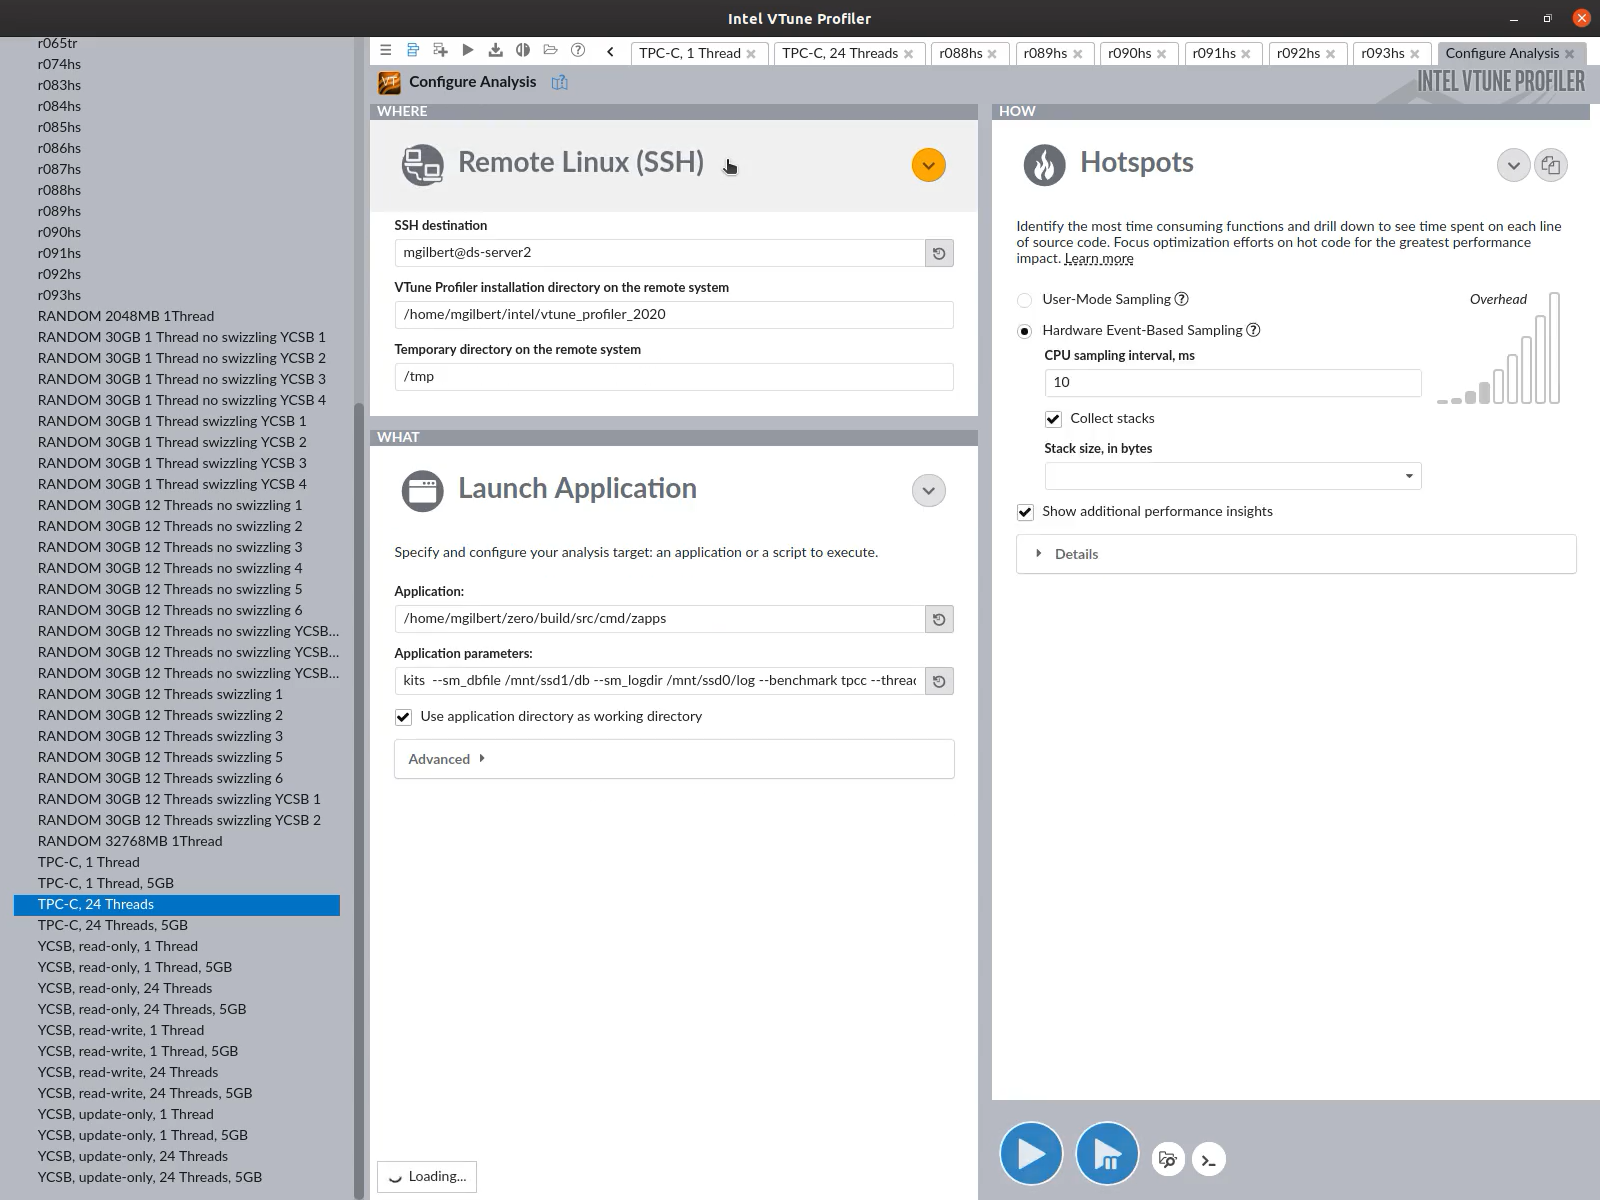
\includegraphics[width = .9\paperheight]{data/where.png}}{data/where.mov}
\end{frame}

\begin{frame}
    \frametitle{Analysis Configuration: What?}
    
    \centering    
    \movie[label = what,
    width = .9\paperheight,
    poster,
    autostart,
    showcontrols,
    loop]{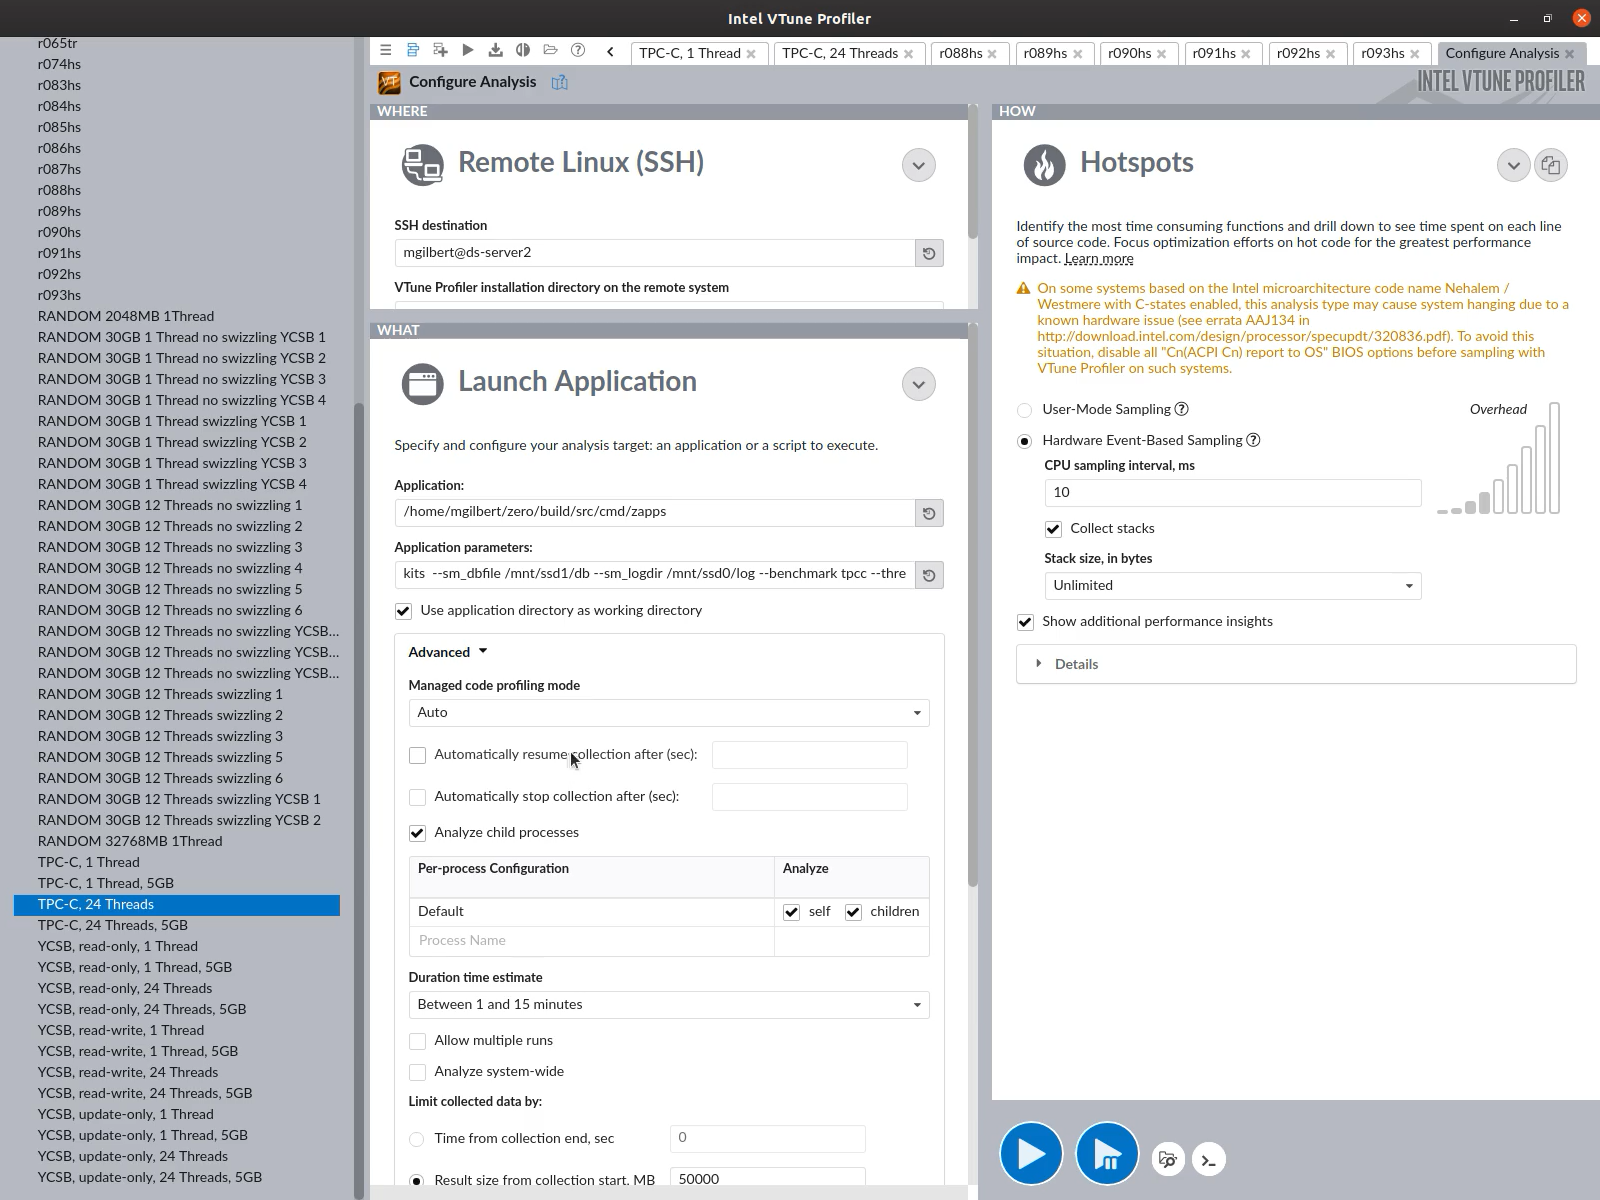
\includegraphics[width = .9\paperheight]{data/what.png}}{data/what.mov}
\end{frame}

\begin{frame}
    \frametitle{Analysis Configuration: How?}
    
    \centering    
    \movie[label = how,
    width = .9\paperheight,
    poster,
    autostart,
    showcontrols,
    loop]{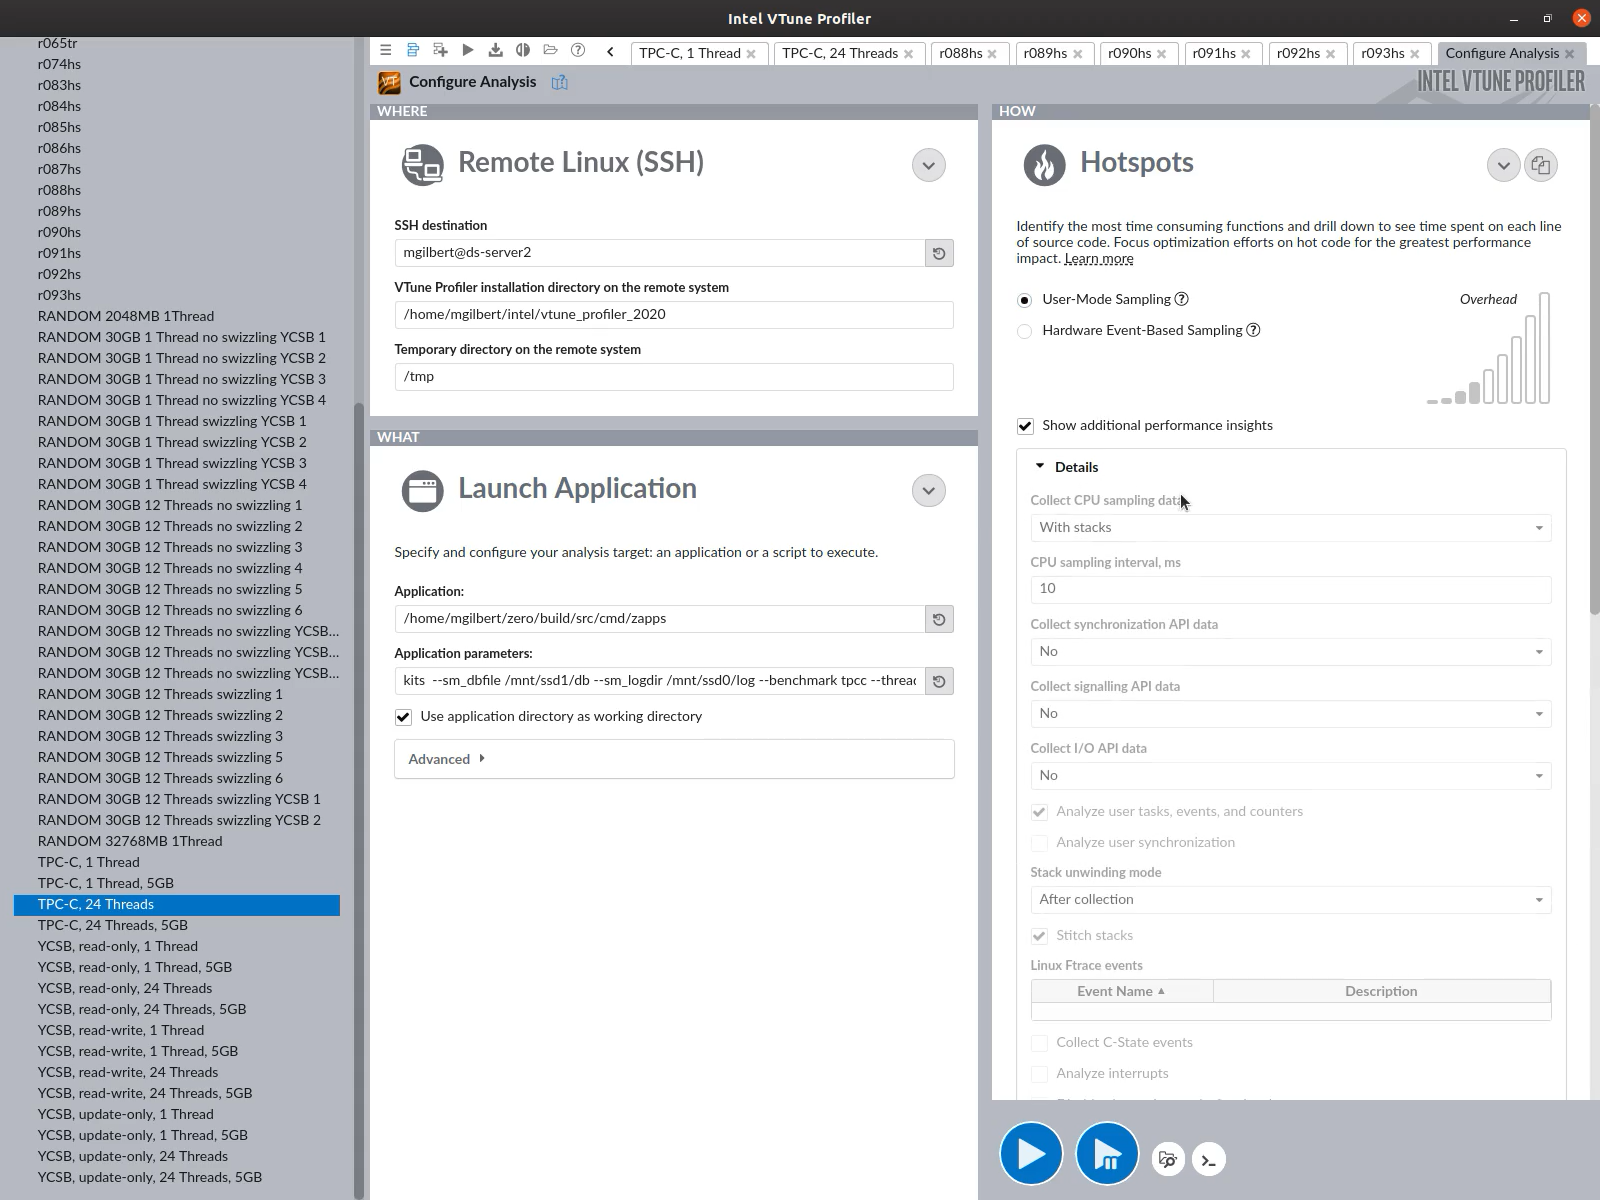
\includegraphics[width = .9\paperheight]{data/how.png}}{data/how.mov}
\end{frame}

\begin{frame}
    \frametitle{Analysis Configuration: How??}
    
    \centering    
    \movie[label = how2,
    width = .9\paperheight,
    poster,
    autostart,
    showcontrols,
    loop]{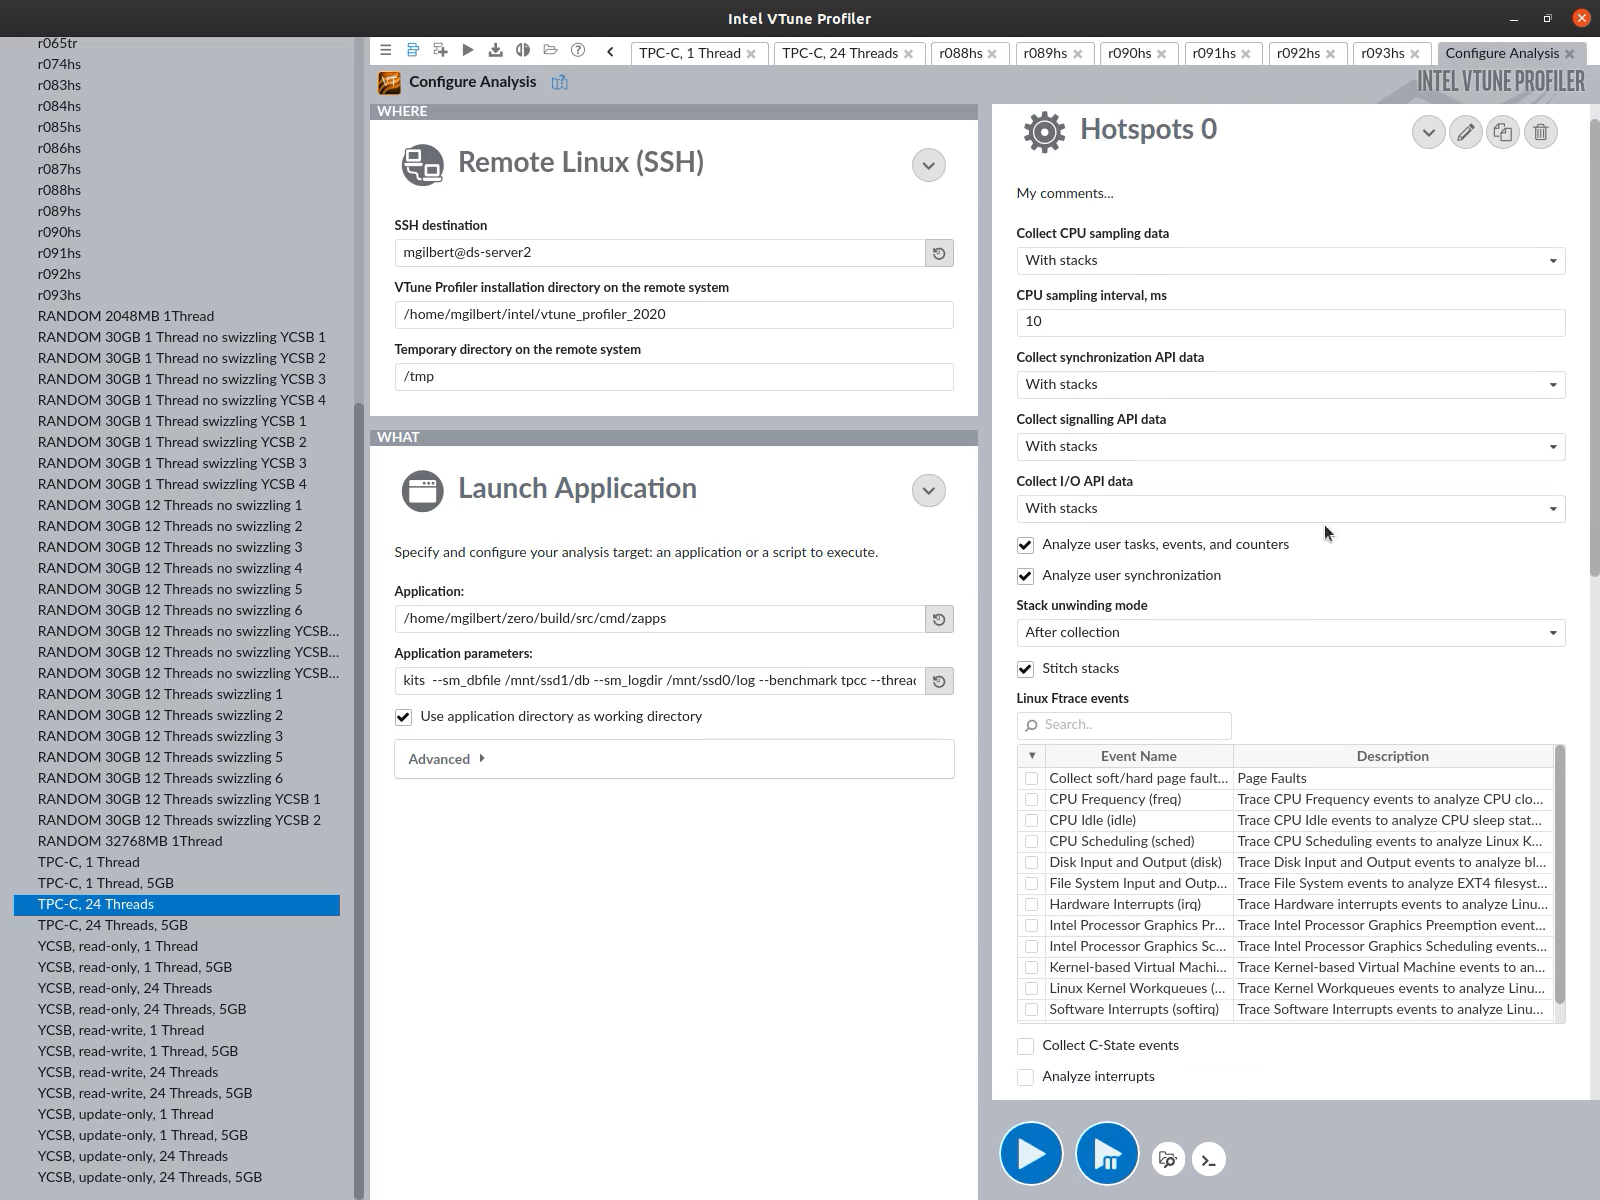
\includegraphics[width = .9\paperheight]{data/how_details.png}}{data/how_details.mov}
\end{frame}

\begin{frame}
    \frametitle{Analysis: Open}
    
    \centering    
    \movie[label = open,
    width = .9\paperheight,
    poster,
    autostart,
    showcontrols,
    loop]{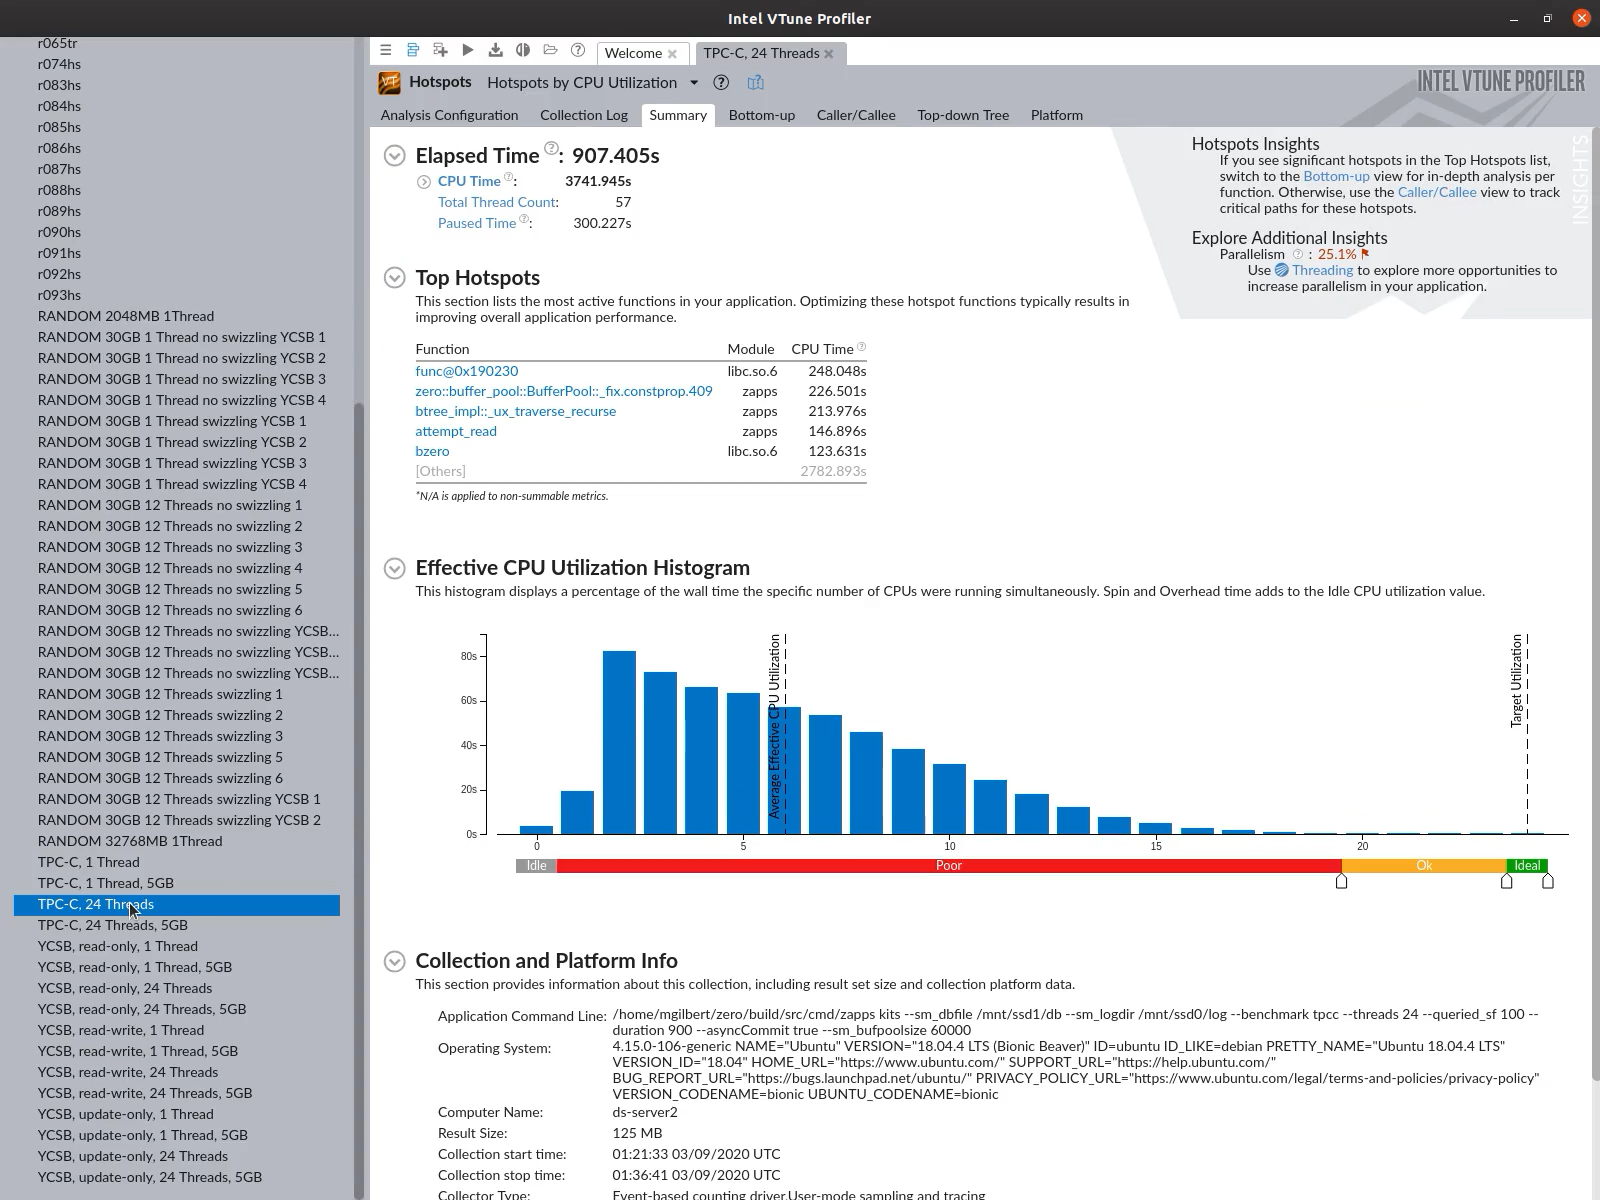
\includegraphics[width = .9\paperheight]{data/open_analysis.png}}{data/open_analysis.mov}
\end{frame}

\begin{frame}
    \frametitle{Analysis: Configuration \& Collection Log}
    
    \centering    
    \movie[label = log,
    width = .9\paperheight,
    poster,
    autostart,
    showcontrols,
    loop]{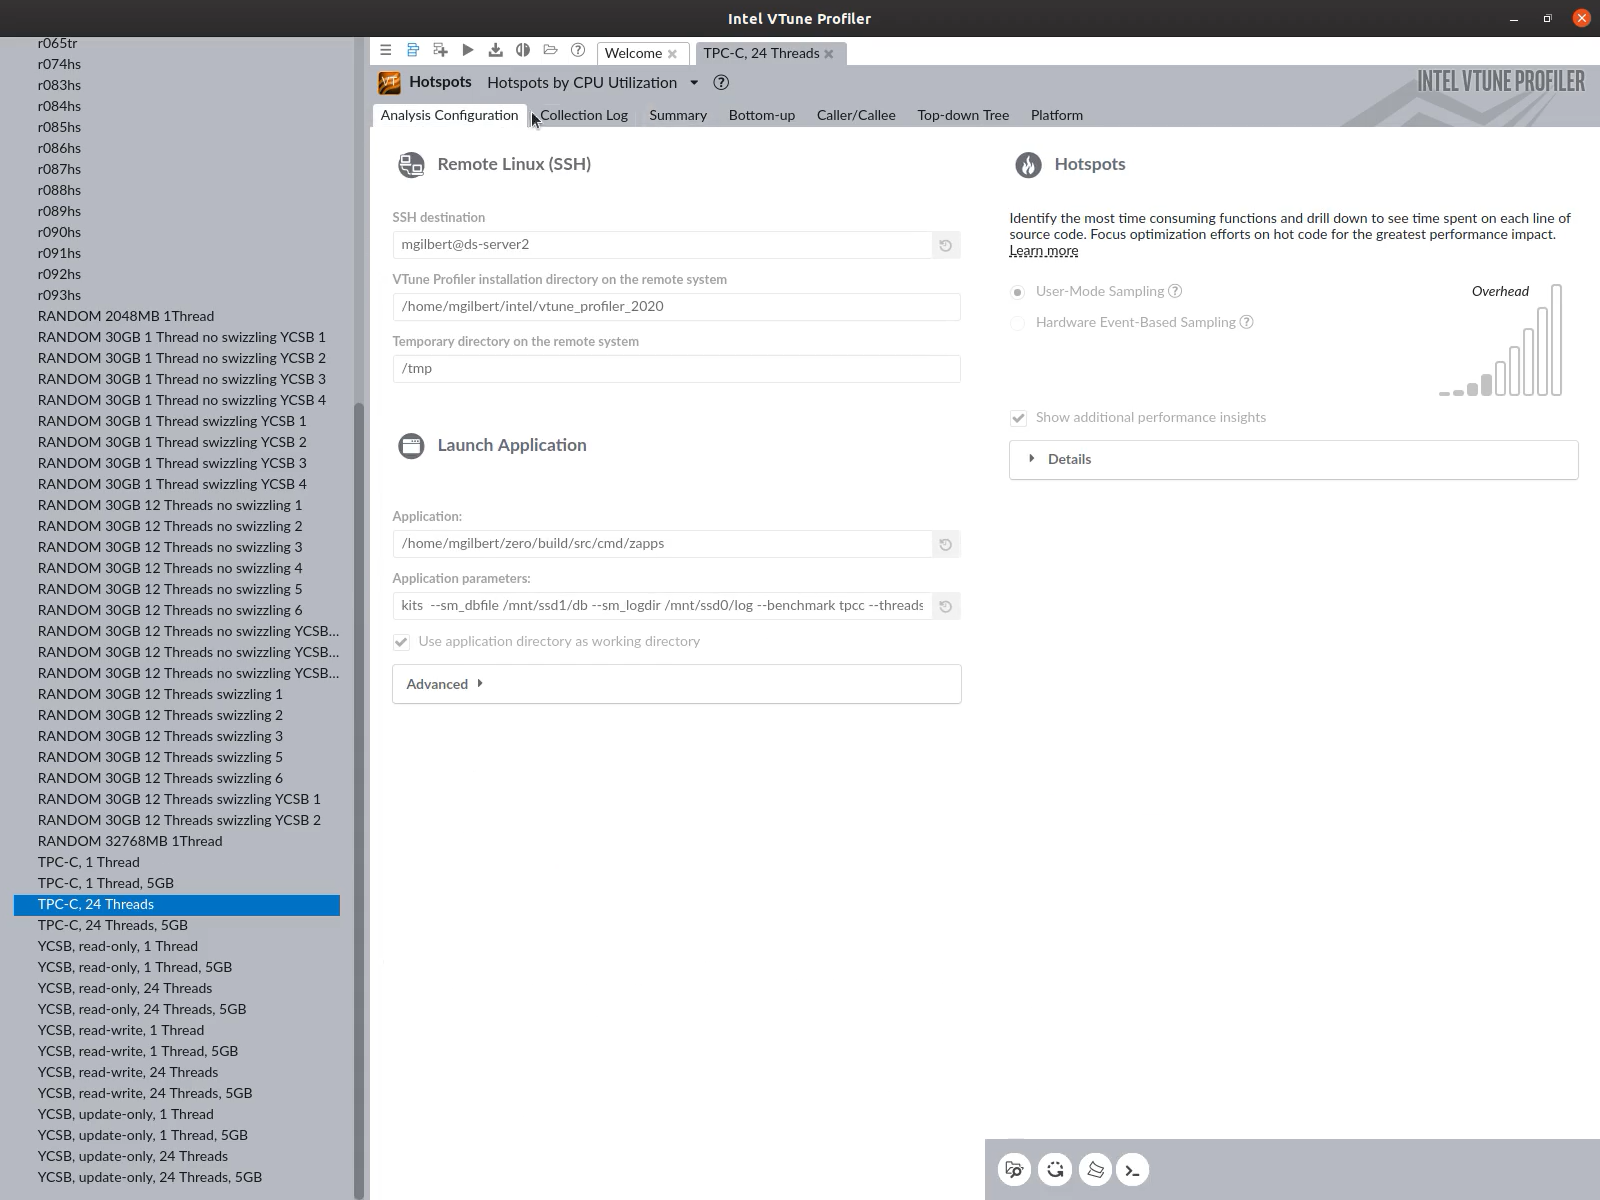
\includegraphics[width = .9\paperheight]{data/analysis_configuration_collection_log.png}}{data/analysis_configuration_collection_log.mov}
\end{frame}

\begin{frame}
    \frametitle{Analysis: Summary}
    
    \centering    
    \movie[label = summary,
    width = .9\paperheight,
    poster,
    autostart,
    showcontrols,
    loop]{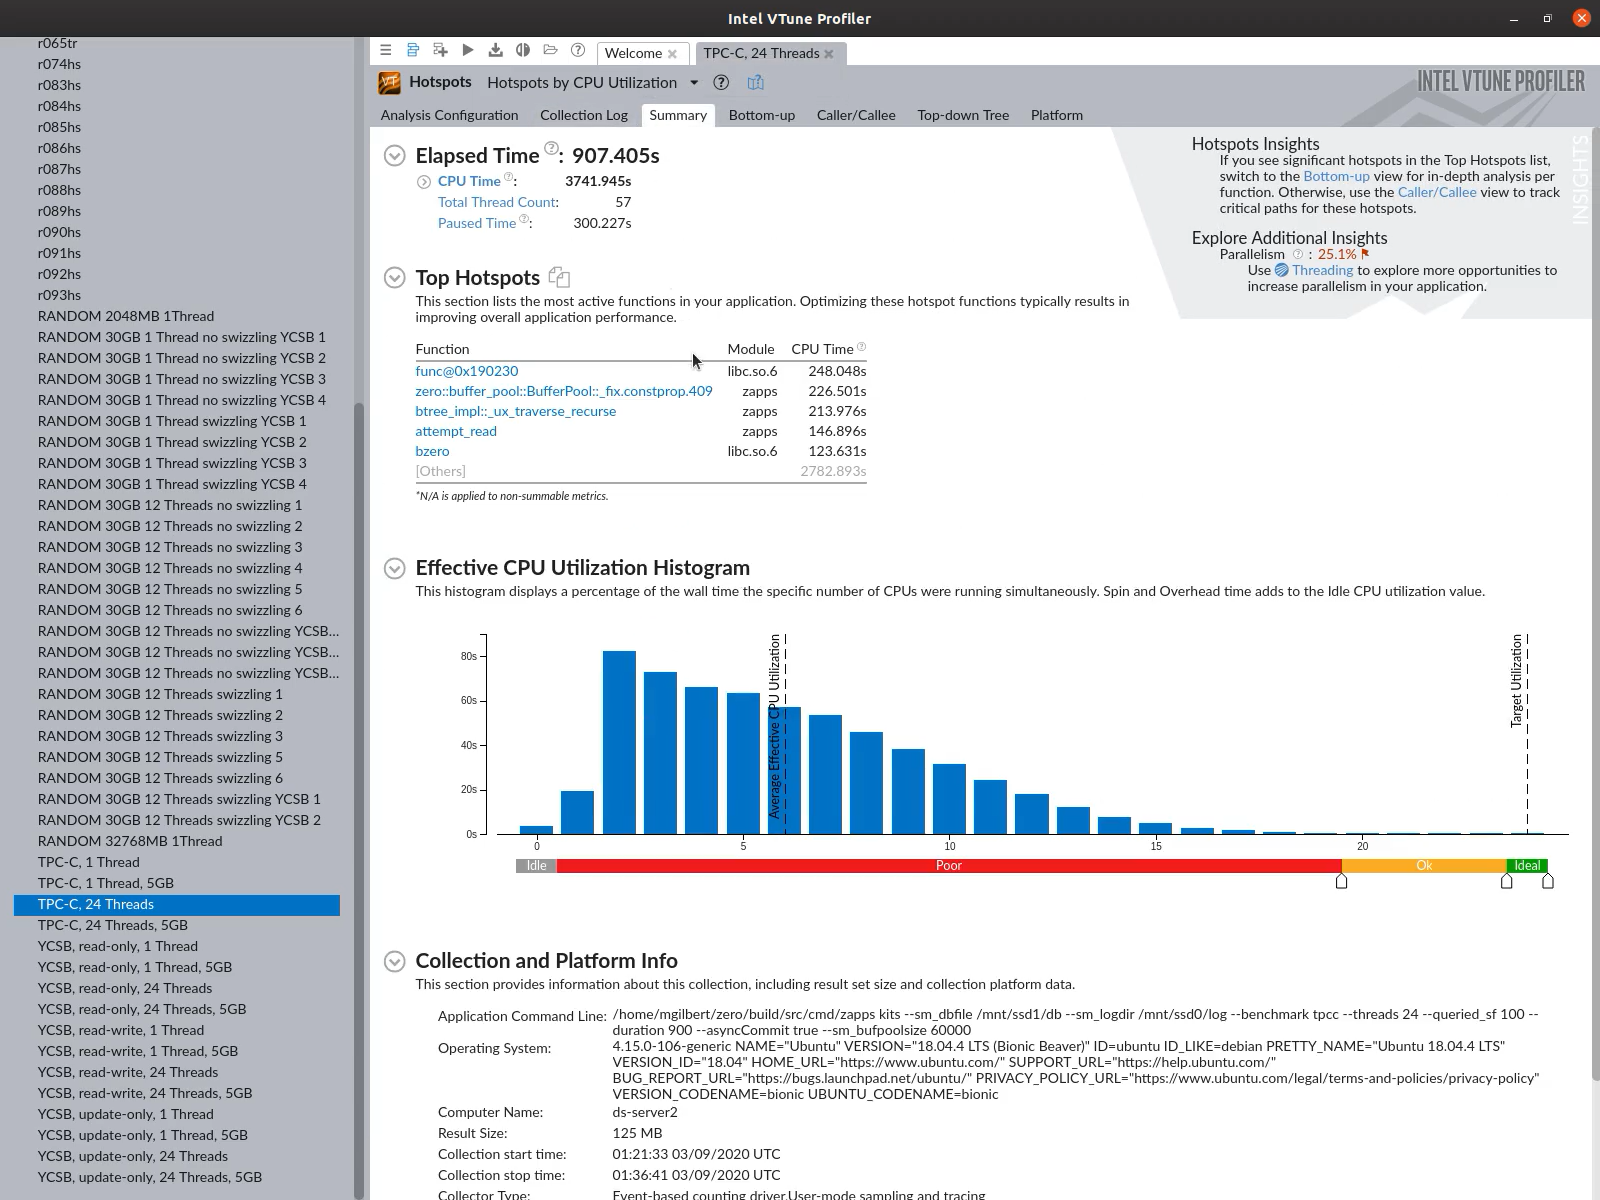
\includegraphics[width = .9\paperheight]{data/summary.png}}{data/summary.mov}
\end{frame}

\begin{frame}
    \frametitle{Analysis: Bottom-Up}
    
    \centering    
    \movie[label = bottom-up,
    width = .9\paperheight,
    poster,
    autostart,
    showcontrols,
    loop]{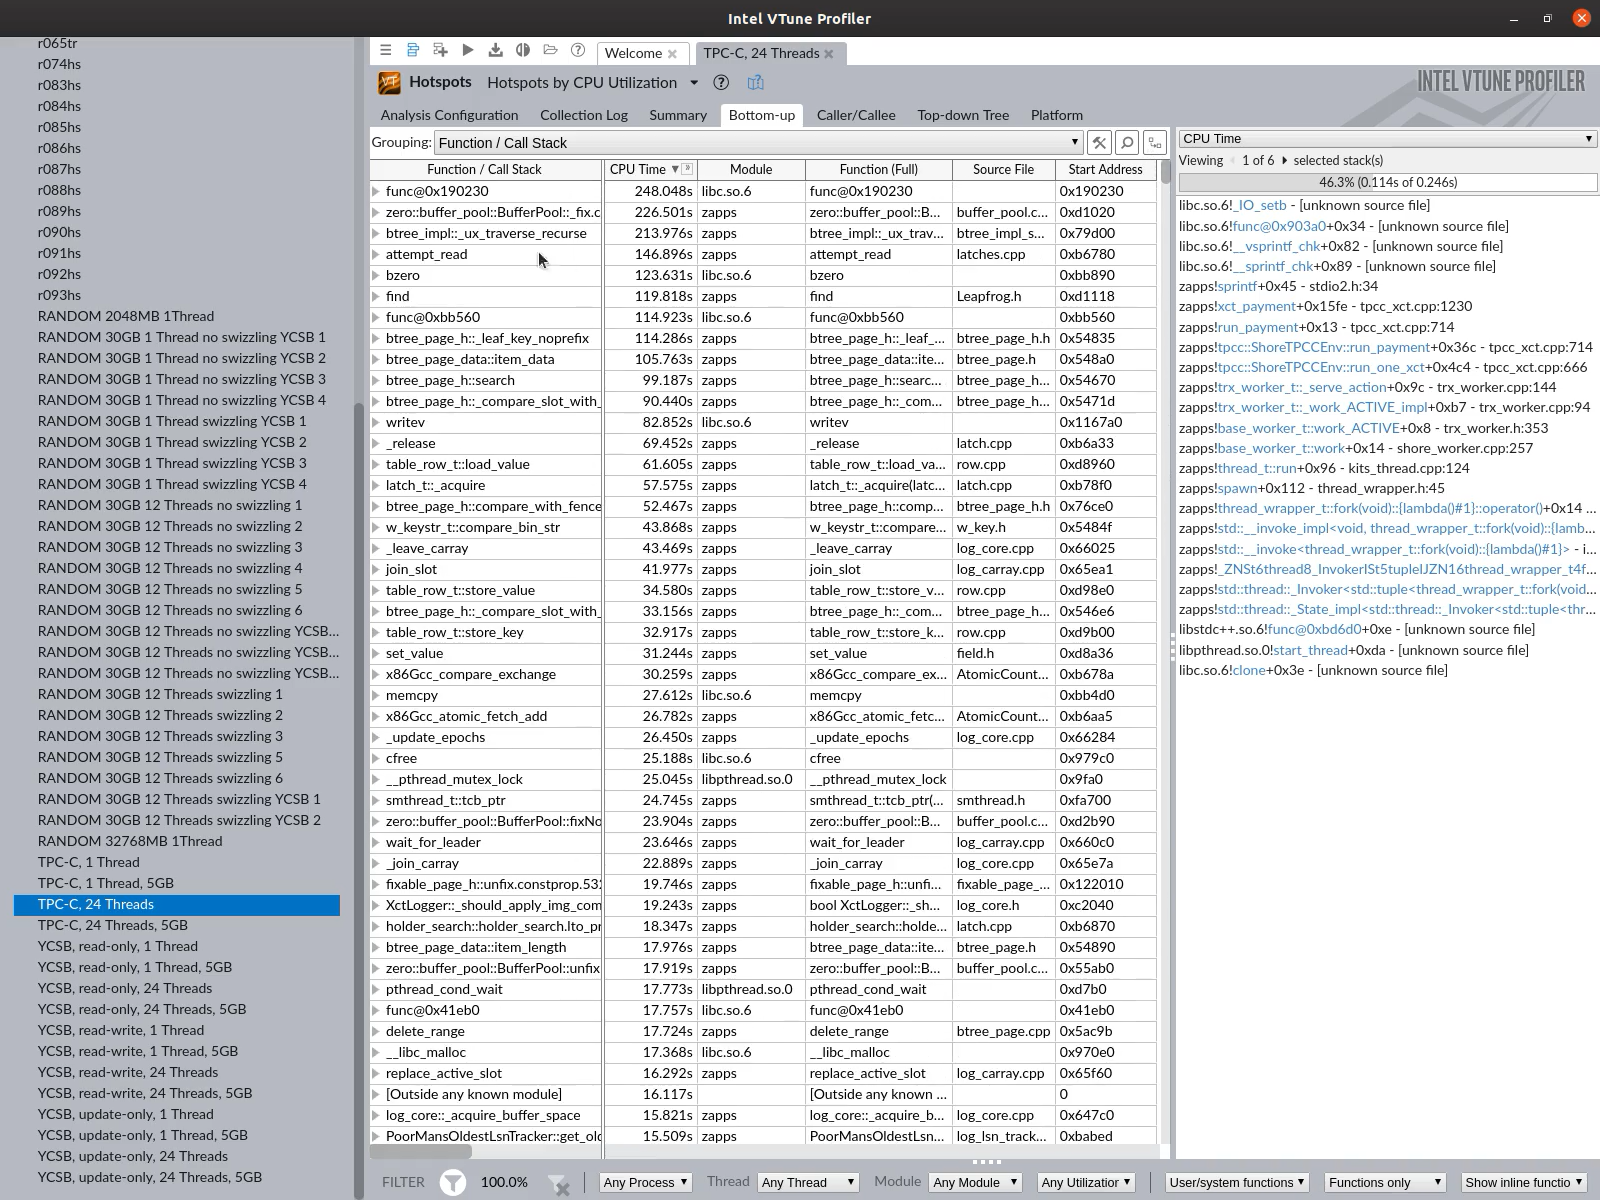
\includegraphics[width = .9\paperheight]{data/bottom-up.png}}{data/bottom-up.mov}
\end{frame}

\begin{frame}
    \frametitle{Analysis: Caller/Callee}
    
    \centering    
    \movie[label = caller_callee,
    width = .9\paperheight,
    poster,
    autostart,
    showcontrols,
    loop]{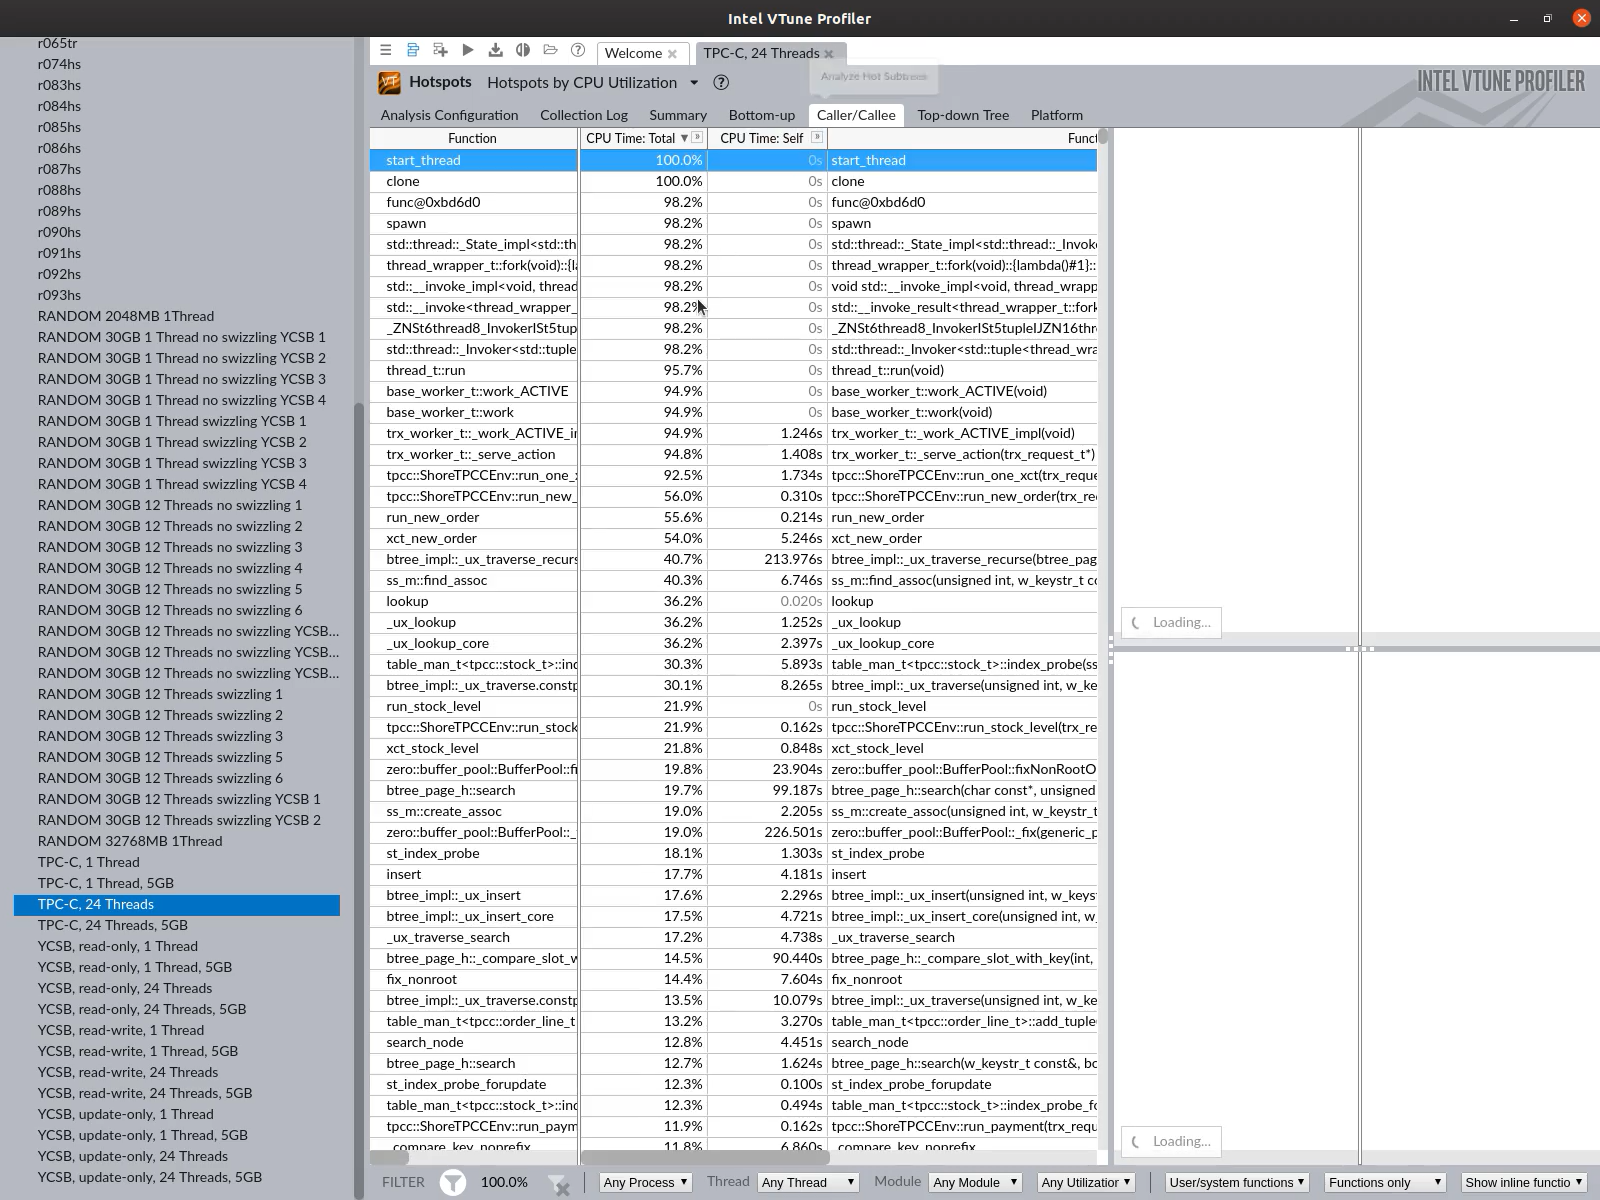
\includegraphics[width = .9\paperheight]{data/caller_callee.png}}{data/caller_callee.mov}
\end{frame}

\begin{frame}
    \frametitle{Analysis: Top-Down Tree}
    
    \centering    
    \movie[label = topdowntree,
    width = .9\paperheight,
    poster,
    autostart,
    showcontrols,
    loop]{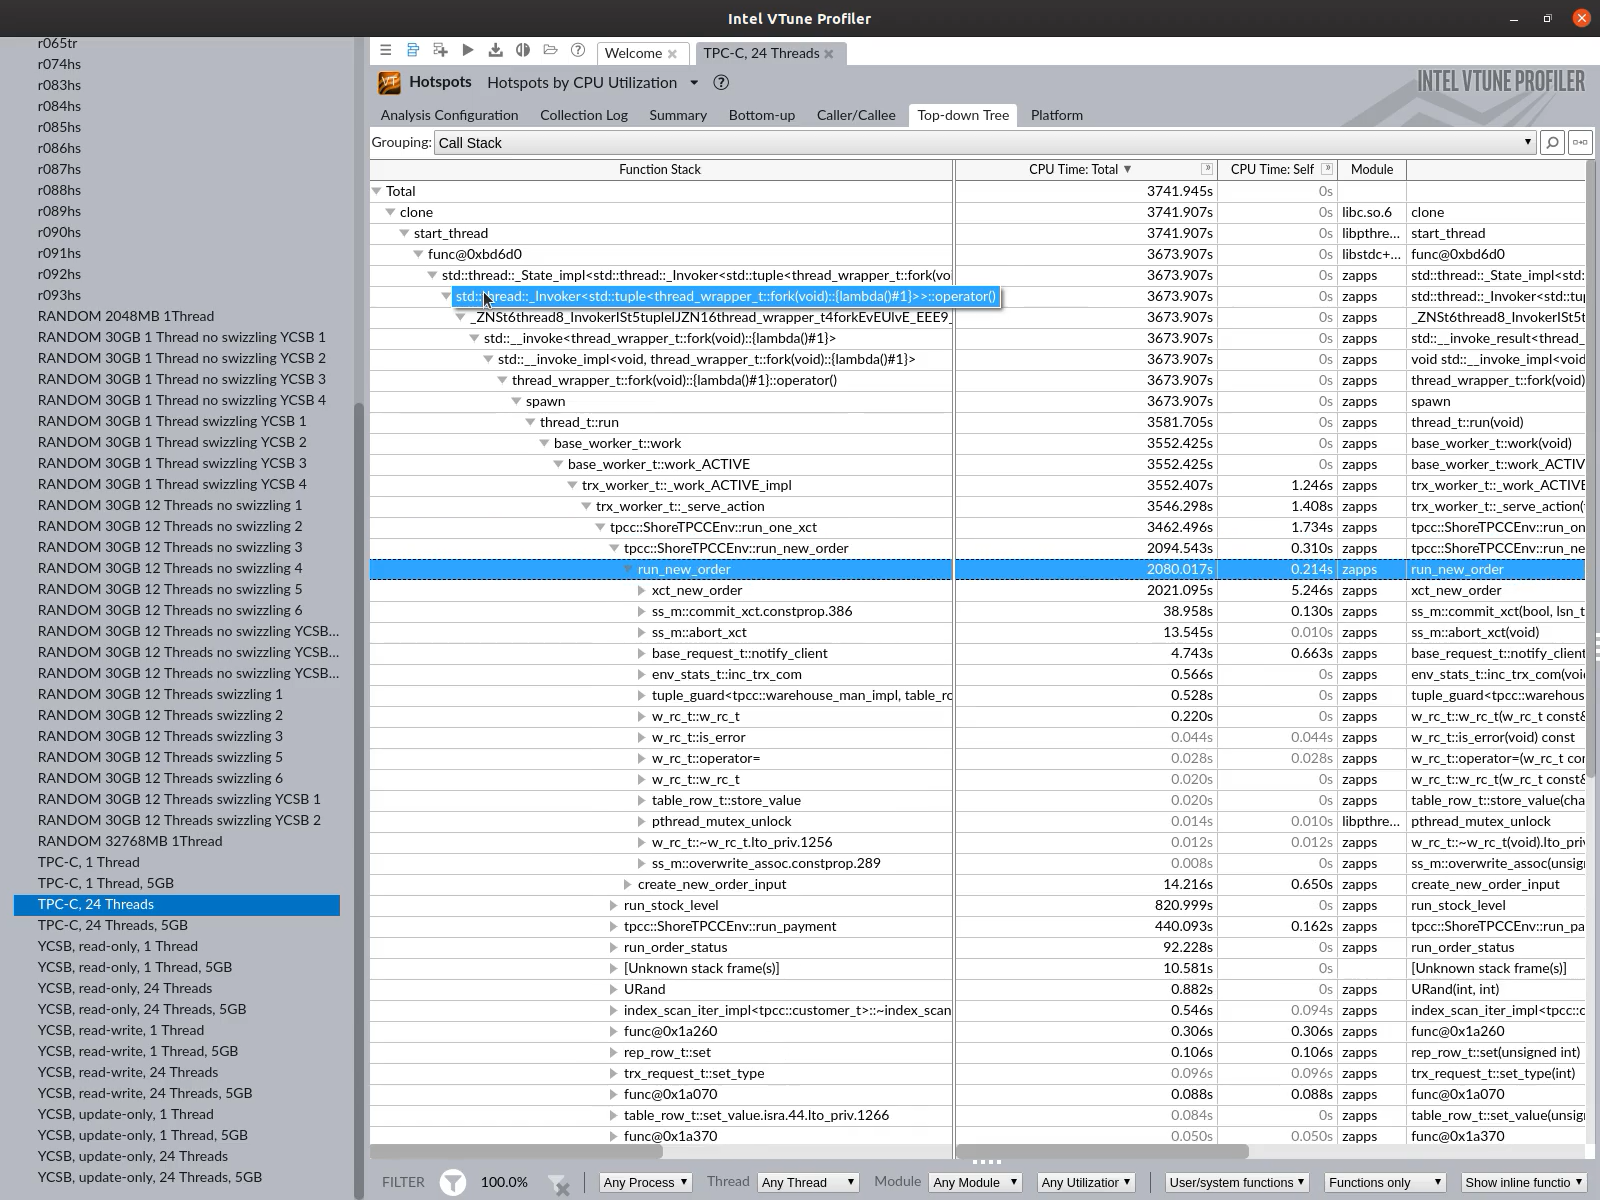
\includegraphics[width = .9\paperheight]{data/top-down_tree.png}}{data/top-down_tree.mov}
\end{frame}

\begin{frame}
    \frametitle{Analysis: Filter}
    
    \centering    
    \movie[label = filter,
    width = .9\paperheight,
    poster,
    autostart,
    showcontrols,
    loop]{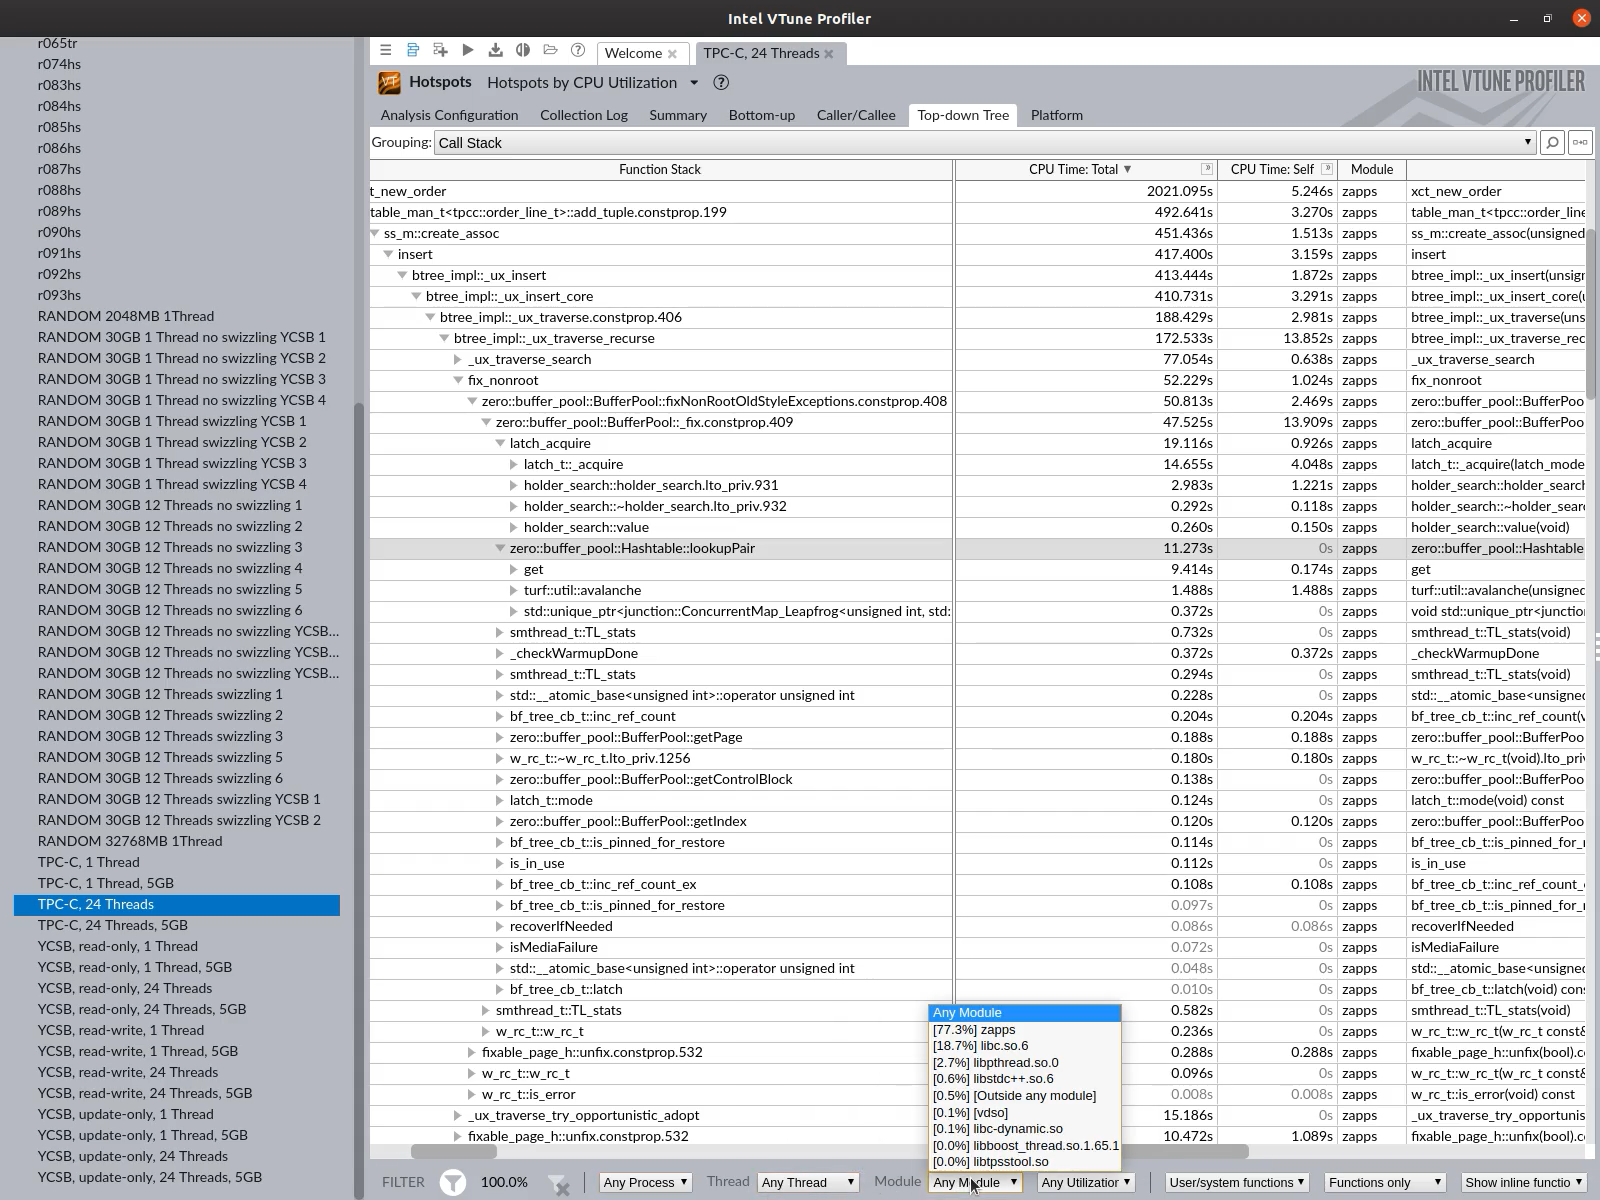
\includegraphics[width = .9\paperheight]{data/filter.png}}{data/filter.mov}
\end{frame}

\begin{frame}
    \frametitle{Analysis: Filter in Time}
    
    \centering    
    \movie[label = timefilter,
    width = .9\paperheight,
    poster,
    autostart,
    showcontrols,
    loop]{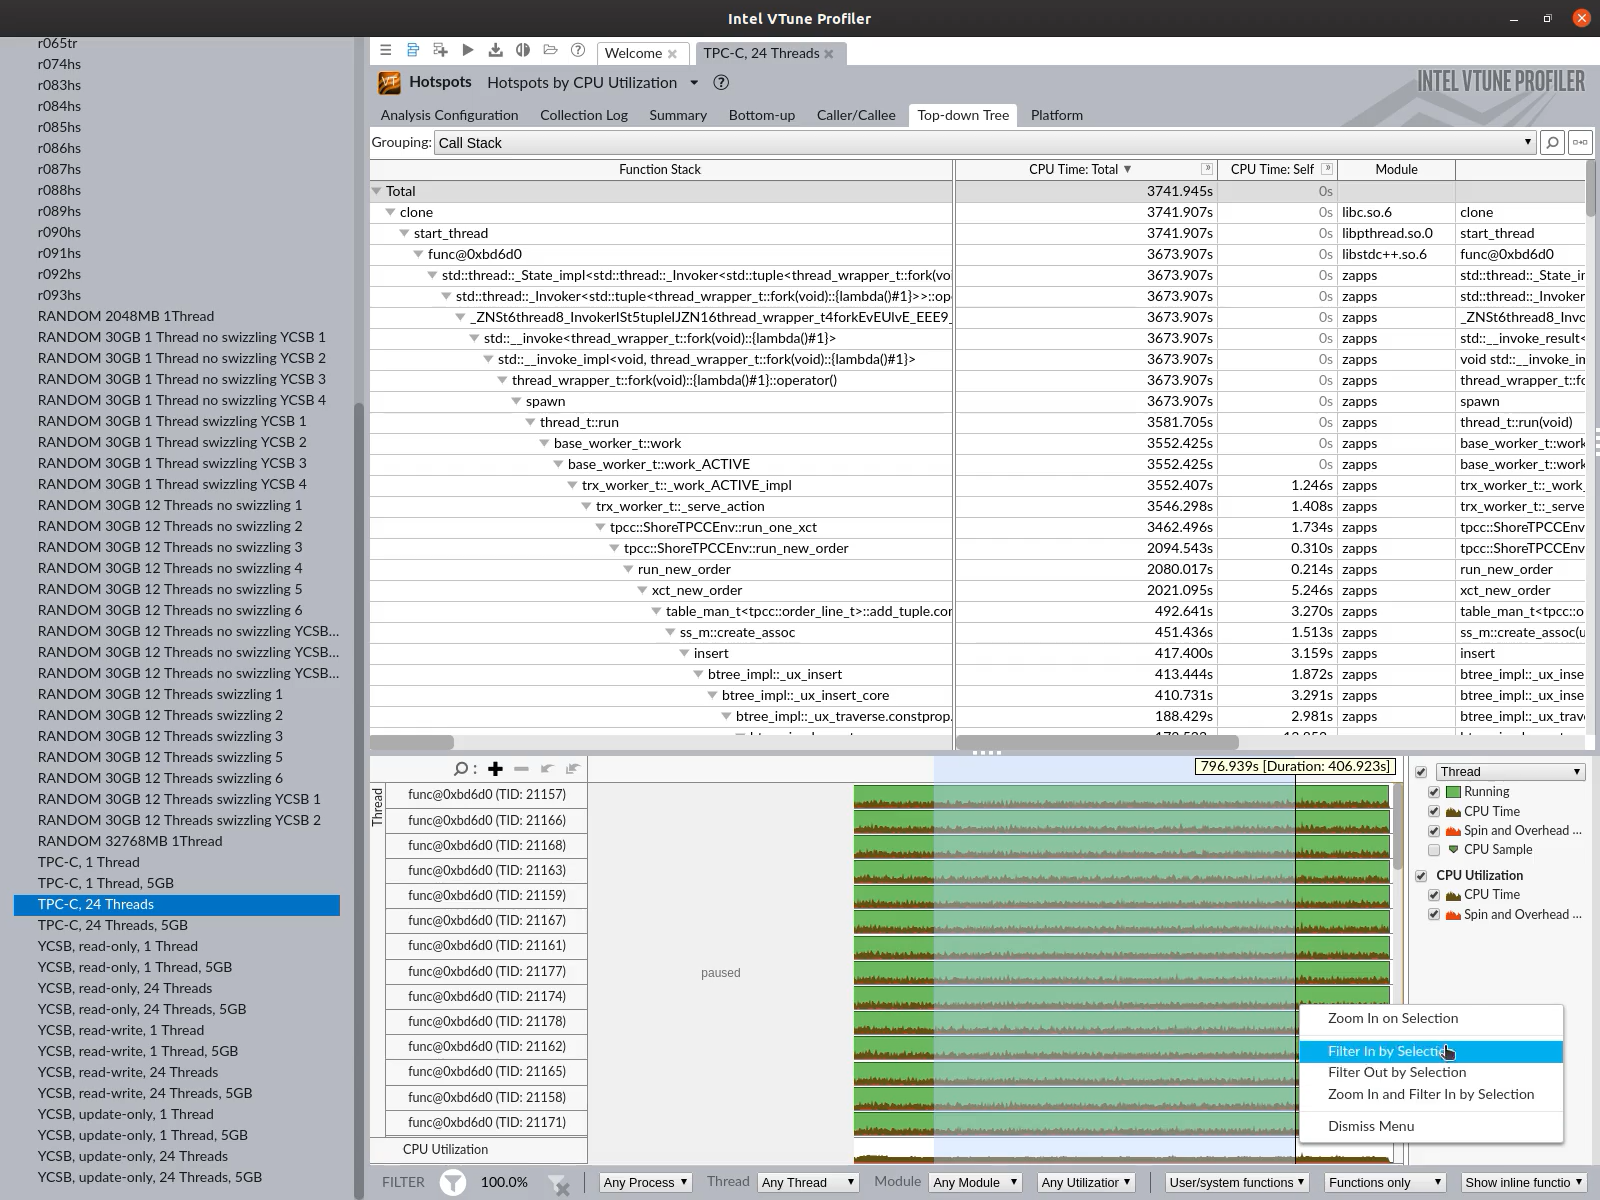
\includegraphics[width = .9\paperheight]{data/filter_time.png}}{data/filter_time.mov}
\end{frame}

\begin{frame}
    \frametitle{Analysis: Platform}
    
    \centering    
    \movie[label = platform,
    width = .9\paperheight,
    poster,
    autostart,
    showcontrols,
    loop]{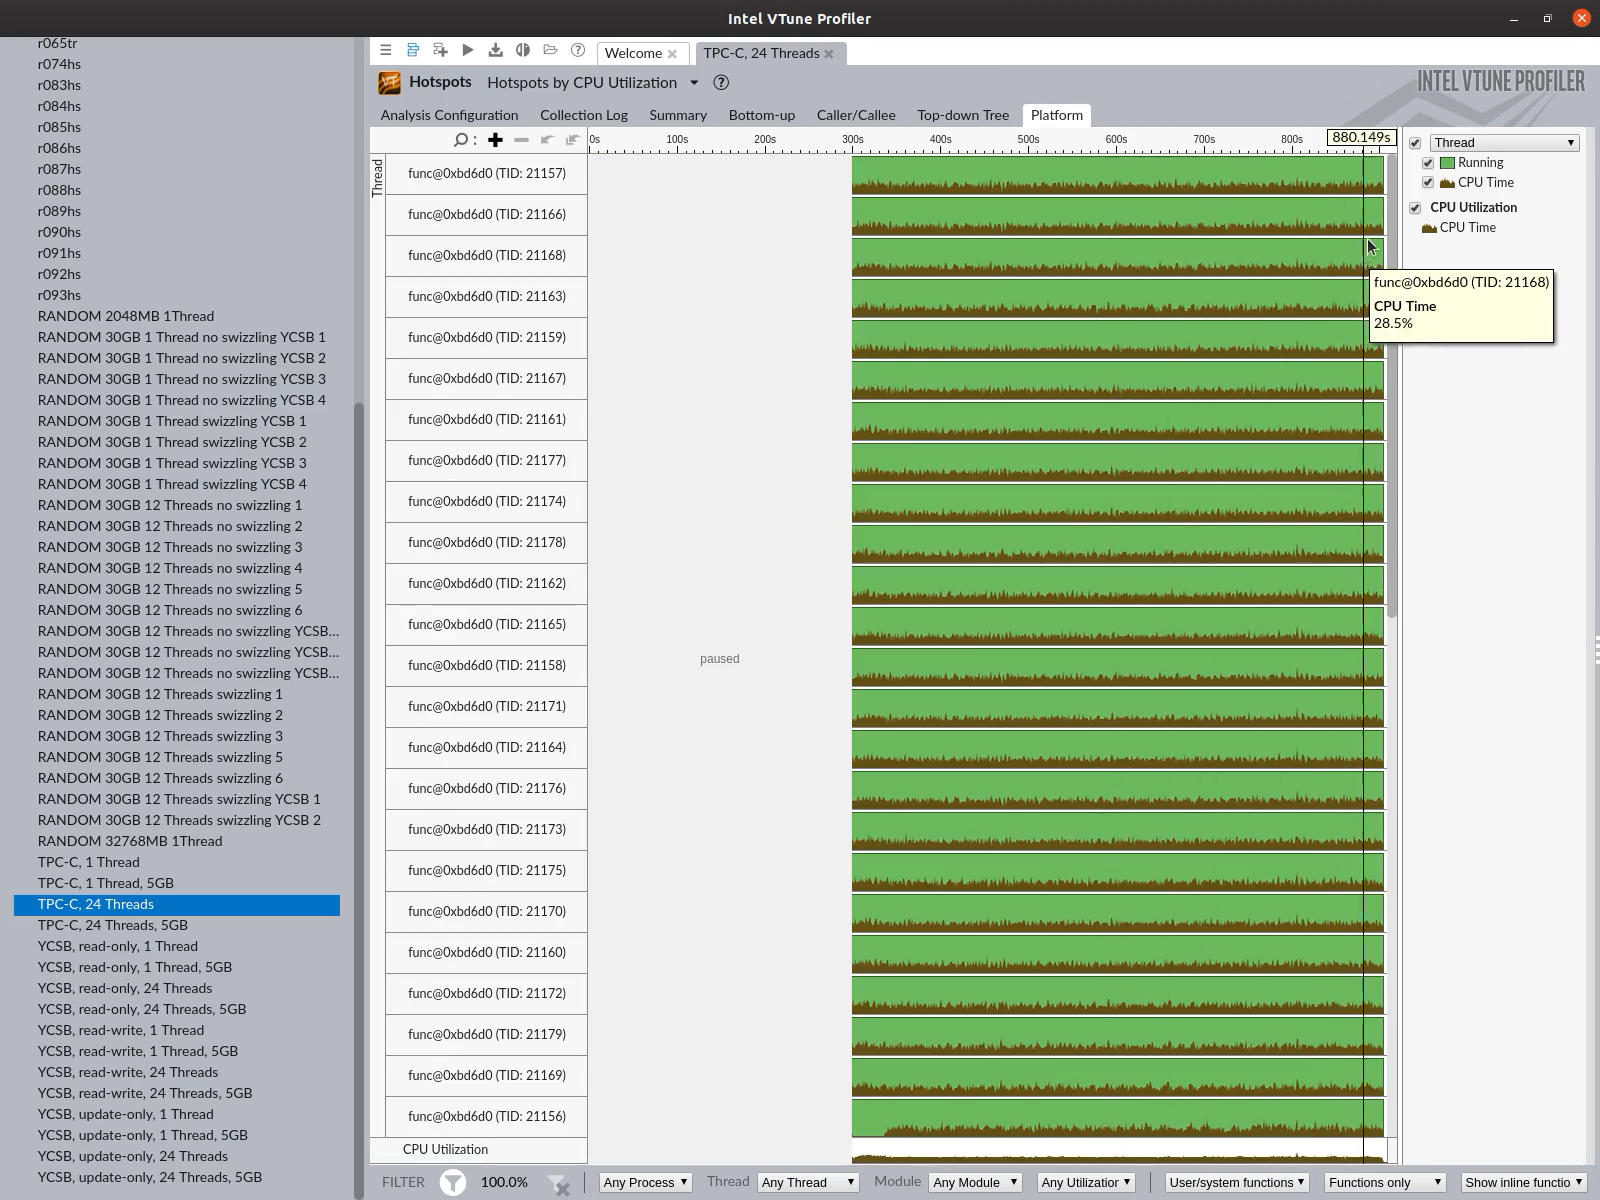
\includegraphics[width = .9\paperheight]{data/platform.png}}{data/platform.mov}
\end{frame}


%----------------------------------------------------------------------------------------

\end{document} 